\documentclass[12pt,a4paper]{book}

\usepackage [utf8] {inputenc}
\usepackage [russian] {babel}
\usepackage {graphicx}
\usepackage {amsmath}
\usepackage {color}
\usepackage [hidelinks]{hyperref}
\usepackage {floatflt}
\usepackage [nounderscore]{syntax}

\usepackage {styles/text}
\usepackage {styles/listings}

\graphicspath{{img/}}

\hypersetup{
	colorlinks=true,
	linkcolor=blue,          % color of internal links
	citecolor=blue,        % color of links to bibliography
	filecolor=blue,      % color of file links
	urlcolor=blue           % color of external links
}

\begin {document}

\title{Разработка программ с помощью Objective Caml\\
Developing Applications with Objective Caml}
\author{Emmanuel Chailloux\\ Pascal Manoury\\ Bruno Pagano}

\maketitle

 

 


\tableofcontents

\chapter{Как заполучить Objective CAML}


\part{Основы языка}
\chapter{Функциональное программирование}

\section{Введение}
\label{sec:intro_2}

Первый язык функционального программирования LISP появился в конце 1950, в тот
же момент, что и Fortran --- один из первых императивных языков. Оба этих языка
существуют и по сей день, хотя они немало изменились. Область их применения:
вычислительные задачи для Фортрана и символьные (symbolic) для Lisp. Интерес к
функциональному программированию состоит в простоте написания программ, где под
программой подразумевается функция, применённая к аргументам. Она вычисляет
результат, который возвращается как вывод программы. Таким образом можно с
лёгкостью комбинировать программы: вывод одной, становится входным аргументом
для другой.

Функциональное программирование основывается на простой модели вычислений,
состоящей из трёх конструкций: переменные, определение функции и её применение к
какому--либо аргументу. Эта модель, называемая $\lambda$--исчисление, была
введена Alonzo Church в 1932, ещё до появления первых компьютеров. В
$\lambda$--исчислении любая функция является переменной, так что она может быть
использована как входной параметр другой функции, или возвращена как результат
другой. Теория $\lambda$--исчисления утверждает что все то, что вычисляемо может
быть представлено этим формализмом. Однако, синтаксис этой теории слишком
ограничен, чтобы его можно было использовать его как язык программирования. В
связи с этим к $\lambda$--исчислению были добавлены базовые типы (например,
целые числа или строки символов), операторы для этих типов, управляющие
структуры и объявление позволяющие именовать переменные или функции, и в
частности рекурсивные функции.

Существует разные классификации языков функционального программирования. Мы
будем различать их по двум характеристикам, которые нам кажутся наиболее
важными:

\begin{itemize}
	\item без побочных эффектов (чистые), или с побочным эффектом
(не чистые): чистый язык --- это тот, в котором не существует изменения
состояния. Все есть вычисление, и как оно происходит, нас не интересует. Не
чистые языки, такие как Caml или ML, имеют императивные особенности, такие как
изменение состояния. Они позволяют писать программы в стиле близкому к Фортрану,
в котором важен порядок вычисления выражений.

	\item язык типизирован динамически или статически: типизация необходима для
проверки соответствия аргумента, переданного функции, типу формального
параметра. Это проверка может быть выполнена во время выполнения программы. В
этом случае типизация называется динамической. В случае ошибки программа будет
остановлена, как это происходит в Lisp. В случае статической типизации проверка
осуществляется во время компиляции, то есть до выполнения программы. Таким
образом она (проверка) не замедлит программу во время выполнения. Эта типизация
используется в ML и в его диалектах, таких как Objective CAML. Только правильно
типизированные программы, то есть успешно прошедшие проверку типов, могут быть
скомпилированы и затем выполнены.
\end{itemize}

\section{План главы}
\label{sec:chapter_outline_2}

В этой главе представлены базовые элементы функциональной части языка Objective
CAML, а именно: синтаксис, типы и механизм исключений. После этого вводного
курса мы сможем написать нашу первую программу.

В первом разделе описаны основы языка, начиная с базовых типов и функций. Затем
мы рассмотрим структурные и функциональные типы. После этого мы рассмотрим
управляющие структуры, а также локальные и глобальные объявления. Во втором
разделе мы обсудим определение типов для создания структур и механизм
сопоставления с образцом, который используется для доступа к этим структурам. В
третьем разделе рассматривается выводимый тип функций и область их применения,
после чего следует описание механизма исключений. Четвёртый раздел объединяет
введённые понятия в простой пример программы--калькулятора.

\section{Функциональное ядро Objective CAML}
\label{sec:caml_kernel}

Как любой другой язык функционального программирования, Objective CAML --- это
язык выражений, состоящий в основном из создания функций и их применения.
Результатом вычисления одного из таких выражений является значение данного языка
(value in the language) и выполнение программы заключается в вычислении всех
выражений из которых она состоит.

\subsection{Значения, функции и базовые типы}
\label{sec:values_funcs_base_types}

В Objective CAML определены следующие типы: целые числа, числа с плавающей
запятой, символьный, строковый и логический.

\subsubsection{Числа}

Различают целые \texttt{int} и числа с плавающей запятой \texttt{float}.
Objective CAML следует спецификации IEEE 754 для представления чисел с плавающей
запятой двойной точности. Операции с этими числами описаны в таблице
\ref{tbl:operations_on_numbers}. Если результат целочисленной операции выходит
за интервал значений типа \texttt{int}, то это не приведёт к ошибке. Результат
будет находиться в интервале целых чисел, то есть все действия над целыми
ограниченны операцией \texttt{modulo} с границами интервала.

\begin{table}[hl]
\begin{center}
	\caption{Операции над числами}
	\begin{tabular}{|p{7.2cm}|p{7.2cm}|}
	\hline
	целые & плавающие \\
	\hline
	+ сложение & +. сложение \\
	\hline
	- вычитание и унарный минус & -. вычитание и унарный минус \\
	\hline
	* умножение & *. умножение \\
	\hline
	/ деление & /. деление \\
	\hline
	\texttt{mod} остаток целочисленного деления & ** возведение в степень \\
	\hline
	\end{tabular}
%\vspace{12}
	\begin{tabular}{|p{7.2cm}|p{7.2cm}|}
	\hline
{\begin{lstlisting}[language=OCaml,frame=none]
# 1 ;;
- : int = 1
# 1 + 2 ;;
- : int = 3
# 9 / 2 ;;
- : int = 4
# 11 mod 3 ;;
- : int = 2
(* limits of the representation  *)
(* of integers                   *)
# 2147483650 ;;
- : int = 2
\end{lstlisting}}
 &
{\begin{lstlisting}[language=OCaml,frame=none]
# 2.0 ;;
- : float = 2
# 1.1 +. 2.2 ;;
- : float = 3.3
# 9.1 /. 2.2 ;;
- : float = 4.13636363636
# 1. /. 0. ;;
- : float = inf
(* limits of the representation  *)
(* of floating-point numbers     *)
# 222222222222.11111 ;;
- : float = 222222222222
\end{lstlisting}}
\\
	\hline
	\end{tabular}
	\label{tbl:operations_on_numbers}
\end{center}
\end{table}

\subsubsection{Разница между целыми числами и числами с плавающей запятой.}

Значения разных типов, таких как \texttt{float} и \texttt{int}, не могут
сравниваться между собой напрямую. Для этого существует функции перевода одного
типа в другой (\texttt{float\_of\_int} и \texttt{int\_of\_float}).

\begin{lstlisting}[language=OCaml]
# 2 = 2.0;;
Error: This expression has type float but an expression was expected of type
         int
# 3.0 = float_of_int 3;;
- : bool = true
\end{lstlisting}

Аналогично, операции над целыми числами и числами с плавающей запятой различны:

\begin{lstlisting}[language=OCaml]
# 3 + 2;;
- : int = 5
# 3.0 +. 2.0;;
- : float = 5.
# 3.0 + 2.0;;
Error: This expression has type float but an expression was expected of type
         int
# sin 3.14159;;
- : float = 2.65358979335273e-06
\end{lstlisting}

Неопределенный результат, например получаемый при делении на ноль, приведет к
возникновению исключения (см. \ref{??}, стр. \pageref{??}), которое остановит
вычисление. Числа с плавающей запятой имеют специальные значения для бесконечных
величин (\texttt{Inf}) и для не определённого результата (\texttt{NaN}
\footnote{Not a Number}). Основные операции над этими числами приведены в
таблице \ref{tbl:functions_on_floats}

\begin{table}[hl]
\begin{center}
	\caption{Функции над числами с плавающей запятой}
	\begin{tabular}{|p{7.2cm}|p{7.2cm}|}
	\hline
	\texttt{ceil} & \texttt{cos} косинус \\
	\hline
	\texttt{floor} & \texttt{sin} синус \\
	\hline
	\texttt{sqrt} --- квадратный корень & \texttt{tan} тангенс \\
	\hline
	\texttt{exp} --- экспонента & \texttt{acos} арккосинус \\
	\hline
	\texttt{log} --- натуральный логарифм & \texttt{asin} арксинус \\
	\hline
	\texttt{log10} --- логарифм по базе 10 & \texttt{atan} арктангенс \\
	\hline
	\end{tabular}
%\vspace{12}
	\begin{tabular}{|p{7.2cm}|p{7.2cm}|}
	\hline
{\begin{lstlisting}[language=OCaml,frame=none]
# ceil 3.4 ;;
- : float = 4.
# floor 3.4 ;;
- : float = 3.
# ceil (-.3.4) ;;
- : float = -3.
# floor (-.3.4) ;;
- : float = -4.
\end{lstlisting}}
 &
{\begin{lstlisting}[language=OCaml,frame=none]
# sin 1.57078 ;;
- : float = 0.999999999866717837
# sin (asin 0.707) ;;
- : float = 0.707
# acos 0.0 ;;
- : float = 1.57079632679489656
# asin 3.14 ;;
- : float = nan
\end{lstlisting}}
\\
	\hline
	\end{tabular}
	\label{tbl:functions_on_floats}
\end{center}
\end{table}

\subsubsection{Символы и строки}

Символы, тип \texttt{char}, соответствуют целым числам в интервале от 0 до 255,
первые 128 значений соответствуют кодам ASCII. Функция \texttt{char\_of\_int} и
\texttt{int\_of\_char} преобразуют один тип в другой. Строки, тип
\texttt{string} --- это последовательность символов определенной длинны (не
длиннее $224^{24} - 6$). Оператором объединения строк (конкатенации) является
шапка $\wedge$. Следующие функции необходимы для перевода типов
\texttt{int\_of\_string}, \texttt{string\_of\_int}, \texttt{string\_of\_float} и
\texttt{float\_of\_string}.

\begin{lstlisting}[language=OCaml]
# 'B' ;;
- : char = 'B'
# int_of_char 'B' ;;
- : int = 66
# "est une chaîne" ;;
- : string = "est une cha\195\174ne"
# (string_of_int 1987) ^ " est l'année de la création de CAML" ;;
- : string = "1987 est l'ann\195\169e de la cr\195\169ation de CAML"
\end{lstlisting}

Если строка состоит из цифр, то мы не сможем использовать ее в численных
операциях, не выполнив явного преобразования.

\begin{lstlisting}[language=OCaml]
# "1999" + 1 ;;
Error: This expression has type string but an expression was expected of type
         int
# (int_of_string "1999") + 1 ;;
- : int = 2000
\end{lstlisting}

В модуле \texttt{String} собрано много функций для работы со строками (стр.
\pageref{??})

\subsubsection{Булевый тип}

Значение типа \texttt{boolean} принадлежит множеству состоящему из двух
элементов: \texttt{true} и \texttt{false}. Основные операторы описаны в таблице
\ref{tbl:boolean_operations}. По историческим причинам операторы \texttt{and} и
\texttt{or} имеют две формы.

\begin{table}[hl]
\begin{center}
	\caption{Булевы операторы}
	\begin{tabular}{|p{5cm}|p{5cm}|}
	\hline
	not --- отрицание & \\
	\hline
	\&\& логическое и & \& синоним \&\& \\
	\hline
	|| логическое или & \texttt{or} синоним | \\
	\hline
	\end{tabular}
\end{center}
	\label{tbl:boolean_operations}
\end{table}

\begin{lstlisting}[language=OCaml]
# true ;;
- : bool = true
# not true ;;
- : bool = false
# true && false ;;
- : bool = false
\end{lstlisting}

Операторы \&\& и || или их синонимы, вычисляют аргумент слева и в зависимости от
его значения, вычисляют правый аргумент. Они могут быть переписаны в виде
условной структуры (см. \ref{??} стр. \pageref{??}).

\begin{table}[hl]
\begin{center}
	\caption{Операторы сравнения и равенства}
	\begin{tabular}{|p{5cm}|p{5cm}|}
	\hline
	= равенство структурное & < меньше \\
	\hline
	== равенство физическое & > больше \\
	\hline
	<> отрицание = & <= меньше или равно \\
	\hline
	!= отрицание == & >= больше или равно \\
	\hline
	\end{tabular}
\end{center}
	\label{tbl:comparison_operations}
\end{table}

Операторы сравнения и равенства описаны в таблице
\ref{tbl:comparison_operations}. Это полиморфные операторы, то есть они
применимы как для сравнения двух целых, так и двух строк. Единственное
ограничение это то что операнды должны быть одного типа (см. \ref{} стр.
\pageref{}).

\begin{lstlisting}[language=OCaml]
# 1<=118 && (1=2 || not(1=2)) ;;
- : bool = true
# 1.0 <= 118.0 && (1.0 = 2.0 || not (1.0 = 2.0)) ;;
- : bool = true
# "one" < "two" ;;
- : bool = true
# 0 < '0' ;;
Error: This expression has type char but an expression was expected of type
         int
\end{lstlisting}

Структурное равенство при проверке двух переменных сравнивает значение полей
структуры, тогда как физическое равенство проверяет занимают ли эти переменные
одно и то же место в памяти. Оба оператора возвращают одинаковый результат для
простых типов: \texttt{boolean}, \texttt{char}, \texttt{int} и константные
конструкторы (см. \ref{??} стр. \pageref{??}).

\subsubsection{Осторожно}

Числа с плавающей запятой и строки рассматриваются как структурные типы.

\subsubsection{Объединения}

Тип \texttt{unit} определяет множество из всего одного элемента, обозначается:
()

\begin{lstlisting}[language=OCaml]
# () ;;
- : unit = ()
\end{lstlisting}

Это значение будет широко использоваться в императивных программах (см. \ref{}
стр. \pageref{}), в функциях с побочным эффектом. Функции, результат которых
равен (), соответствуют понятию процедуры, которое отсутствует в Objective CAML,
так же как и аналог типа \texttt{void} в языке C.

\subsubsection{Декартово произведение, кортежи}

Значения разных типов могут быть сгруппированы в кортежи. Значения из которых
состоит кортеж разделяются запятой. Для конструкции кортежа, используется символ
\texttt{*}. \texttt{int*string} есть кортеж, в котором первый элемент целое
число и второй строка.

\begin{lstlisting}[language=OCaml]
# ( 12 , "October" ) ;;
- : int * string = (12, "October")
\end{lstlisting}

Иногда мы можем использовать более простую форму записи.

\begin{lstlisting}[language=OCaml]
# 12 , "October" ;;
- : int * string = (12, "October")
\end{lstlisting}

Функции \texttt{fst} и \texttt{snd} дают доступ первому и второму элементу
соответственно.

\begin{lstlisting}[language=OCaml]
# fst ( 12 , "October" ) ;;
- : int = 12
# snd ( 12 , "October" ) ;;
- : string = "October"
\end{lstlisting}

Эти обе функции полиморфные, входной аргумент может быть любого типа.

\begin{lstlisting}[language=OCaml]
# fst;;
- : 'a * 'b -> 'a = <fun>
# fst ( "October", 12 ) ;;
- : string = "October"
\end{lstlisting}

Тип \texttt{int*char*string} --- это триплет, в котором первый элемент типа
\texttt{int}, второй \texttt{char}, а третий --- \texttt{string}.

\begin{lstlisting}[language=OCaml]
# ( 65 , 'B' , "ascii" ) ;;
- : int * char * string = (65, 'B', "ascii")
\end{lstlisting}

\subsubsection{Осторожно}

Если аргумент функций \texttt{fst} и \texttt{snd} не пара, а другой n--кортеж,
то мы получим ошибку.

\begin{lstlisting}[language=OCaml]
# snd ( 65 , 'B' , "ascii" ) ;;
Error: This expression has type int * char * string
       but an expression was expected of type 'a * 'b
\end{lstlisting}

Существует разница между парой и триплетом: тип \texttt{int*int*int} отличен от
\texttt{(int*int)*int} и \texttt{int*(int*int)}. Методы доступа к элементам
триплета (и других кортежей) не определены в стандартной библиотеке. В случае
необходимости мы используем сопоставление с образцом (см. \ref{}).

\subsubsection{Списки}

Значения одного и того же типа могут быть объединены в списки. Список может быть
либо пустым, либо содержать однотипные элементы.

\begin{lstlisting}[language=OCaml]
# [] ;;
- : 'a list = []
# [ 1 ; 2 ; 3 ] ;;
- : int list = [1; 2; 3]
# [ 1 ; "two" ; 3 ] ;;
Error: This expression has type string but an expression was expected of type
         int
\end{lstlisting}

Для того чтобы добавить элемент в начало списка существует следующая функция в
виде инфиксного оператора :: --- аналог \texttt{cons} в Caml.

\begin{lstlisting}[language=OCaml]
# 1 :: 2 :: 3 :: [] ;;
- : int list = [1; 2; 3]
\end{lstlisting}

Для объединения (конкатенации) списков существует инфиксный оператор: @.

\begin{lstlisting}[language=OCaml]
# [ 1 ]  @  [ 2 ; 3 ] ;;
- : int list = [1; 2; 3]
# [ 1 ; 2 ]  @  [ 3 ] ;;
- : int list = [1; 2; 3]
\end{lstlisting}

Остальные функции манипуляции списками определены в библиотеке \texttt{List}.
Функции \texttt{hd} и \texttt{tl} дают доступ к первому и последнему элементу
списка.

\begin{lstlisting}[language=OCaml]
# List.hd [ 1 ; 2 ; 3 ] ;;
- : int = 1
# List.hd [] ;;
Exception: Failure "hd".
\end{lstlisting}

В последнем примере получить первый элемент пустого списка действительно
\enq{сложно}, поэтому возбуждается исключение (см. \ref{}).

\subsection{Структуры условного контроля}

Одна из структур контроля необходимая в каждом языка программирования ---
условный оператор.

Синтаксис:

\begin{lstlisting}[language=OCaml]
if expr1 then expr2 else expr3
\end{lstlisting}

Тип выражения \texttt{expr1} равен \texttt{bool}. Выражения \texttt{expr2} и
\texttt{expr3} должны быть одного и того же типа.

\begin{lstlisting}[language=OCaml]
# if 3=4 then 0 else 4 ;;
- : int = 4
# if 3=4 then "0" else "4" ;;
- : string = "4"
# if 3=4 then 0 else  "4";;
Error: This expression has type string but an expression was expected of type
         int
\end{lstlisting}

\subsubsection{Замечание}
Ветка \texttt{else} может быть опущена, в этом случае будет подставлено значение
по умолчанию равное \texttt{else ()}, в соответствии с этим выражение
\texttt{expr2} должно быть типа \texttt{unit} (см. \ref{} стр. \pageref{}).

\subsection{Объявление значений}

Определение связывает имя со значением. Различают глобальные и локальные
определения. В первом случае, объявленные имена видны во всех выражениях,
следуют за ним, во втором --- имена доступны только в текущем выражении. Мы
также можем одновременно объявить несколько пар имя-значение.

\subsubsection{Глобальные объявления}

Синтаксис:

\begin{lstlisting}[language=OCaml]
let name = expr ;;
\end{lstlisting}

Глобальное объявление определяет связь имени \texttt{nom} со значением выражения
\texttt{expr}, которое будет доступно всем следующим выражениям.

\begin{lstlisting}[language=OCaml]
# let yr = "1999" ;;
val yr : string = "1999"
# let x = int_of_string(yr) ;;
val x : int = 1999
# x ;;
- : int = 1999
# x + 1 ;;
- : int = 2000
# let new_yr = string_of_int (x + 1) ;;
val new_yr : string = "2000"
\end{lstlisting}

\subsubsection{Одновременное глобальное объявление}

Синтаксис:

\begin{lstlisting}[language=OCaml]
let nom1 = expr1
and nom2 = expr2
:
and nomn = exprn;;
\end{lstlisting}

При одновременном объявлении переменные будут известны только к концу всех
объявлений.

\begin{lstlisting}[language=OCaml]
# let x = 1 and y = 2 ;;
val x : int = 1
val y : int = 2
# x + y ;;
- : int = 3
# let z = 3 and t = z + 2 ;;
Error: Unbound value z
\end{lstlisting}

Можно сгруппировать несколько глобальных объявлений в одной фразе, вывод типов и
значений произойдёт к концу фразы, отмеченной \enq{;;}. В данном случае
объявления будут вычислены по порядку.

\begin{lstlisting}[language=OCaml]
# let x = 2
  let y = x + 3  ;;
val x : int = 2
val y : int = 5
\end{lstlisting}

Глобальное объявление может быть скрыто локальным с тем же именем (см. \ref{??}
стр. \pageref{??}).

\subsubsection{Локальное объявление}

Синтаксис:

\begin{lstlisting}[language=OCaml]
let nom = expr1 in expr2;;
\end{lstlisting}

Имя \texttt{nom} связанное с выражением \texttt{expr1} известно только для
вычисления \texttt{expr2}.

\begin{lstlisting}[language=OCaml]
# let xl = 3 in xl * xl ;;
- : int = 9
\end{lstlisting}

Локальное объявление, которое связывает \texttt{xl} со значением \texttt{3},
существует только в ходе вычисления \texttt{xl*xl}.

\begin{lstlisting}[language=OCaml]
# xl ;;
Error: Unbound value xl
\end{lstlisting}

Локальное объявление скрывает любое глобальные с тем же именем, но как только мы
выходим из блока в котором была оно определено, мы находим старое значение
связанное с этим именем.

\begin{lstlisting}[language=OCaml]
# let x = 2 ;;
val x : int = 2
# let x = 3 in x * x ;;
- : int = 9
# x * x ;;
- : int = 4
\end{lstlisting}

Локальное объявление --- это обычное выражение, соответственно оно может быть
использовано для построения других выражений.

\begin{lstlisting}[language=OCaml]
# (let x = 3 in x * x) + 1 ;;
- : int = 10
\end{lstlisting}

Локальные объявления так же могут быть одновременными.

\begin{lstlisting}[language=OCaml]
let 	name1 = expr1
and 	name2 = expr2
:
and 	namen = exprn
in 	expr ;;
\end{lstlisting}

\begin{lstlisting}[language=OCaml]
# let a = 3.0 and b = 4.0 in sqrt (a*.a +. b*.b) ;;
- : float = 5.
# b ;;
Error: Unbound value b
\end{lstlisting}

\subsection{Функциональное выражение, функции}

Функциональное выражение состоит из параметра и тела. Формальный параметр — это
имя переменной, а тело --- это выражение. Обычно говорят что формальный параметр
является абстрактным, по этой причине функциональное выражение тоже называется
абстракцией.

Синтаксис:

\begin{lstlisting}[language=OCaml]
function p -> expr
\end{lstlisting}

Таким образом функция возведения в квадрат будет выглядеть так:

\begin{lstlisting}[language=OCaml]
# function x -> x*x ;;
- : int -> int = <fun>
\end{lstlisting}

Objective CAML сам определяет тип. Функциональный тип \texttt{int->int} это
функция с параметром типа \texttt{int}, возвращающая значение типа \texttt{int}.

Функция с одним аргументом пишется как функция и аргумент следующий за ней.

\begin{lstlisting}[language=OCaml]
# (function x -> x * x) 5 ;;
- : int = 25
\end{lstlisting}

Вычисление функции состоит в вычисление её тела, в данном случае \texttt{x*x},
где формальный параметр \texttt{x}, заменён значением аргумента (эффективным
параметром), здесь он равен 5.

При конструкции функционального выражения \texttt{expr} может быть любым
выражением, в частности функциональным.

\begin{lstlisting}[language=OCaml]
# function x -> (function y -> 3*x + y) ;;
- : int -> int -> int = <fun>
\end{lstlisting}

Скобки не обязательны, мы можем писать просто:

\begin{lstlisting}[language=OCaml]
# function x -> function y -> 3*x + y ;;
- : int -> int -> int = <fun>
\end{lstlisting}

В простом случае мы скажем, что функция ожидает два аргумента целого типа на
входе и возвращает значение целого типа. Но когда речь идёт о функциональном
языке, таком как Objective CAML, то скорее это соответствует типу функции с
входным аргументом типа \texttt{int} и возвращающая функциональное значение типа
\texttt{int->int}:

\begin{lstlisting}[language=OCaml]
# (function x -> function y -> 3*x + y) 5 ;;
- : int -> int = <fun>
\end{lstlisting}

Естественно, мы можем применить это функциональное выражение к двум аргументам.
Для этого напишем:

\begin{lstlisting}[language=OCaml]
# (function x -> function y -> 3*x + y) 4 5 ;;
- : int = 17
\end{lstlisting}

Когда мы пишем \texttt{f a b}, подразумевается применение \texttt{(f a) к b}.

Давайте подробно рассмотрим выражение

\begin{lstlisting}[language=OCaml]
(function x -> function y -> 3*x + y) 4 5
\end{lstlisting}

Для того чтобы вычислить это выражение, необходимо сначала вычислить значение

\begin{lstlisting}[language=OCaml]
(function x -> function y -> 3*x + y) 4
\end{lstlisting}

что есть {\it функциональное выражение} равное

\begin{lstlisting}[language=OCaml]
function y -> 3*4 + y
\end{lstlisting}

в котором \texttt{x} заменён на 4 в выражении \texttt{3 * x + y}. Применяя это
значение (являющееся функцией) к 5, мы получаем конечное значение \texttt{3 * 4
+ 5 = 17}:

\begin{lstlisting}[language=OCaml]
# (function x -> function y -> 3*x + y) 4 5 ;;
- : int = 17
\end{lstlisting}

\subsubsection{Арность функции}

Арностью функции называется число аргументов функции. По правилам,
унаследованным из математики, аргументы функции задаются в скобках после имени
функции. Мы пишем: \texttt{f(4,5)}. Как было указанно ранее, в Objective CAML мы
чаще используем следующий синтаксис: \texttt{f 4 5}. Естественно, можно написать
функциональное выражение применимое к (\texttt{4,5)}:

\begin{lstlisting}[language=OCaml]
# function (x,y) -> 3*x + y ;;
- : int * int -> int = <fun>
\end{lstlisting}

Но в данном случае, функция ожидает не два аргумента, а один; тип которого пара
целых. Попытка применить два аргумента к функции ожидающей пару или наоборот,
передать пару функции для двух аргументов приведёт к ошибке:

\begin{lstlisting}[language=OCaml]
# (function (x,y) -> 3*x + y) 4 5 ;;
Error: This function is applied to too many arguments;
maybe you forgot a `;'
#  (function x -> function y -> 3*x + y) (4, 5) ;;
Error: This expression has type int * int
       but an expression was expected of type int
\end{lstlisting}

\subsubsection{Альтернативный синтаксис}

Существует более компактная форма записи функций с несколькими аргументами,
которая дошла к нам из старых версий {\it Caml}. Выглядит она так:

Синтаксис 

\begin{lstlisting}[language=OCaml]
fun p1 ... pn -> expr
\end{lstlisting}

Это позволяет не повторять слово \texttt{function} и стрелки. Данная запись
эквивалентна

\begin{lstlisting}[language=OCaml]
function p1 -> -> function pn -> expr
# fun x y -> 3*x + y ;;
- : int -> int -> int = <fun>
# (fun x y -> 3*x + y) 4 5 ;;
- : int = 17
\end{lstlisting}

Эту форму можно часто встретить в библиотеках идущих в поставку с Objective
CAML.

\subsubsection{Замыкание}

Objective CAML рассматривает функциональное выражение также как любое другое.
Значение возвращаемое функциональным выражением называется замыканием. Каждое
выражение Objective CAML вычисляется в окружении состоящем из соответствий
имя–значение, которые были объявлены до вычисляемого выражения. Замыкание может
быть описано как триплет, состоящий из имени формального параметра, тела функции
и окружения выражения. Нам необходимо хранить это окружение, поскольку в теле
функции кроме формальных параметров могут использоваться другие переменные. В
функциональном выражении эти переменные называются свободными, нам понадобится
их значение в момент применения функционального выражения.

\begin{lstlisting}[language=OCaml]
# let m = 3 ;;
val m : int = 3
# function x -> x + m ;;
- : int -> int = <fun>
#  (function x -> x + m) 5 ;;
- : int = 8
\end{lstlisting}

В случае когда применение замыкания к аргументу возвращает новое замыкание, оно
(новое замыкание) получает в своё окружение все необходимые связи для следующего
применения. Раздел \ref{??} подробно рассматривает эти понятия. В главе
\ref{??}, а так же в главе \ref{??} мы вернёмся к тому как замыкание
представляется в памяти.

До сих пор рассмотренные функциональные выражения были {\it анонимными}, однако
мы можем дать им имя.
Объявление функциональных значений

\subsubsection{Объявление функциональных значений}

Функциональное значение объявляется так же как и другие, при помощи конструктора
\texttt{let}

\begin{lstlisting}[language=OCaml]
# let succ = function x -> x + 1 ;;
val succ : int -> int = <fun>
# succ 420 ;;
- : int = 421
# let g = function x -> function y -> 2*x + 3*y ;;
val g : int -> int -> int = <fun>
# g 1 2;;
- : int = 8
\end{lstlisting}

Для упрощения записи, можно использовать следующий синтаксис:

Синтаксис:
\label{sec:def_func_val_let}

\begin{lstlisting}[language=OCaml]
let nom p1 ... pn = expr
\end{lstlisting}

что эквивалентно:

\begin{lstlisting}[language=OCaml]
let nom=function p1->->function pn-> expr
\end{lstlisting}

Следующие объявления \texttt{succ} и g эквивалентны предыдущим:

\begin{lstlisting}[language=OCaml]
# let succ x = x + 1 ;;
val succ : int -> int = <fun>
# let g x y = 2*x + 3*y ;;
val g : int -> int -> int = <fun>
\end{lstlisting}

В следующем примере демонстрируется функциональная сторона Objective CAML, где
функция \texttt{h1} получена применением \texttt{g} к аргументу. В данном случае
мы имеем дело с частичным применением.

\begin{lstlisting}[language=OCaml]
# let h1 = g 1 ;;
val h1 : int -> int = <fun>
# h1 2 ;;
- : int = 8
\end{lstlisting}

С помощью \texttt{g} мы можем определить другую функцию \texttt{h2} фиксируя
значение второго параметра \texttt{y}:

\begin{lstlisting}[language=OCaml]
# let h2 = function x -> g x 2 ;;
val h2 : int -> int = <fun>
# h2 1 ;;
- : int = 8
\end{lstlisting}

\subsubsection{Объявление инфиксных функций}

Некоторые бинарные функции могут быть использованы в инфиксной форме. Например
при сложении двух целых мы пишем \texttt{3 + 5} для применения \texttt{+} к
\texttt{3} и \texttt{5}. Для того чтобы использовать символ \texttt{+} как
классическое функциональное значение, необходимо указать это, окружая символ
скобками (\texttt{op}).

В следующем примере определяется функция \texttt{succ} используя \texttt{(+)}:

\begin{lstlisting}[language=OCaml]
# (+) ;;
- : int -> int -> int = <fun>
# let succ = (+) 1 ;;
val succ : int -> int = <fun>
# succ 3 ;;
- : int = 4
\end{lstlisting}

Таким образом мы можем определить новые операторы, что мы и сделаем определив
\texttt{++} для сложения двух пар целых.

\begin{lstlisting}[language=OCaml]
# let (++) c1 c2 = (fst c1)+(fst c2), (snd c1)+(snd c2) ;;
val ( ++ ) : int * int -> int * int -> int * int = <fun>
# let c = (2,3) ;;
val c : int * int = (2, 3)
# c ++ c ;;
- : int * int = (4, 6)
\end{lstlisting}

Существуют однако ограничения на определение новых операторов, они должны
содержать только {\it символы} (такие как \texttt{*,+,\$}, etc.), исключая буквы
и цифры. Следующие функции являются исключением:

\begin{lstlisting}[language=OCaml]
or mod land lor lxor lsr asr
\end{lstlisting}

\subsubsection{Функции высшего порядка}

Функциональное значение (замыкание) может быть возвращено как результат, а так
же передано как аргумент функции. Такие функции, берущие на входе или
возвращающие функциональные значения, называются функциями высшего порядка.

\begin{lstlisting}[language=OCaml]
# let h = function f -> function y -> (f y) + y ;;
val h : (int -> int) -> int -> int = <fun>
\end{lstlisting}

{\it Замечание}
Выражения группируются справа налево, но функциональные типы объединяются слева
направо. Таким образом тип функции \texttt{h} может быть написан:

\begin{lstlisting}[language=OCaml]
(int -> int) -> int -> int или (int -> int) -> (int -> int)
\end{lstlisting}

При помощи функций высшего порядка можно элегантно обрабатывать списки. К
примеру функция \texttt{List.map} применяет какую-нибудь функцию ко всем
элементам списка и возвращает список результатов.

\begin{lstlisting}[language=OCaml]
# List.map ;;
- : ('a -> 'b) -> 'a list -> 'b list = <fun>
# let square x = string_of_int (x*x) ;;
val square : int -> string = <fun>
# List.map square [1; 2; 3; 4] ;;
- : string list = ["1"; "4"; "9"; "16"]
\end{lstlisting}

Другой пример --- функция \texttt{List.for\_all} проверяет соответствуют ли
элементы списка определённому критерию.

\begin{lstlisting}[language=OCaml]
# List.for_all ;;
- : ('a -> bool) -> 'a list -> bool = <fun>
# List.for_all (function n -> n<>0) [-3; -2; -1; 1; 2; 3] ;;
- : bool = true
# List.for_all (function n -> n<>0) [-3; -2; 0; 1; 2; 3] ;;
- : bool = false
\end{lstlisting}

\subsubsection{Видимость переменных}

Для вычисления выражения, необходимо чтобы все используемые им переменные были
определены, как, например, выражение \texttt{e} в определении

\begin{lstlisting}[language=OCaml]
let p=e
\end{lstlisting}

Переменная \texttt{p} не известна в этом выражении, она может быть использована
только в случае если \texttt{p} была объявлена ранее.

\begin{lstlisting}[language=OCaml]
# let p = p ^ "-suffixe" ;;
Error: Unbound value p
# let p = "préfixe" ;;
val p : string = "pr\195\169fixe"
# let p = p ^ "-suffixe" ;;
val p : string = "pr\195\169fixe-suffixe"
\end{lstlisting}

В Objective CAML переменные связаны статически. При применении замыкания
используется окружение в момент её (замыкания) объявления (статическая
видимость), а не в момент её применения (динамическая видимость)

\begin{lstlisting}[language=OCaml]
# let p = 10 ;;
val p : int = 10
# let k x = (x, p, x+p) ;;
val k : int -> int * int * int = <fun>
# k p ;;
- : int * int * int = (10, 10, 20)
# let p = 1000 ;;
val p : int = 1000
# k p ;;
- : int * int * int = (1000, 10, 1010)
\end{lstlisting}

В функции \texttt{k} имеется свободная переменная \texttt{p}, которая была
определена в глобальном окружении, поэтому определение \texttt{k} принято. Связь
между именем \texttt{p} и значением 10 в окружении замыкания \texttt{k}
статическая, то есть не зависит от последнего определения \texttt{p}.

\subsubsection{Рекурсивное объявление}

Объявление переменной называется рекурсивным, если оно использует свой
собственный идентификатор в своём определении. Эта возможность часто
используется для определения рекурсивных функций. Как мы видели ранее,
\texttt{let} не позволяет делать это, поэтому необходимо использовать
специальный синтаксис:

\begin{lstlisting}[language=OCaml]
let rec nom = expr ;;
\end{lstlisting}

Другой способ записи для функции с аргументами:

\begin{lstlisting}[language=OCaml]
let rec nom p1 ... pn = expr ;;
\end{lstlisting}

Определим функцию \texttt{sigma} вычисляющую сумму целых от \texttt{0} до
значения указанного аргументом:

\begin{lstlisting}[language=OCaml]
# let rec sigma x = if x = 0 then 0 else x + sigma (x-1) ;;
val sigma : int -> int = <fun>
# sigma 10 ;;
- : int = 55
\end{lstlisting}

Как заметил читатель, эта функция рискует \enq{не закончится} если входной
аргумент меньше 0.

Обычно, рекурсивное значение --- это функция, компилятор не принимает некоторые
рекурсивные объявления, значения которых не функциональные.

\begin{lstlisting}[language=OCaml]
# let rec x = x + 1 ;;
Error: This kind of expression is not allowed as right-hand side of `let rec'
\end{lstlisting}

Как мы увидим позднее, такие определения все таки возможны в некоторых случаях
(см. \ref{??} стр. \pageref{??}).

Объявление \texttt{let rec} может быть скомбинировано с \texttt{and}. В этом
случае функции определённые на одном и том же уровне, видны всем остальным. Это
может быть полезно при декларации взаимно рекурсивных функций.

\begin{lstlisting}[language=OCaml]
# let rec pair n = (n<>1) && ((n=0) or (impair (n-1))) and impair n = (n<>0) &&
((n=1) or (pair (n-1)));;
val pair : int -> bool = <fun>
val impair : int -> bool = <fun>
# pair 4 ;;
- : bool = true
# impair 5 ;;
- : bool = true
\end{lstlisting}

По тому же принципу, локальные функции могут быть рекурсивными. Новое
определение функции \texttt{sigma} проверяет корректность входного аргумента,
перед тем как посчитать сумму локальной функцией \texttt{sigma\_rec}.

\begin{lstlisting}[language=OCaml]
# let sigma x = let rec sigma_rec x = if x = 0 then 0 else x + sigma_rec (x-1)
in if (x<0) then "erreur : argument negatif" else "sigma = " ^ (string_of_int
(sigma_rec x)) ;;
val sigma : int -> string = <fun>
\end{lstlisting}

{\it Замечание}

Мы вынужденны были определить возвращаемый тип как \texttt{string}, поскольку
необходимо чтобы он был один и тот же, независимо от входного аргумента,
отрицательного или положительного. Какое значение должна вернуть \texttt{sigma}
если аргумент больше нуля? Далее, мы увидим правильный способ решения этой
проблемы (см. \ref{??} стр. \ref{??}).

\subsection{Полиморфизм и ограничение типа}

Некоторые функции выполняют одни и те же инструкции независимо от типа
аргументов. К примеру, для создание пары из двух значений нет смысла определять
функции для каждого известного типа. Другой пример, доступ к первому полю пары
не зависит от того, какого типа это поле.

\begin{lstlisting}[language=OCaml]
# let make_pair a b = (a,b) ;;
val make_pair : 'a -> 'b -> 'a * 'b = <fun>
# let p = make_pair "papier" 451 ;;
val p : string * int = ("papier", 451)
# let a = make_pair 'B' 65 ;;
val a : char * int = ('B', 65)
# fst p ;;
- : string = "papier"
# fst a ;;
- : char = 'B'
\end{lstlisting}

Функция, для которой не нужно указывать тип входного аргумента или возвращаемого
значения называется полиморфной. Синтезатор типов, включённый в компилятор
Objective CAML находит наиболее общий тип для каждого выражения. В этом случае
Objective CAML использует переменные, здесь они обозначены как \texttt{'a} и
\texttt{'b}, для указания общих типов. Эти переменные конкретизируются типом
аргумента в момент применения функции.

При помощи полиморфных функций, мы получаем возможность написания универсального
кода для любого типа переменных, сохраняя при этом надёжность статической
типизации. Действительно, несмотря на то что \texttt{make\_paire} полиморфная,
значение созданное (\texttt{make\_paire '6' 65}) имеет строго определённый тип,
который отличен от (\texttt{make\_paire "paire" 451}). Проверка типов
реализуется в момент компиляции, таким образом универсальность кода никак не
сказывается на эффективности программы.

\subsubsection{Пример функций и полиморфных значений}

В следующем примере приведена полиморфная функция с входным параметром
функционального типа.

\begin{lstlisting}[language=OCaml]
# let app = function f -> function x -> f x ;;
val app : ('a -> 'b) -> 'a -> 'b = <fun>
\end{lstlisting}

Мы можем применить её к функции \texttt{impaire}, которая была определена ранее.

\begin{lstlisting}[language=OCaml]
# app impair 2;;
- : bool = false
\end{lstlisting}

Функция тождества (\texttt{id}) возвращает полученный аргумент.

\begin{lstlisting}[language=OCaml]
# let id x = x ;;
val id : 'a -> 'a = <fun>
# app id 1 ;;
- : int = 1
\end{lstlisting}

Следующая функция, \texttt{compose} принимает на входе две функции и ещё один
аргумент, к которому применяет две первые.

\begin{lstlisting}[language=OCaml]
# let compose f g x = f (g x) ;;
val compose : ('a -> 'b) -> ('c -> 'a) -> 'c -> 'b = <fun>
# let add1 x = x+1 and mul5 x = x*5 in compose mul5 add1 9 ;;
- : int = 50
\end{lstlisting}

Как мы видим, тип результата возвращаемого \texttt{g} должен быть таким же как и
тип входного аргумента \texttt{f}.

Не только функциональные значения могут быть полиморфными, проиллюстрируем это
на примере пустого списка.

\begin{lstlisting}[language=OCaml]
# let l = [] ;;
val l : 'a list = []
\end{lstlisting}

Следующий пример иллюстрирует тот факт, что создание типов основывается на
разрешении ограничений, накладываемых применением функций, а вовсе не на
значениях, полученных в процессе выполнения.

\begin{lstlisting}[language=OCaml]
# let q = List.tl [2] ;;
val q : int list = []
\end{lstlisting}

Здесь тип равен \texttt{List.tl 'a list->'a list}, то есть эта функция
применяется к списку целых и возвращает список целых. Тот факт что в момент
выполнения возвращён пустой список, не влияет на его тип.

Objective CAML создаёт параметризованные типы для каждой функции, которые не
зависят от её аргументов. Этот вид полиморфизма называется {\it параметрическим
полиморфизмом} \footnote{Некоторые встроенные функции не подчиняются этому
правилу, особенно функция структурного равенства (\texttt{=}), которая является
полиморфной (её тип \texttt{'a -> 'a -> bool}), но она исследует структуру своих
аргументов для проверки равенства.}.

\subsubsection{Ограничение типа}

Синтезатор типа Objective CAML образует самый общий тип и иногда бывает
необходимо уточнить тип выражения.

Синтаксис ограничения типа следующий:

\begin{lstlisting}[language=OCaml]
(expr:t)
\end{lstlisting}

В этом случае синтезатор типа воспользуется этим ограничением при конструкции
типа выражения. Использование ограничения типа позволяет

\begin{itemize}
	\item сделать видимым тип параметра функции

	\item запретить использование функции вне свой области применения

	\item уточнить тип выражения, это окажется необходимым в случае физически
изменяемых значений (см. \ref{??} стр. \pageref{??}).
\end{itemize}

Рассмотрим использование ограничения типа.

\begin{lstlisting}[language=OCaml]
# let add (x:int) (y:int) = x + y ;;
val add : int -> int -> int = <fun>
# let make_pair_int (x:int) (y:int) = x,y;;
val make_pair_int : int -> int -> int * int = <fun>
# let compose_fn_int (f : int -> int) (g : int -> int) (x:int) = compose f g x;;
val compose_fn_int : (int -> int) -> (int -> int) -> int -> int = <fun>
# let nil = ([] : string list);;
val nil : string list = []
# 'H'::nil;;
Error: This expression has type string list
       but an expression was expected of type char list
\end{lstlisting}

Это ограничение полиморфизма позволяет лучше контролировать тип выражений, тем
самым ограничивая тип определённый системой. В таких выражениях можно
использовать любой определённый тип.

\begin{lstlisting}[language=OCaml]
# let llnil = ([] : 'a list list) ;;
val llnil : 'a list list = []
# [1;2;3]:: llnil ;;
- : int list list = [[1; 2; 3]]
\end{lstlisting}

\texttt{llint} является списком списков любого типа.

В данном случае подразумевается ограничение типа, а не явная типизация
заменяющая тип, который определил Objective CAML. В частности, мы не можем
обобщить тип, более чем это позволяет вывод типов Objective CAML.

\begin{lstlisting}[language=OCaml]
# let add_general (x:'a) (y:'b) = add x y ;;
val add_general : int -> int -> int = <fun>
\end{lstlisting}

Ограничения типа будут использованы в интерфейсах модулей \ref{??}, а так же в
декларации классов \ref{??}

\subsection{Примеры}
\label{sec:caml_kernel:examples}

В этом параграфе мы приведём несколько примеров функций. Большинство из них уже
определены в Objective CAML, мы делаем это только в \enq{педагогических} целях.

Тест остановки рекурсивных функций реализован при помощи проверки, имеющей стиль
более близкий к \texttt{Lisp}. Мы увидим как это сделать в стиле ML (см.
\ref{??}).

\subsubsection{Размер списка}

Начнём с функции проверяющей пустой список или нет.

\begin{lstlisting}[language=OCaml]
# let null l = (l=[]);;
val null : 'a list -> bool = <fun>
\end{lstlisting}

Определим функцию \texttt{size} вычисления размера списка (т.е. число
элементов).

\begin{lstlisting}[language=OCaml]
# let rec size l = if null l then 0 else 1+(size(List.tl l));;
val size : 'a list -> int = <fun>
# size [] ;;
- : int = 0
# size [1;2;18;22] ;;
- : int = 4
\end{lstlisting}

Функция \texttt{size} проверяет список: если он пуст возвращает 0, иначе
прибавляет 1 к длине остатка списка.

\subsubsection{Итерация композиций (Iteration of composition)}

Выражение \texttt{iterate n f} вычисляет $f^n$, соответствующее применение
функции \texttt{f n} раз.

\begin{lstlisting}[language=OCaml]
# let rec iterate n f =
   if n = 0 then (function x -> x)
   else compose f (iterate (n-1) f) ;;
val iterate : int -> ('a -> 'a) -> 'a -> 'a = <fun>
\end{lstlisting}

Функция \texttt{iterate} проверяет аргумент n на равенство нулю, если аргумент
равен, то возвращаем функцию идентичности, иначе возвращаем композицию
\texttt{f} с итерацией \texttt{f n-1} раз.

Используя \texttt{iterate} можно определить операцию возведения в степень, как
итерацию умножения.

\begin{lstlisting}[language=OCaml]
# let rec power i n =
  let i_times = ( * ) i in
   iterate n i_times 1 ;;
val power : int -> int -> int = <fun>
# power 2 8 ;;
- : int = 256
\end{lstlisting}

Функция \texttt{power} повторяет n раз функциональное выражение
\texttt{i\_times}, затем применяет этот результат к 1, таким образом мы получаем
n-ю степень целого числа.

\subsubsection{Таблица умножения}

Напишем функцию \texttt{multab}, которая вычисляет ряд таблицы умножения
соответствующую целому числу переданному в аргументе.

Для начала определим функцию \texttt{apply\_fun\_list}. Пусть \texttt{f\_list}
список функций, тогда вызов \texttt{apply\_fun\_list x f\_list} возвращает
список результатов применения каждого элемента списка \texttt{f\_list} к
\texttt{x}.

\begin{lstlisting}[language=OCaml]
# let rec apply_fun_list x f_list =
  if null f_list then []
  else ((List.hd f_list) x)::(apply_fun_list x (List.tl f_list)) ;;
val apply_fun_list : 'a -> ('a -> 'b) list -> 'b list = <fun>
# apply_fun_list 1 [(+) 1;(+) 2;(+) 3] ;;
- : int list = [2; 3; 4]
\end{lstlisting}

Функция \texttt{mk\_mult\_fun\_list} возвращает список функций умножающих их
аргумент на i, \texttt{0<=i<=n}.

\begin{lstlisting}[language=OCaml]
# let mk_mult_fun_list n =
    let rec mmfl_aux p =
      if p = n then [ ( * ) n ]
      else (( * ) p) :: (mmfl_aux (p+1))
    in  (mmfl_aux 1) ;;
val mk_mult_fun_list : int -> (int -> int) list = <fun>
\end{lstlisting}

Подсчитаем ряд для 7

\begin{lstlisting}[language=OCaml]
# let multab n = apply_fun_list n (mk_mult_fun_list 10) ;;
val multab : int -> int list = <fun>
# multab 7 ;;
- : int list = [7; 14; 21; 28; 35; 42; 49; 56; 63; 70]
\end{lstlisting}

\subsubsection{Итерация в списке}

Вызов функции \texttt{fold\_left f a [e1; e2; $\ldots$; en]} возвращает
\texttt{f$\ldots$(f (f a e1) e2) $\ldots$ en}, значит получаем n применений.

\begin{lstlisting}[language=OCaml]
# let rec fold_left f a l =
   if null l then a
   else fold_left f ( f a (List.hd l)) (List.tl l) ;;
val fold_left : ('a -> 'b -> 'a) -> 'a -> 'b list -> 'a = <fun>
\end{lstlisting}

С помощью функции \texttt{fold\_left} можно компактно определить функцию
вычисления суммы элементов списка целых чисел.

\begin{lstlisting}[language=OCaml]
# let sum_list = fold_left (+) 0 ;;
val sum_list : int list -> int = <fun>
# sum_list [2;4;7] ;;
- : int = 13
\end{lstlisting}

Или, например, конкатенация элементов списка строк.

\begin{lstlisting}[language=OCaml]
# let sum_list = fold_left (+) 0 ;;
val sum_list : int list -> int = <fun>
# sum_list [2;4;7] ;;
- : int = 13
\end{lstlisting}

\section{Объявления типов и сопоставление с образцом}
\label{sec:types_and_pattern_matching}

С помощью типов определёных в Objective CAML мы можем определять структурные
типы, при помощи кортежей или списков. Но в некоторых случаях бывает необходимо
определить новые типы для описания специальных структур. В Objective CAML,
объявления типов рекурсивны и могут быть параметризованы переменными типа, как в
случае \texttt{'a list} который мы уже обсуждали. Вывод типов принимает во
внимание новые объявления для определения типов выражений. Конструкция значений
новых типов использует конструктор описанный определением типа. Особой
возможностью языков семейства ML является сопоставление с образцом, которое
обеспечивает простой метод доступа к компонентам (полям) структур данных.
Определение функции соответствует чаще всего сопоставлению с образцом по одному
из ее параметров, что позволяет определять функции для различных случаев.

Для начала, продемонстрируем механизм сопоставления на существующих типах и
затем опишем различные объявления структурных типов, конструкций таких
переменных и доступ к компонентам по сопоставлению с образцом.

\subsection{Сопоставление с образцом}

 Образец (по английски \texttt{pattern}) строго говоря не совсем выражение
Objective CAML. Речь скорее идёт о корректной компоновке (синтаксической и с
точки зрения типов) элементов, таких как константы базовых типов (\texttt{int,
bool, char $\ldots$}), переменные, конструкторы и символ \texttt{\_}, называемый
универсальным образцом. Другие символы служат для записи шаблона, которые мы
опишем по ходу.

Сопоставление с образцом применяется к значениям, оно служит для распознания
формы этих значений и позволяет определять порядок вычислений. С каждым образцом
связано выражение для вычисления.

Синтаксис:

\begin{lstlisting}[language=OCaml]
match expr with
| p1 -> expr1
:
| pn -> exprn
\end{lstlisting}

Выражение \texttt{expr} последовательно сопоставляется (фильтруется) с разными
образцами \texttt{p1, $\ldots$, pn}. Если один из образцов (например
\texttt{pi}) соответствует значению \texttt{expr}, то соответствующее
ответвление будет вычислено (\texttt{expri}). Образцы \texttt{pi} одинакового
типа, так же как и \texttt{expri}. Вертикальная черта перед первым образцом не
обязательна.

\subsubsection{Пример}

Приведём два способа, при помощи сопоставления с образцом, определения функции
\texttt{imply} типа \texttt{(bool * bool)->bool}, реализующую логическую
импликацию. Образец для пар --- \texttt{(,)}.

Первая версия перечисляет все возможности, как таблица истинности.

\begin{lstlisting}[language=OCaml]
# let imply v = match v with
     (true,true)   -> true
   | (true,false)  -> false
   | (false,true)  -> true
   | (false,false) -> true;;
val imply : bool * bool -> bool = <fun>
\end{lstlisting}

Используя переменные группирующие несколько случаев, мы получаем более
компактное определение.

\begin{lstlisting}[language=OCaml]
# let imply v = match v with
     (true,x)  -> x
   | (false,x) -> true;;
val imply : bool * bool -> bool = <fun>
\end{lstlisting}

Обе версии \texttt{imply} выполняют одну и ту же функцию, то есть они возвращают
одинаковые значения, для одинаковых входных аргументов.

\subsubsection{Линейный образец}

Образец обязательно должен быть линейным, то есть определённая переменная не
может быть использована дважды. Мы могли бы написать:

\begin{lstlisting}[language=OCaml]
# let equal c = match c with
      (x,x) -> true
    | (x,y) -> false;;
Error: Variable x is bound several times in this matching
\end{lstlisting}

Но для этого компилятор должен уметь реализовывать тесты на равенство, что
приводит к множеству проблем. Если мы ограничимся физическим значением
переменных, то мы получим слишком \enq{слабую} систему, не в состоянии,
например, распознать равенство между двумя списками \texttt{[1; 2]}. Если же мы
будет проверять на структурное равенство, то рискуем бесконечно проверять
циклические структуры. Рекурсивные функции, например, это циклические структуры,
но мы так же можем определить рекурсивные значения не являющиеся функциями
(см.\ref{??}).

\subsubsection{Универсальный образец}

Символ \texttt{\_} совпадает со всеми возможными значениями --- он называется
универсальным. Этот образец может быть использован для сопоставления сложных
типов. Воспользуемся им для определения ещё одной версии функции \texttt{imply}:

\begin{lstlisting}[language=OCaml]
# let imply v = match v with
         (true,false) -> false
       |   _          -> true;;
val imply : bool * bool -> bool = <fun>
\end{lstlisting}

Сопоставление должно обрабатывать все случаи, иначе компилятор выводит
сообщение:

\begin{lstlisting}[language=OCaml]
# let is_zero n = match n with  0 -> true ;;
Warning 8: this pattern-matching is not exhaustive.
Here is an example of a value that is not matched:
1
val is_zero : int -> bool = <fun>
\end{lstlisting}

В случае если аргумент не равен 0, функция не знает какое значение должно быть
возвращено. Для исправления добавим универсальный образец:

\begin{lstlisting}[language=OCaml]
# let is_zero n = match n with
    0 -> true
  | _ -> false ;;
val is_zero : int -> bool = <fun>
\end{lstlisting}

Если во время выполнения ни один образец не выбран, возбуждается исключение:

\begin{lstlisting}[language=OCaml]
# let f x = match x with 1 -> 3 ;;
Warning 8: this pattern-matching is not exhaustive.
Here is an example of a value that is not matched:
0
val f : int -> int = <fun>
# f 1 ;;
- : int = 3
# f 4 ;;
Exception: Match_failure ("", 77, -33).
\end{lstlisting}

Исключение \texttt{Match\_Failure} возбуждено при вызове \texttt{f 4} и если оно
не обработано, то вычисление останавливается (см. \ref{??}).

\subsubsection{Комбинация образцов}

Комбинация образцов позволяет получить новый образец, который может разложить
значение в соответствии с одним или другим из начальных шаблонов.

Синтаксис

$$
p_1 | \dots | p_n
$$

Эта форма создаёт новый образец из комбинации мотивов $p_1, \ldots, p_n$, с
единственным ограничением --- каждый из этих образцов должен содержать
константные значения либо универсальный образец.

Следующий пример показывает как проверить является ли входной символ гласной
буквой.

\begin{lstlisting}[language=OCaml]
# let is_a_vowel c = match c with
    'a' | 'e' | 'i' | 'o' | 'u' | 'y' -> true
  | _ -> false ;;
val is_a_vowel : char -> bool = <fun>
# is_a_vowel 'i' ;;
- : bool = true
# is_a_vowel 'j' ;;
- : bool = false
\end{lstlisting}

\subsubsection{Параметризованное сопоставление}

Параметризованное сопоставление используется в основном для определения функций
выбора. Для облегчения записи подобных определений, конструктор
\texttt{function} разрешает следующее сопоставление одного параметра.

Синтаксис

\begin{lstlisting}[language=OCaml]
function | p1 -> expr1
    | p2 -> expr2
    :
    | pn -> exprn
\end{lstlisting}

Вертикальная черта перед первым образцом не обязательна. Каждый раз при
определении функции, мы используем сопоставление с образцом. Действительно,
конструкция \texttt{function x -> expression} является определением
сопоставления по уникальному образцу одной переменной. Можно использовать эту
особенность в простых шаблонах:

\begin{lstlisting}[language=OCaml]
# let f = function (x,y) -> 2*x + 3*y + 4 ;;
val f : int * int -> int = <fun>
\end{lstlisting}

Форма

\begin{lstlisting}[language=OCaml]
 function p1 -> expr1 | ... | pn -> exprn 
\end{lstlisting}

эквивалентна

\begin{lstlisting}[language=OCaml]
function expr -> match expr with p1 -> expr1 | ... | pn -> exprn
\end{lstlisting}

Используя схожесть определения на (см. \ref{sec:def_func_val_let}), мы бы
написали:

\begin{lstlisting}[language=OCaml]
# let f (x,y) = 2*x + 3*y + 4 ;;
val f : int * int -> int = <fun>
\end{lstlisting}

Но подобная запись возможна лишь в случае если фильтруемое значение принадлежит
к типу с единственным конструктором, иначе сопоставление не является
исчерпывающим:

\begin{lstlisting}[language=OCaml]
# let is_zero 0 = true ;;
Warning 8: this pattern-matching is not exhaustive.
Here is an example of a value that is not matched:
1
val is_zero : int -> bool = <fun>
\end{lstlisting}

\subsubsection{Присвоение имени фильтруемому значению}

Иногда при сопоставлении с образцом, бывает необходимо дать имя всему образцу
или лишь его части. Следующая синтаксическая форма вводит ключевое слово as,
которое ассоциирует имя образцу.

Синтаксис

\begin{lstlisting}[language=OCaml]
(p as nom)
\end{lstlisting}

Это бывает полезно когда необходимо разбить значение на части, сохраняя при этом
его целостность. В следующем примере функция возвращает наименьшее рациональное
число из пары. Каждое рациональное число представлено числителем и знаменателем.

\begin{lstlisting}[language=OCaml]
# let min_rat pr = match pr with
   ((_,0),p2) ->  p2
 | (p1,(_,0)) ->  p1
 | (((n1,d1) as r1), ((n2,d2) as r2)) ->
         if (n1 *  d2 ) < (n2 * d1) then r1 else r2;;
val min_rat : (int * int) * (int * int) -> int * int = <fun>
\end{lstlisting}

Для сравнения двух рациональных чисел, необходимо разбить их для именования
числителя и знаменателя \texttt{(n1, n2, d1 и d2)}, но так же для собирания в
одно целое начальные пары (\texttt{r1} или \texttt{r2}). Конструкция позволяет
дать имена частям значения --- это избавляет от реконструкции рационального
числа при возвращении результата.

\subsubsection{Сопоставление с ограничением}

Сопоставление с ограничением соответствует вычислению условного выражения сразу
после сопоставления с образцом. Если это выражение возвращает значение
\texttt{true}, то выражение соответствующее этому образцу будет вычислено, иначе
сопоставление будет продолжаться дальше.

Синтаксис:

\begin{lstlisting}[language=OCaml]
match expr with
:
| pi when condi -> expri
:
\end{lstlisting}

В следующем примере используется два ограничения для проверки равенства двух
рациональных чисел.

\begin{lstlisting}[language=OCaml]
# let eq_rat cr = match cr with
   ((_,0),(_,0)) ->  true
 | ((_,0),_) ->  false
 | (_,(_,0)) ->  false
 | ((n1,1), (n2,1)) when n1 = n2 -> true
 | ((n1,d1), (n2,d2)) when ((n1 * d2) = (n2 * d1)) -> true
 | _ -> false;;
val eq_rat : (int * int) * (int * int) -> bool = <fun>
\end{lstlisting}

Если при фильтрации четвёртого образца ограничение не выполнится, то
сопоставление продолжится по пятому образцу.

{\it Предупреждение}

При проверке исчерпываемости сопоставления Objective CAML предполагает что
условное выражение может быть ложным. В следствии, верификатор не учитывает этот
образец, так как не возможно знать до выполнения сработает ограничение или нет.
Исчерпываемость следующего фильтра не может быть определена.

\begin{lstlisting}[language=OCaml]
# let f = function x when x = x  -> true;;
Warning 25: bad style, all clauses in this pattern-matching are guarded.
val f : 'a -> bool = <fun>
\end{lstlisting}

\subsubsection{Образец интервала символов}

При сопоставлении символов, неудобно описывать комбинацию всех образцов, которая
соответствует интервалу символов. Действительно, для того чтобы проверить
является ли символ буквой, необходимо написать как минимум 26 образцов и
скомбинировать их. Для символьного типа разрешается запись следующего шаблона:

Синтаксис

\begin{lstlisting}[language=OCaml]
'c1' .. 'cn'
\end{lstlisting}

что соответствует \texttt{'c1' | 'c2' | ...| 'cn'}

К примеру образец

\begin{lstlisting}[language=OCaml]
'0' .. '9'
\end{lstlisting}

соответствует образу

\begin{lstlisting}[language=OCaml]
'0' | '1' | '2' | '3' | '4' | '5' | '6' | '7' | '8' | '9'.
\end{lstlisting}

Первая форма быстрее и проще воспринимается при чтении.

{\it Предупреждение}

Это особенность является расширением языка и может измениться в следующих
версиях.

Используя комбинированные образцы и интервалы, напишем функцию по определению
символа по нескольким критериям.

\begin{lstlisting}[language=OCaml]
# let char_discriminate c = match c with
     'a' | 'e' | 'i' | 'o' | 'u' | 'y'
   | 'A' | 'E' | 'I' | 'O' | 'U' | 'Y'  -> "Vowel"
   | 'a'..'z' | 'A'..'Z' -> "Consonant"
   | '0'..'9' -> "Digit"
   |   _ -> "Other" ;;
val char_discriminate : char -> string = <fun>
\end{lstlisting}

Заметим, что порядок образцов важен, второе множество содержит первое, но оно
проверяется только после неудачи первого теста.

\subsubsection{Образцы списков}

Как мы уже видели список может быть:
\begin{itemize}
	\item либо пуст (в форме \texttt{[]})

	\item либо состоять из первого элемента (заголовок) и под–списка (хвост). В
этом случае он имеет форму \texttt{t::q}.
\end{itemize}

Обе эти записи могут быть использованы в образце при фильтрации списка.

\begin{lstlisting}[language=OCaml]
# let rec size x = match x with
     [] -> 0
   | _::tail_x -> 1 + (size tail_x) ;;
val size : 'a list -> int = <fun>
# size [];;
- : int = 0
# size [7;9;2;6];;
- : int = 4
\end{lstlisting}

Перепишем раннее показанный пример (см. \ref{sec:caml_kernel:examples})
используя сопоставление с образом для итерации списков.

\label{sec:caml_kernel:examples:lstlisting}

\begin{lstlisting}[language=OCaml]
let rec fold_left f a = function
    [] -> a
  | head::tail -> fold_left f (f a head) tail ;;
# fold_left (+) 0 [8;4;10];;
- : int = 22
\end{lstlisting}

\subsubsection{Объявление значения через сопоставлением с образцом}

Объявление значений само по себе использует сопоставление. \texttt{let x = 18}
сопоставляет образцы \texttt{x} со значением \texttt{18}. Любой образец
принимается как фильтр объявления, переменные образца ассоциируются со
значениями которые они сопоставляют.

\begin{lstlisting}[language=OCaml]
# let (a,b,c) = (1, true, 'A');;
val a : int = 1
val b : bool = true
val c : char = 'A'
# let (d,c) = 8, 3 in d + c;;
- : int = 11
\end{lstlisting}

Видимость переменных фильтра та же самая что у локальных переменных. Здесь
\texttt{c} ассоциировано с \texttt{'A'}.

\begin{lstlisting}[language=OCaml]
# a + (int_of_char c);;
- : int = 66
\end{lstlisting}

Как и любой фильтр, определение значения может быть не исчерпывающим.

\begin{lstlisting}[language=OCaml]
# let [x;y;z] = [1;2;3];;
Warning 8: this pattern-matching is not exhaustive.
Here is an example of a value that is not matched:
[]
val x : int = 1
val y : int = 2
val z : int = 3
# let [x;y;z] = [1;2;3;4];;
Warning 8: this pattern-matching is not exhaustive.
Here is an example of a value that is not matched:
[]
Exception: Match_failure ("", 98, -39).
\end{lstlisting}

Принимается любой образец, включая конструктор, универсальный и комбинированный.

\begin{lstlisting}[language=OCaml]
# let head :: 2 :: _ =  [1; 2; 3] ;;
Warning 8: this pattern-matching is not exhaustive.
Here is an example of a value that is not matched:
[]
val head : int = 1
# let _ = 3. +. 0.14 in "PI" ;;
- : string = "PI"
\end{lstlisting}

Последний пример мало интересен для функционального программирования, поскольку
значение 3.14 не именовано, и соответственно будет потерянно.

\subsection{Декларация типов}

Объявление типа --- это одна из других возможных фраз синтаксиса Objective CAML.
Она позволяет определить новые типы соответствующие обычным структурам данных
используемым в программах. Существует два больших семейства типов:
тип--произведение для кортежей или записей или тип--сумма для \texttt{union}.

Синтаксис:

\begin{lstlisting}[language=OCaml]
type nom = typedef ;;
\end{lstlisting}

В отличии от объявления переменных, объявление типов по умолчанию рекурсивно. То
есть объявления типов, когда они скомбинированы, могут объявлять взаимно
рекурсивные типы.

Синтаксис:

\begin{lstlisting}[language=OCaml]
type name1 = typedef1
and  name2 = typedef2
     :
and  namen = typedefn ;;
\end{lstlisting}

Объявления типов могут быть параметризованы переменной типа. Имя переменной типа
начинается всегда с апострофа (символ ').

Синтаксис

\begin{lstlisting}[language=OCaml]
type 'a nom = typedef ;;
\end{lstlisting}

В случае когда таких переменных несколько, параметры типа декларируются как
кортеж перед именем типа.

Синтаксис

\begin{lstlisting}[language=OCaml]
type ('a1 ...'an) nom = typedef ;;
\end{lstlisting}

Только те параметры, которые определены в левой части декларации, могут появится
в её правой части.


Замечание
Во время вывода на экран Objective CAML переименует параметры типа, первый в
\texttt{'a}, второй в \texttt{'b} и так далее. Мы всегда можем объявить новый
тип используя ранее объявленные типы.

Синтаксис:

\begin{lstlisting}[language=OCaml]
type name = type expression
\end{lstlisting}

Это полезно в том случае, когда мы хотим ограничить слишком общий тип:

\begin{lstlisting}[language=OCaml]
# type 'param paired_with_integer = int * 'param ;;
type 'a paired_with_integer = int * 'a
# type specific_pair = float paired_with_integer ;;
type specific_pair = float paired_with_integer
\end{lstlisting}

Без ограничения, выводится наиболее общий тип:

\begin{lstlisting}[language=OCaml]
# let x = (3, 3.14) ;;
val x : int * float = (3, 3.14)
\end{lstlisting}

Но мы можем использовать ограничитель типа для того, чтобы получить желаемое
имя:

\begin{lstlisting}[language=OCaml]
# let (x:specific_pair) = (3, 3.14) ;;
val x : specific_pair = (3, 3.14)
\end{lstlisting}

\subsection{Записи}

Запись --- это кортеж, в котором каждому полю присваивается имя на подобии
\texttt{record} в Pascal или \texttt{struct} в C. Запись всегда соответствует
объявлению нового типа. Для определения записи необходимо указать её имя, а так
же имя и тип для каждого поля записи.

Синтаксис:

\begin{lstlisting}[language=OCaml]
type nom = { nom1 : t1; ...; nomn : tn } ;;
\end{lstlisting}

Определим тип комплексного числа следующим образом. 

\begin{lstlisting}[language=OCaml]
# type complex = { re:float; im:float } ;;
type complex = { re : float; im : float; }
\end{lstlisting}

Для того чтобы создать значение типа запись, нужно присвоить каждому полю
значение (в каком угодно порядке).

Синтаксис:

\begin{lstlisting}[language=OCaml]
{ nomi1 = expri1; ...; nomin = exprin } ;;
\end{lstlisting}

В следующем примере мы создадим комплексное число, в котором реальная часть
равна 2 и мнимая 3:

\begin{lstlisting}[language=OCaml]
# let c = {re=2.;im=3.} ;;
val c : complex = {re = 2.; im = 3.}
# c = {im=3.;re=2.} ;;
- : bool = true
\end{lstlisting}

В случае если не хватает некоторых полей, произойдёт следующая ошибка:

\begin{lstlisting}[language=OCaml]
# let d = { im=4. } ;;
Error: Some record field labels are undefined: re
\end{lstlisting}

Доступ к полям возможен двумя способами: синтаксис с точкой, либо сопоставлением
некоторых полей.

Синтаксис с точкой заключается в следующем:

Синтаксис:

\begin{lstlisting}[language=OCaml]
expr.nom
\end{lstlisting}

Выражение expr должно иметь тип \enq{запись с полем nom}.

Сопоставление записи позволяет получить значение связанное с определённым полям.
Синтаксис образца для записи следующий.

Синтаксис 

\begin{lstlisting}[language=OCaml]
{ nomi = pi ; ...; nomj = pj }
\end{lstlisting}

Образцы находятся справа от символа = \texttt{(pi, ..., pj)}. Необязательно
перечислять все поля записи в образце.

Функция \texttt{add\_complex} обращается к полям с помощью \enq{точки}, тогда
как функция \texttt{mult\_complex} обращается при помощи фильтра.

\begin{lstlisting}[language=OCaml]
# let add_complex c1 c2 =  {re=c1.re+.c2.re; im=c1.im+.c2.im};;
val add_complex : complex -> complex -> complex = <fun>
# add_complex c c ;;
- : complex = {re = 4.; im = 6.}
# let mult_complex c1 c2 = match (c1,c2) with
   ({re=x1;im=y1},{re=x2;im=y2}) -> {re=x1*.x2-.y1*.y2;im=x1*.y2+.x2*.y1} ;;
val mult_complex : complex -> complex -> complex = <fun>
# mult_complex c c ;;
- : complex = {re = -5.; im = 12.}
\end{lstlisting}

Преимущество записей, по сравнению с кортежами как минимум двойное:

\begin{itemize}
	\item более информативное описание, благодаря именам полей --- это в
частности позволяет облегчить образцы фильтра;

	\item идентичное обращение по имени, порядок значения не имеет --- главное
указать имя.
\end{itemize}

\begin{lstlisting}[language=OCaml]
# let a = (1,2,3) ;;
val a : int * int * int = (1, 2, 3)
# let f tr = match tr with  x,_,_ -> x ;;
val f : 'a * 'b * 'c -> 'a = <fun>
# f a ;;
- : int = 1
# type triplet = {x1:int; x2:int; x3:int} ;;
type triplet = { x1 : int; x2 : int; x3 : int; }
# let b = {x1=1; x2=2; x3=3} ;;
val b : triplet = {x1 = 1; x2 = 2; x3 = 3}
# let g tr = tr.x1 ;;
val g : triplet -> int = <fun>
# g b ;;
- : int = 1
\end{lstlisting}

При сопоставлении с образцом не обязательно перечислять все поля записи, тип
будет вычислен по последней описанной записи, которая содержит указанные поля.

\begin{lstlisting}[language=OCaml]
# let h tr = match tr with  {x1=x} -> x;;
val h : triplet -> int = <fun>
# h b;;
- : int = 1
\end{lstlisting}

Существует конструкция позволяющая создать идентичную запись, с разницей в
несколько полей, что удобно для записей с большим числом полей.

Синтаксис:

\begin{lstlisting}[language=OCaml]
{ name with namei= expri ; ...; namej=expr_j}
\end{lstlisting}

\begin{lstlisting}[language=OCaml]
# let c = {b with x1=0} ;;
val c : triplet = {x1 = 0; x2 = 2; x3 = 3}
\end{lstlisting}

Новая копия значения \texttt{b} отличается только лишь значением поля
\texttt{x1}.

{\it Предупреждение}

Это особенность является расширением языка и может измениться в следующих
версиях.

\subsection{Тип сумма (sum)}

В отличии от кортежей или записей, которые соответствуют декартову
произведению, тип сумма соответствует объединению множеств (\texttt{union}). В
один тип мы группируем несколько разных типов (например, целые числа и строки).
Различные члены суммы определяются конструкторами, которые с одной стороны
позволяют сконструировать значение этого типа и с другой получить доступ к
компонентам этих значений при помощи сопоставления с образцом. Применить
конструктор к аргументу, значит указать что возвращаемое значение будет этого
нового типа.

Тип сумма описывается указыванием имени конструкторов и типа их возможного
аргумента.

Синтаксис:

\begin{lstlisting}[language=OCaml]
type name = ...
    | Namei ...
    | Namej of tj ...
    | Namek of tk * ...* tl ...;;
\end{lstlisting}

Имя конструктора это специальный идентификатор.

{\it Замечание}

Имя конструктора должно всегда начинаться с заглавной буквы.

\subsubsection{Константный конструктор}

Мы называем константным, конструктор без аргументов. Такие конструктора могут
затем использоваться как значения языка, в качестве констант.

(Орел Решка)

\begin{lstlisting}[language=OCaml]
# type coin = Heads | Tails;;
type coin = Heads | Tails
# Tails;;
- : coin = Tails
\end{lstlisting}

Тип может быть определён подобным образом.

\subsubsection{Конструктор с аргументами}

Конструктора могут иметь аргументы, ключевое слово \texttt{of} указывает тип
аргумента. Это позволяет сгруппировать под одним типом объекты разных типов,
имеющих разные конструктора. Определим типы \texttt{couleur} и \texttt{carte}
следующим образом.

\begin{lstlisting}[language=OCaml]
# type couleur = Pique | Coeur | Carreau | Trefle ;;
type couleur = Pique | Coeur | Carreau | Trefle
# type carte =
      Roi of couleur
    | Dame of couleur
    | Cavalier of couleur
    | Valet of couleur
    | Petite_carte of couleur * int
    | Atout of int
    | Excuse ;;
type carte =
    Roi of couleur
  | Dame of couleur
  | Cavalier of couleur
  | Valet of couleur
  | Petite_carte of couleur * int
  | Atout of int
  | Excuse
\end{lstlisting}

Создание значения типа \texttt{carte} получается применением конструктора к
значению с нужным типом.

\begin{lstlisting}[language=OCaml]
# Roi Pique ;;
- : carte = Roi Pique
# Petite_carte(Coeur, 10) ;;
- : carte = Petite_carte (Coeur, 10)
# Atout 21 ;;
- : carte = Atout 21
\end{lstlisting}

Следующая функция, \texttt{toutes\_les\_cartes}, создаёт список всех карт цвета
указанного аргументом.

\begin{lstlisting}[language=OCaml]
# let rec interval a b =  if a = b then [b] else a::(interval (a+1) b) ;;
val interval : int -> int -> int list = <fun>
# let toutes_les_cartes s =
    let les_figures = [ Valet s; Cavalier s; Dame s; Roi s ]
    and les_autres  = List.map (function n -> Petite_carte(s,n)) (interval 1 10)
    in les_figures @ les_autres ;;
val toutes_les_cartes : couleur -> carte list = <fun>
# toutes_les_cartes Coeur ;;
- : carte list =
[Valet Coeur; Cavalier Coeur; Dame Coeur; Roi Coeur; Petite_carte (Coeur, 1);
 Petite_carte (Coeur, 2); Petite_carte (Coeur, 3); Petite_carte (Coeur, 4);
 Petite_carte (Coeur, 5); Petite_carte (Coeur, 6); Petite_carte (Coeur, 7);
 Petite_carte (Coeur, 8); Petite_carte (Coeur, 9); Petite_carte (Coeur, 10)]
\end{lstlisting}

Для манипуляции значений типа сумма, мы используем сопоставление с образцом. В
следующем примере опишем функцию преобразующую значения типа \texttt{couleur} и
типа \texttt{carte} в строку (тип \texttt{string}):

\begin{lstlisting}[language=OCaml]
# let string_of_couleur = function
       Pique   -> "pique"
    |  Carreau -> "carreau"
    |  Coeur   -> "coeur"
    |  Trefle  -> "trèfle"  ;;
val string_of_couleur : couleur -> string = <fun>
# let string_of_carte = function
       Roi c        -> "roi de " ^ (string_of_couleur c)
    |  Dame c       -> "dame de " ^ (string_of_couleur c)
    |  Valet c      -> "valet de " ^ (string_of_couleur c)
    |  Cavalier c   -> "cavalier de " ^ (string_of_couleur c)
    |  Petite_carte (c, n) -> (string_of_int n) ^ " de "^(string_of_couleur c)
    |  Atout n      -> (string_of_int n) ^ " d'atout"
    |  Excuse       -> "excuse" ;;
val string_of_carte : carte -> string = <fun>
\end{lstlisting}

Конструктор \texttt{Petite\_carte} бинарный, для сопоставления такого значения
мы должны дать имя обоим компонентам.

\begin{lstlisting}[language=OCaml]
# let est_petite_carte  c = match c with
       Petite_carte v ->  true
     |  _ -> false;;
Error: The constructor Petite_carte expects 2 argument(s),
       but is applied here to 1 argument(s)
\end{lstlisting}

Чтобы не давать имя каждой компоненте конструктора, объявим его с одним
аргументом, заключив в скобки тип ассоциированного кортежа. Сопоставление двух
следующих конструкторов отличается.

\begin{lstlisting}[language=OCaml]
# type t =
       C of int * bool
    |  D of (int * bool) ;;
type t = C of int * bool | D of (int * bool)
# let acces v = match v with
       C (i, b) -> i,b
    |  D x  -> x;;
val acces : t -> int * bool = <fun>
\end{lstlisting}

\subsection{Рекурсивный тип}

 Определение рекурсивного типа необходимо в любом языке программирования, с его
помощью мы можем определить такие типы как список, стек, дерево и так далее. В
отличии от объявления \texttt{let}, \texttt{type} всегда рекурсивный в Objective
CAML.

Типу список, определенному в Objective CAML, необходим один единственный
аргумент. Для того чтобы хранить значения двух разных типов, как например
\texttt{int} или \texttt{char} мы напишем:

\begin{lstlisting}[language=OCaml]
# type int_or_char_list =
       Nil
    |  Int_cons of int * int_or_char_list
    |  Char_cons of char * int_or_char_list ;;
type int_or_char_list =
    Nil
  | Int_cons of int * int_or_char_list
  | Char_cons of char * int_or_char_list
# let l1 =  Char_cons ( '=', Int_cons(5, Nil) )  in
    Int_cons ( 2, Char_cons ( '+', Int_cons(3, l1) ) )  ;;
- : int_or_char_list =
Int_cons (2,
 Char_cons ('+', Int_cons (3, Char_cons ('=', Int_cons (5, Nil)))))
\end{lstlisting}

\subsection{Параметризованный тип}

Мы также можем определить тип с параметрами, что позволит нам обобщить
предыдущий список для двух любых типов.

\begin{lstlisting}[language=OCaml]
# type ('a, 'b) list2 =
       Nil
    |  Acons of 'a * ('a, 'b) list2
    |  Bcons of 'b * ('a, 'b) list2 ;;
type ('a, 'b) list2 =
    Nil
  | Acons of 'a * ('a, 'b) list2
  | Bcons of 'b * ('a, 'b) list2
# Acons(2, Bcons('+', Acons(3, Bcons('=', Acons(5, Nil))))) ;;
- : (int, char) list2 =
Acons (2, Bcons ('+', Acons (3, Bcons ('=', Acons (5, Nil)))))
\end{lstlisting}

Естественно, оба параметра \texttt{'a} и \texttt{'b} могут быть одного типа:

\begin{lstlisting}[language=OCaml]
# Acons(1, Bcons(2, Acons(3, Bcons(4, Nil)))) ;;
- : (int, int) list2 = Acons (1, Bcons (2, Acons (3, Bcons (4, Nil))))
\end{lstlisting}

Как в предыдущем примере, мы можем использовать тип \texttt{list2} чтобы
пометить чётные и нечётные числа. Что бы создать обычный список, достаточно
извлечь под--список чётных чисел.

\begin{lstlisting}[language=OCaml]
# let rec extract_odd = function
     Nil -> []
   | Acons(_, x) -> extract_odd x
   | Bcons(n, x) -> n::(extract_odd x) ;;
val extract_odd : ('a, 'b) list2 -> 'b list = <fun>
\end{lstlisting}

Определение этой функции ничего не говорит о свойстве значений хранящихся в
структуре, по этой причине её тип параметризован.

\subsection{Видимость описания}

На имена конструкторов распространяются те же правила, что и на глобальные
объявления. Переопределение скрывает своего предшественника. Скрытые значения
всегда существуют, они никуда не делись. Однако цикл не сможет различить эти оба
типа, поэтому мы получим не совсем понятное сообщение об ошибке.

В следующем примере, константный конструктор \texttt{Nil} типа
\texttt{int\_of\_char} скрывается объявлением конструктора (\texttt{'a, 'b)
list2}.

\begin{lstlisting}[language=OCaml]
# Int_cons(0, Nil) ;;
Error: This expression has type ('a, 'b) list2
       but an expression was expected of type int_or_char_list
\end{lstlisting}

Во втором примере мы получим совсем бестолковое сообщение, по крайней мере на
первый взгляд. Пусть мы имеем следующую программу:

\begin{lstlisting}[language=OCaml]
# type t1 = Vide | Plein;;
type t1 = Vide | Plein
# let vide_t1 x = match x with Vide -> true | Plein -> false ;;
val vide_t1 : t1 -> bool = <fun>
# vide_t1 Vide;;
- : bool = true
\end{lstlisting}

Затем переопределим тип \texttt{t1}:

\begin{lstlisting}[language=OCaml]
# type t1 = {u : int; v : int} ;;
type t1 = { u : int; v : int; }
# let y = { u=2; v=3 } ;;
val y : t1 = {u = 2; v = 3}
\end{lstlisting}

Теперь если мы применим функцию \texttt{empty\_t1} к значению с новым типом
\texttt{t1}, то получим следующее сообщение.

\begin{lstlisting}[language=OCaml]
# vide_t1 y;;
Error: This expression has type t1/1468
       but an expression was expected of type t1/1461
\end{lstlisting}

Первое упоминание типа \texttt{t1} соответствует ранее определённому типу, тогда
как второе --- последнему.

\subsection{Функциональные типы}

Тип аргумента конструктора может быть каким угодно, и в частности он может быть
функциональным. Следующий тип создаёт список состоящий из функциональных
значений, кроме последнего элемента.

\begin{lstlisting}[language=OCaml]
# type 'a listf =
    Val of 'a
  | Fun of ('a -> 'a) * 'a listf ;;
type 'a listf = Val of 'a | Fun of ('a -> 'a) * 'a listf
\end{lstlisting}

Поскольку функциональные значения входят во множество значений которые
обрабатываются языком, то мы можем создать значения типа \texttt{listf}:

\begin{lstlisting}[language=OCaml]
# let huit_div = (/) 8 ;;
val huit_div : int -> int = <fun>
# let gl = Fun (succ, (Fun (huit_div, Val 4))) ;;
val gl : int listf = Fun (<fun>, Fun (<fun>, Val 4))
\end{lstlisting}

функция сопоставляющая подобные значения:

\begin{lstlisting}[language=OCaml]
# let rec compute = function
    Val v -> v
  | Fun(f, x) -> f (compute x) ;;
val compute : 'a listf -> 'a = <fun>
# compute gl;;
- : int = 3
\end{lstlisting}

\subsection{Пример: реализация деревьев}

Деревья --- одна из часто встречающихся структур в программировании. Рекурсивные
типы позволяют с лёгкостью определять подобные вещи. В этой части мы приведём
два примера с такими структурами.

\subsubsection{Бинарные деревья}

Определим дерево, в котором узлы обозначены значениями одного и того же типа:

\begin{lstlisting}[language=OCaml]
# type 'a arbre_bin =
     Empty
   | Node of 'a arbre_bin * 'a * 'a arbre_bin ;;
type 'a arbre_bin = Empty | Node of 'a arbre_bin * 'a * 'a arbre_bin
\end{lstlisting}

Этой структурой мы воспользуемся в программе сортировки бинарных деревьев.
Бинарное дерево имеет следующее свойство: значение левого дочернего узла меньше
корневого и всех значений правых дочерних узлов. Рис. \ref{fig:bin_search_tree}
показывает пример такой структуры с целыми числами. Пустые узлы (конструктор
\texttt{Empty}) представлены небольшими прямоугольниками; остальные (конструктор
\texttt{Node}) представлены окружностями, в которых показаны значения.

\begin{figure}[h]
	\center{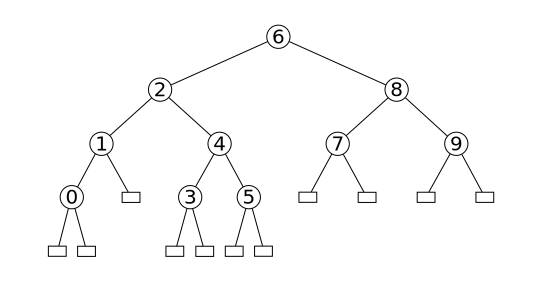
\includegraphics[width=\textwidth] {bin_search_tree.png}}
	\caption{Бинарное дерево поиска}
	\label{fig:bin_search_tree}
\end{figure}

Извлечём значения узлов в виде сортированного списка при помощи инфиксного
просмотра следующей функцией:

\begin{lstlisting}[language=OCaml]
# let rec list_of_tree = function
    Empty -> []
  | Node(lb, r, rb) -> (list_of_tree lb) @ (r :: (list_of_tree rb)) ;;
val list_of_tree : 'a arbre_bin -> 'a list = <fun>
\end{lstlisting}

Для того чтобы получить из списка бинарное дерево, определим функцию:

\begin{lstlisting}[language=OCaml]
# let rec ajout x = function
    Empty  ->  Node(Empty, x, Empty)
  | Node(fg, r, fd)  ->  if x < r then Node(ajout x fg, r, fd)
                         else Node(fg, r, ajout x fd) ;;
val ajout : 'a -> 'a arbre_bin -> 'a arbre_bin = <fun>
\end{lstlisting}

Функция трансформирующая список в бинарное дерево может быть получена
использованием функции \texttt{ajout}

\begin{lstlisting}[language=OCaml]
# let rec arbre_of_list = function
      []   ->  Empty
   | t::q  ->  ajout t (arbre_of_list q)  ;;
val arbre_of_list : 'a list -> 'a arbre_bin = <fun>
\end{lstlisting}

Тогда функция сортировки это всего--навсего композиция функций
\texttt{arbre\_of\_list} и \texttt{list\_of\_arbre}.

\begin{lstlisting}[language=OCaml]
# let tri x = list_of_arbre (arbre_of_list x) ;;
val tri : 'a list -> 'a list = <fun>
# tri [5; 8; 2; 7; 1; 0; 3; 6; 9; 4] ;;
- : int list = [0; 1; 2; 3; 4; 5; 6; 7; 8; 9]
\end{lstlisting}

\subsubsection{Общие планарные деревья}

Воспользуемся функцией определённой в модуле List (см. \ref{??}):

\begin{itemize}
	\item \texttt{List.map}: которая применяет одну функцию ко всем элементам
списка и возвращает список результатов.

	\item \texttt{List.fold\_left}: эквивалент функции \texttt{fold\_left}
определённой на стр. \ref{sec:caml_kernel:examples:lstlisting}

	\item \texttt{List.exists} применяет функцию булевого значения ко всем
элементам и если одно из применений возвращает \texttt{true}, то результат
\texttt{true}, иначе \texttt{false}. 
\end{itemize}

Общее планарное дерево --- это дерево в котором нет ограничения на число
дочерних узлов: каждому узлу ассоциируем список дочерних узлов и длина этого
списка не ограничена.

\begin{lstlisting}[language=OCaml]
# type 'a arbre = Empty
               | Node of 'a * 'a arbre list ;;
type 'a arbre = Empty | Node of 'a * 'a arbre list
\end{lstlisting}

Пустое дерево представлено значением \texttt{Empty}, лист --- это узел без
дочерних узлов формы \texttt{Node(х,[])} или \texttt{Node(x, [
Empty ; Empty; .. ])}. Таким образом достаточно просто написать функции,
манипулирующие подобными деревьями такие как принадлежность элемента дереву или
вычисление высоты дерева.

Для проверки принадлежности элемента \texttt{e} воспользуемся следующим
алгоритмом: если дерево пустое, тогда элемент \texttt{e} не принадлежит этому
дереву, в противном случае \texttt{e} принадлежит дереву только если он равен
значению корня дерева или принадлежит дочерним узлам.

\begin{lstlisting}[language=OCaml]
val belongs : 'a -> 'a arbre -> bool = <fun>
# let rec appartient e = function
    Empty -> false
  | Node(v, fs) -> (e=v) or (List.exists (appartient e) fs) ;;
val appartient : 'a -> 'a arbre -> bool = <fun>
\end{lstlisting}

Для вычисления высоты дерева, напишем следующую функцию: высота пустого дерева
равна 0, в противном случае его высота равна высоте самого большого под--дерева
плюс 1.

\begin{lstlisting}[language=OCaml]
# let rec hauteur =
  let max_list l = List.fold_left max 0 l in
   function
     Empty -> 0
   | Node (_, fs) -> 1 + (max_list (List.map hauteur fs)) ;;
val hauteur : 'a arbre -> int = <fun>
\end{lstlisting}

\subsection{Не функциональные рекурсивные значения}

Рекурсивное объявление не функциональных значений позволяет конструировать
циклические структуры данных.

Следующее объявление создаёт циклический список одного элемента.

\begin{lstlisting}[language=OCaml]
# let rec l = 1::l ;;
val l : int list =
  [1; 1; 1; 1; 1; 1; 1; 1; 1; 1; 1; 1; 1; 1; 1; 1; 1; 1; 1; 1; 1; 1; 1; 1; 1;
   1; 1; 1; 1; 1; 1; 1; 1; 1; 1; 1; 1; 1; 1; 1; 1; 1; 1; 1; 1; 1; 1; 1; 1; 1;
   1; 1; 1; 1; 1; 1; 1; 1; 1; 1; 1; 1; 1; 1; 1; 1; 1; 1; 1; 1; 1; 1; 1; 1; 1;
   1; 1; 1; 1; 1; 1; 1; 1; 1; 1; 1; 1; 1; 1; 1; 1; 1; 1; 1; 1; 1; 1; 1; 1; 1;
   1; 1; 1; 1; 1; 1; 1; 1; 1; 1; 1; 1; 1; 1; 1; 1; 1; 1; 1; 1; 1; 1; 1; 1; 1;
   1; 1; 1; 1; 1; 1; 1; 1; 1; 1; 1; 1; 1; 1; 1; 1; 1; 1; 1; 1; 1; 1; 1; 1; 1;
   1; 1; 1; 1; 1; 1; 1; 1; 1; 1; 1; 1; 1; 1; 1; 1; 1; 1; 1; 1; 1; 1; 1; 1; 1;
   1; 1; 1; 1; 1; 1; 1; 1; 1; 1; 1; 1; 1; 1; 1; 1; 1; 1; 1; 1; 1; 1; 1; 1; 1;
   1; 1; 1; 1; 1; 1; 1; 1; 1; 1; 1; 1; 1; 1; 1; 1; 1; 1; 1; 1; 1; 1; 1; 1; 1;
   1; 1; 1; 1; 1; 1; 1; 1; 1; 1; 1; 1; 1; 1; 1; 1; 1; 1; 1; 1; 1; 1; 1; 1; 1;
   1; 1; 1; 1; 1; 1; 1; 1; 1; 1; 1; 1; 1; 1; 1; 1; 1; 1; 1; 1; 1; 1; 1; 1; 1;
   1; 1; 1; 1; 1; 1; 1; 1; 1; 1; 1; 1; 1; 1; 1; 1; 1; 1; 1; 1; 1; 1; 1; 1;
   ...]
\end{lstlisting}

Применение рекурсивной функции к подобному списку приведет к переполнению
памяти.

\begin{lstlisting}[language=OCaml]
# size l ;;
Stack overflow during evaluation (looping recursion?).
\end{lstlisting}

Структурное равенство таких списков может быть проверенно лишь в случае, когда
физическое равенство верно.

\begin{lstlisting}[language=OCaml]
l=l ;;
- : bool = true
\end{lstlisting}

В случае, если мы определим такой же новый список, не стоит использовать
проверку на структурное равенство, под угрозой зацикливания программы. Таким
образом следующая инструкция не рекомендуется.

\begin{lstlisting}[language=OCaml]
let rec l2 = 1::l2 in l=l2 ;;
\end{lstlisting}

Однако, физическое равенство остаётся возможным.

\begin{lstlisting}[language=OCaml]
# let rec l2 = 1::l2 in l==l2 ;;
- : bool = false
\end{lstlisting}

Предикат \texttt{==} сравнивает непосредственно значение или разделения
структурного объекта (одним словом равенство по адресу). Мы воспользуемся этим
тестом для того чтобы при просмотре списка, не проверять уже просмотренные
под-списки. Сначала, определим функцию \texttt{memq} которая проверяет
присутствие элемента в списке при помощи физического равенства. В это же время
функция \texttt{mem} проверяет равенство структурное. Обе функции принадлежат
модулю \texttt{List}.

\begin{lstlisting}[language=OCaml]
# let rec memq a l = match l with
     [] -> false
   | b::l -> (a==b) or (memq a l) ;;
val memq : 'a -> 'a list -> bool = <fun>
\end{lstlisting}

Функция вычисляющая размер списка определена при помощи списка уже проверенных
списков и останавливается при встрече списка второй раз.

\begin{lstlisting}[language=OCaml]
# let special_size l =
   let rec size_aux previous l = match l with
       [] -> 0
     |  _::l1  -> if memq  l previous then 0
                       else 1 + (size_aux (l::previous) l1)
   in size_aux [] l ;;
val special_size : 'a list -> int = <fun>
# special_size [1;2;3;4] ;;
- : int = 4
# special_size l ;;
- : int = 1
# let rec l1 = 1::2::l2  and  l2 = 1::2::l1 in special_size l1 ;;
- : int = 4
\end{lstlisting}




\section{Типизация, область определения и исключения}
\label{sec:typing_domain_of_definition_and_exceptions}

Вычисленный тип функции принадлежит подмножеству множества в котором она
определена. Если входной аргумент функции типа \texttt{int}, это не значит что
она сможет быть выполнена для любого переданного ей целого числа. Таких случаях
мы используем механизм исключений Objective CAML. Запуск исключения провоцирует
остановку вычислений, которое может быть выявлено и обработано. Для этого
необходимо установить обработчик исключения, до того как исключение может быть
возбуждено.

\subsection{Частичные функции и исключения}

Область определения функции соответствует множеству значений которыми функция
манипулирует. Существует множество математических частичных функций, таких как
например, деление или натуральный логарифм. Проблемы возникают в том случае,
когда функция манипулирует более сложными структурами данных. Действительно,
каков будет результат функции определяющей первый элемент списка, если список
пуст. Аналогично, вычисление факториала для отрицательного числа приводит к
бесконечному вычислению.

Определённое число исключительных ситуаций может произойти во время выполнения
программы, как например деление на ноль. Попытка деления на ноль может привести
в лучшем случае к остановке программы и в худшем к неправильному (некоэрантному)
состоянию машины. Безопасность языка программирования заключается в гарантии
того, что такие случаи не возникнут. Исключение есть один из способов такой
гарантии.

Деление 1 на 0 провоцирует запуск специального исключения:

\begin{lstlisting}[language=OCaml]
# 1/0;;
Exception: Division_by_zero.
\end{lstlisting}

Сообщение \texttt{Exception: Division\_by\_zero} указывает во первых на то, что
исключение\texttt{ Division\_by\_zero} возбуждено и во вторых, что оно не было
обработано.

Часто, тип функции не соответствует области ее определения в том случае когда
сопоставление с образцом не является полным, то есть когда он не отслеживает все
возможные случаи. Чтобы избежать такой ситуации, Objective CAML выводит
следующее сообщение.

\begin{lstlisting}[language=OCaml]
# let tete l = match l with t::q -> t ;;
Warning 8: this pattern-matching is not exhaustive.
Here is an example of a value that is not matched:
[]
val tete : 'a list -> 'a = <fun>
\end{lstlisting}

Однако, если программист все таки настаивает на своей версии, то Objective CAML
воспользуется механизмом исключения в случае неправильного вызова частичной
функции.

\begin{lstlisting}[language=OCaml]
# tete [] ;;
Exception: Match_failure ("", 9, 9).
\end{lstlisting}

Мы уже встречали другое исключение определенное в Objective CAML:
\texttt{Failure}, с входным аргументом типа \texttt{string}. Запустить это
исключение можно функцией \texttt{failwith}. Воспользуемся этим и дополним
определение функции \texttt{tete}.

\subsection{Определения исключения}

В Objective CAML, тип исключений --- \texttt{exn}. Это особенный тип ---
расширяемая сумма: мы можем увеличить множество значений этого типа объявляя
новые конструкторы. Такая особенность позволяет программисту определять свои
собственные исключения.

Синтаксис объявления следующий:

Синтаксис:

\begin{lstlisting}[language=OCaml]
exception Nom ;;
\end{lstlisting}

Синтаксис:

\begin{lstlisting}[language=OCaml]
exception Nom of t ;;
\end{lstlisting}

Вот несколько примеров объявления исключений.

\begin{lstlisting}[language=OCaml]
# exception A_MOI;;
exception A_MOI
# A_MOI;;
- : exn = A_MOI
# exception Depth of int;;
exception Depth of int
# Depth 4;;
- : exn = Depth 4
\end{lstlisting}

Имена исключений являются конструкторами --- это значит они должны начинаться с
заглавной буквы.

\begin{lstlisting}[language=OCaml]
# exception minuscule ;;
Error: Syntax error
\end{lstlisting}

{\it Предупреждение}

Исключения мономорфны, при объявлении типа аргумента мы не можем указать
параметризующий тип.

\begin{lstlisting}[language=OCaml]
exception Value of 'a ;;
Error: Unbound type parameter 'a
\end{lstlisting}

Полиморфное исключение позволило бы определение функций, возвращающих результат
любого типа. Подобный пример мы рассмотрим далее на \ref{}.

\subsection{Возбуждение исключения}

\texttt{raise} --- функциональный примитив языка Objective CAML, её входной
аргумент есть исключение, а возвращает он полиморфный тип.

\begin{lstlisting}[language=OCaml]
# raise ;;
- : exn -> 'a = <fun>
# raise A_MOI;;
Exception: A_MOI.
# 1+(raise A_MOI);;
Exception: A_MOI.
# raise (Depth 4);;
Exception: Depth 4.
\end{lstlisting}

В Objective CAML нет возможности написать функцию \texttt{raise}, она должна
быть определена системой.

\subsection{Перехват исключения}

Весь интерес возбуждения исключений содержится в возможности их обработать и
изменить выполнение программы в зависимости от этого исключения. В этом случае,
порядок вычисления выражения имеет значение для того чтобы определить какое
исключения было запущенно. Таким образом мы выходим из рамок чисто
функционального программирования, потому как порядок вычисления аргументов может
изменить результат. Об этом мы поговорим в следующей главе (стр. \ref{??})

Следующая конструкция, вычисляющая значение какого--то выражения, отлавливает
исключение, возбуждённое во время этого вычисления.

Синтаксис:

\begin{lstlisting}[language=OCaml]
try expr with
  | p1 -> expr1
  :
  | pn -> exprn
\end{lstlisting}

Если вычисление \texttt{expr} не возбудит исключения, то тип результата будет
типом подсчитываемым этим выражением. Иначе, в приведённом выше сопоставлении
будет искаться ответвление соответствующее этому исключению и будет возвращено
значение следующего за ним выражения.

Если ни одно ответвление не соответствует исключению, то оно будет переправлено
до следующего обработчика \texttt{try--with} установленного в программе. Таким
образом сопоставление исключения всегда исчерпывающий. Подразумевается что
последний фильтр \texttt{|e->raise e}. Если ни одного обработчика не найдено в
программе, система сама займётся обработкой этого исключения и остановит
программу с выводом сообщения об ошибке.

Важно понимать разницу между вычислением исключения (то есть значение типа
\texttt{exn}) и его обработкой, которое приостанавливает вычисления. Исключение,
как и любой другой тип, может быть возвращено функцией.

\begin{lstlisting}[language=OCaml]
# let rendre x = Failure x ;;
val rendre : string -> exn = <fun>
# rendre "test" ;;
- : exn = Failure "test"
# let declencher x = raise (Failure x) ;;
val declencher : string -> 'a = <fun>
# declencher "test" ;;
Exception: Failure "test".
\end{lstlisting}

Как вы наверно заметили, функция \texttt{declencher} (запустить) не возвращает
значение типа \texttt{exn}, тогда как \texttt{rendre} (вернуть) возвращает.

\subsubsection{Вычисления с исключениями}

Кроме обработки не желаемых значений, исключения можно использовать для
оптимизации. Следующий пример реализует произведение всех элементов списка целых
чисел. Мы воспользуемся исключением для остановки просмотра списка если
обнаружим 0, который мы вернём как результат функции.

\begin{lstlisting}[language=OCaml]
# exception Found_zero ;;
exception Found_zero
# let rec mult_rec l = match l with
     [] -> 1
   | 0 :: _ -> raise Found_zero
   | n :: x -> n * (mult_rec x) ;;
val mult_rec : int list -> int = <fun>
# let mult_list l =
    try mult_rec l with Found_zero -> 0 ;;
val mult_list : int list -> int = <fun>
# mult_list [1;2;3;0;5;6] ;;
- : int = 0
\end{lstlisting}

Оставшиеся вычисления, то есть произведения элементов после встреченного нуля,
не выполняются. После встречи \texttt{raise}, вычисление вновь продолжится с
\texttt{with}.





\section{Полиморфизм и значения возвращаемые функциями}

Полиморфизм Objective CAML позволяет определить функции, тип возвращаемого
выражения которых конкретно не определён. Например:

\begin{lstlisting}[language=OCaml]
# let id x = x ;;
val id : 'a -> 'a = <fun>
\end{lstlisting}

Однако, возвращаемый тип \texttt{id} зависит от типа аргумента. Таким образом,
если мы применим функцию \texttt{id} к какому-нибудь аргументу, то механизм
вывода (определения) типа сможет реализовать переменную типа \texttt{'a}. Для
каждого частного использования тип функции \texttt{id} может быть определён.

Иначе, использование жёсткой статической типизации, которая обеспечивает
правильность выполнения, не будет иметь смысла. Функция с полностью
неопределённым типом как \texttt{'a->'b}, разрешит какое попало преобразование
типа, что привело бы к ошибке выполнения, так как физическое представление
значений не одно и то же.

\subsubsection{Очевидное противоречие}

Мы можем определить функции, которые возвращают значение, тип которого не
соответствует типу аргументов. Рассмотрим несколько примеров и проанализируем
почему это не противоречит жёсткой статической типизации.

Вот первый пример:

\begin{lstlisting}[language=OCaml]
# let f x = [] ;;
val f : 'a -> 'b list = <fun>
\end{lstlisting}

Эта функция конструирует полиморфные значения из любого типа.

\begin{lstlisting}[language=OCaml]
# f () ;;
- : 'a list = []
# f "n'importe quoi" ;;
- : 'a list = []
\end{lstlisting}

Однако, полученное значение не совсем является не определённым ---
подразумевается список. Таким образом она не может использоваться где попало.

Вот три примера функций типа \texttt{'a -> 'b}:

\begin{lstlisting}[language=OCaml]
# let rec f1 x = f1 x ;;
val f1 : 'a -> 'b = <fun>
# let f2 x = failwith "n'importe quoi" ;;
val f2 : 'a -> 'b = <fun>
# let f3 x = List.hd [] ;;
val f3 : 'a -> 'b = <fun>
\end{lstlisting}

Эти функции не являются \enq{опасными} в отношении правильности выполнения
программы, так как их невозможно использовать для конструкции значений: первая
зацикливается, две последние запускают исключение, которые останавливают
выполнение программы.

Чтобы не было возможности определить функции типа \texttt{'a -> 'b}, новые
конструкторы исключений не должны иметь аргументы типы которых содержат
переменную.

Если бы могли объявить полиморфное исключение \texttt{Poly\_exn} типа \texttt{'a
-> exn}, то тогда следующая функция была бы возможна:

\begin{lstlisting}[language=OCaml]
let f = function
   0 -> raise (Poly_exn false)
 | n -> n+1 ;;
\end{lstlisting}

Таким образом, тип функции \texttt{f} это \texttt{int->int} и тип
\texttt{Poly\_exn} это \texttt{'a -> exn}, теперь напишем следующее:

\begin{lstlisting}[language=OCaml]
let g n = try f n with Poly_exn x -> x+1 ;;
\end{lstlisting}

Это правильно типизированная функция (поскольку аргумент \texttt{Poly\_exn}
может быть каким угодно) и вызов \texttt{g 0} попытается сложить целое с булевым
значением!



\section{Калькулятор}
\label{sec:desktop_calculator}

Для того чтобы понять как организуются программы на Objective CAML, необходимо
самим реализовать такую программу. Напишем калькулятор манипулирующий целыми
числами при помощи 4 стандартных операций.

Для начала, определим тип \texttt{key}, для представления кнопки калькулятора.
Всего таких кнопок будет 15: по одной для каждой операции, для каждой цифры и
для кнопки равно.

\begin{lstlisting}[language=OCaml]
# type key = Plus | Minus | Times | Div | Equals | Digit of int ;;
\end{lstlisting}

Заметим, что цифровые кнопки сгруппированы под одним конструктором
\texttt{Digit} с аргументом целого типа. Таким образом, некоторые значения типа
\texttt{key} не являются на самом деле кнопкой. Например, (\texttt{Digit 32})
есть значение типа \texttt{key}, но не представляет ни одну кнопку калькулятора.

Напишем функцию \texttt{valid} которая проверяет входной аргумент на
принадлежность к типу \texttt{key}. Тип функции \texttt{key->bool}.

На первом этапе определим функцию проверяющую что число принадлежит интервалу
0-9. Объявим её с именем \texttt{is\_digit}.

\begin{lstlisting}[language=OCaml]
# let est_chiffre = function x -> (x>=0) && (x<=9) ;;
val est_chiffre : int -> bool = <fun>
\end{lstlisting}

Теперь функция \texttt{valid} фильтрующая свой аргумент тип которого
\texttt{key}:

\begin{lstlisting}[language=OCaml]
let valide tch = match tch with
     Chiffre n -> est_chiffre n
   | _ -> true ;;
val valide : touche -> bool = <fun>
\end{lstlisting}

Первый фильтр применяется в случае если входной аргумент построен конструктором
\texttt{Digit}, в этом случае он проверяется функцией \texttt{is\_digit}. Второй
фильтр применяется в любом другом случае. Напомним, что благодаря фильтру, тип
фильтруемого значения обязательно будет \texttt{key}.

Перед тем как начать реализовывать алгоритм калькулятора, определим модель
формально описывающую реакцию на нажатие кнопок. Мы подразумеваем что
калькулятор располагает памятью в которой хранится результат последней операции,
последняя нажатая кнопка, последний использованный оператор и число выведенное
на экран. Все эти 4 значения назовем состоянием калькулятора, оно изменяется
каждый раз при нажатии на одну из кнопок. Это изменение называется переходом, а
теория управляющая подобным механизмом есть теория автоматов.

Состояние представлено следующим типом:

\begin{lstlisting}[language=OCaml]
type etat = {
   dce : int;    (* dernier calcul effectué     *)
   dta : touche; (* dernière touche actionnée   *)
   doa : touche; (* dernier opérateur actionné  *)
   vaf : int     (* valeur affichée             *)
 } ;;
\end{lstlisting}

В таблице \ref{tbl:transitions_for_3+21*2=} приведён пример состояний
калькулятора.

\begin{table}[hl]
\begin{center}
	\caption{Переходы 3+21*2=}
	\begin{tabular}{|c|c|c|}
	\hline
	 & Состояние & Значение \\
	\hline
	 & $(0, =, =, 0)$ & 3 \\
	\hline
	$\to$ & $(0, 3, =, 3)$ & + \\
	\hline
	$\to$ & $(3, +, +, 3)$ & 2 \\
	\hline
	$\to$ & $(3, 2, +, 2)$ & 1 \\
	\hline
	$\to$ & $(3, 1, +, 21)$ & * \\
	\hline
	$\to$ & $(24, *, *, 24)$ & 2 \\
	\hline
	$\to$ & $(24, 2, *, 2)$ & = \\
	\hline
	$\to$ & $(48, =, =, 48)$ & \\
	\hline
	\end{tabular}
\end{center}
	\label{tbl:transitions_for_3+21*2=}
\end{table}

Нам нужна функция \texttt{evaluate} с тремя аргументами: двумя операндами и
оператором, она возвращает результат операции. Для этого функция фильтрует
входной аргумент типа \texttt{key}:

\begin{lstlisting}[language=OCaml]
# let evalue x y tch = match tch with
     Plus  -> x + y
   | Moins -> x - y
   | Fois  -> x * y
   | Par   -> x / y
   | Egal  -> y
   | Chiffre _ -> failwith "evalue : no op";;
val evalue : int -> int -> touche -> int = <fun>
\end{lstlisting}

Дадим определение переходам, перечисляя все возможные случаи. Предположим, что
текущее состояние есть квадри--плет \texttt{(a, b, A, d)}:

\begin{itemize}
	\item кнопка с цифрой x нажата, есть два возможных случая:

	\begin{itemize}
		\item предыдущая нажатая кнопка тоже цифра, значит пользователь
продолжает	набирать число и необходимо добавить \texttt{x} к значению
выводимому на экран	то есть изменить его на \texttt{d * 10 + x}. Новое состояние
будет:	\texttt{(a,(Digit x), A, d * 10 + x)}

		\item предыдущая нажатая кнопка не цифра, тогда мы только начинаем
писать	новое число. Новое состояние: \texttt{(a, (Digit x), A, x)}
	\end{itemize}

	\item кнопка с оператором B была нажата, значит второй операнд был полностью
введён и теперь мы хотим \enq{что-то} сделать с двумя операндами. Для этого
сохранена последняя операция (\texttt{А}). Новое состояние: \texttt{(A d,B,B,a A
d)}
\end{itemize}

Для того чтобы написать функцию \texttt{transition}, достаточно дословно
перевести в Objective CAML предыдущее описание при помощи сопоставления входного
аргумента. Кнопку с двумя значениями обработаем локальной функцией
\texttt{digit\_transition} при помощи сопоставления.

\begin{lstlisting}[language=OCaml]
# let transition et tou =
   let transition_chiffre n = function
       Chiffre _  ->  { et with dta=tou; vaf=et.vaf*10+n }
     |  _         ->  { et with dta=tou; vaf=n }
   in
      match tou with
          Chiffre p  ->  transition_chiffre p et.dta
        |  _         ->  let res = evalue et.dce et.vaf et.doa
                         in { dce=res; dta=tou; doa=tou; vaf=res }  ;;
val transition : etat -> touche -> etat = <fun>
\end{lstlisting}

Эта функция из \texttt{state} и \texttt{key} считает новое состояние
\texttt{state}.

Протестируем теперь программу:

\begin{lstlisting}[language=OCaml]
# let etat_initial = { dce=0; dta=Egal; doa=Egal; vaf=0 } ;;
val etat_initial : etat = {dce=0; dta=Egal; doa=Egal; vaf=0}
# let etat2 = transition etat_initial (Chiffre 3) ;;
val etat2 : etat = {dce=0; dta=Chiffre 3; doa=Egal; vaf=3}
# let etat3 = transition etat2 Plus ;;
val etat3 : etat = {dce=3; dta=Plus; doa=Plus; vaf=3}
# let etat4 = transition etat3 (Chiffre 2) ;;
val etat4 : etat = {dce=3; dta=Chiffre 2; doa=Plus; vaf=2}
# let etat5 = transition etat4 (Chiffre 1) ;;
val etat5 : etat = {dce=3; dta=Chiffre 1; doa=Plus; vaf=21}
# let etat6 = transition etat5 Fois ;;
val etat6 : etat = {dce=24; dta=Fois; doa=Fois; vaf=24}
# let etat7 = transition etat6 (Chiffre 2) ;;
val etat7 : etat = {dce=24; dta=Chiffre 2; doa=Fois; vaf=2}
# let etat8 = transition etat7 Egal ;;
val etat8 : etat = {dce=48; dta=Egal; doa=Egal; vaf=48}
\end{lstlisting}

Мы можем сделать тоже самое, передав список переходов.

\begin{lstlisting}[language=OCaml]
# let transition_liste et lt = List.fold_left transition et lt ;;
val transition_liste : etat -> touche list -> etat = <fun>
# let exemple = [ Chiffre 3; Plus; Chiffre 2; Chiffre 1; Fois; Chiffre 2; Egal ]
 in transition_liste etat_initial exemple ;;
- : etat = {dce=48; dta=Egal; doa=Egal; vaf=48}
\end{lstlisting}




\section{Exercises}

\section{Резюме}

В этой главе мы изучили основы функционального программирования и
параметризованный полиморфизм, что вместе являются основными характеристиками
Objective CAML. Также мы описали синтаксис функциональной части ядра и типов.
Это дало нам возможность написать первые программы. Так же мы подчеркнули
глубокую разницу между типом функции и областью её применения. Механизм
исключений позволяет решить эту проблему, и в то же время вводит новый стиль
программирования, где мы явно указываем манеру вычисления.

\section{To learn more}
\label{sec:to_learn_more_2}
\chapter{Императивное программирование}

\chapter{Функциональный и императивный стиль}

\section{Введение}

Языки функционального и императивного программирования различаются контролем
выполнения программы и управлением памятью.

\begin{itemize}
	\item функциональная программа вычисляет выражение, в следствии чего мы
получаем некоторый результат. Порядок в котором выполнены операции расчёта и
физическое представление данных не влияют на результат, он одинаков во всех
случаях. При таком порядке вычислений, сбор памяти в Objective CAML неявно
осуществляется вызовом автоматического сборщика мусора или Garbage Collector
(GC) (см. главу \ref{??}).

	\item императивная программа это список инструкций изменяющих состояние
памяти. Каждый этап выполнения строго определён структурами контроля,
указывающими на следующую инструкцию. Такие программы чаще всего манипулируют
указателями на значение, чем самими значениями. Отсюда необходимость явного
выделения и освобождения памяти, что может порой приводить к ошибкам доступа к
памяти, однако ничто не запрещает использование GC.
\end{itemize}

Императивные языки предоставляют больший контроль над выполнением программы и
памятью. Находясь ближе к реальной машине, такой код может быть эффективнее, но
при этом код теряет в устойчивости выполнения. Функциональное программирование
предоставляет более высокий уровень абстракции и таким образом лучший уровень
устойчивости выполнения: типизация (динамическая или статическая) помогает
избежать некорректных значений, автоматическая сборка мусора, хотя и замедляет
скорость выполнения, обеспечивает правильное манипулирование областями памяти.

Исторически обе эти парадигмы программирования существовали в разных сферах:
символьные программы для первого случая и числовые для второго. Однако, с тех
времён кое--что изменилось, в частности появилась техника компиляции
функциональных языков и выросла эффективность GC. С другой стороны, устойчивость
выполнения стала важным критерием, иногда даже важнейшим критерием качества
программного обеспечения. В подтверждение этому \enq{коммерческий аргумент}
языка Java: эффективность не должна преобладать над правильностью, оставаясь при
этом благоразумно хорошей. Эта идея приобретает с каждым днем новых сторонников
в мире производителей программного обеспечения.

Objective CAML придерживается этой позиции: он объединяет обе парадигмы,
расширяя таким образом область своего применения и облегчая написание алгоритмов
в том или ином стиле. Он сохраняет, однако, хорошие свойства правильности
выполнения благодаря статической типизации, GC и механизму исключений.
Исключения — это первая структура контроля выполнения позволяющая
приостановить/продолжить расчёт при возникновении определённых условий. Эта
особенность находится на границе двух стилей программирования, хоть она и не
изменяет результат, но может изменить порядок вычислений. Введение физически
изменяемых значений может повлиять на чисто функциональную часть языка. Порядок
вычисления аргументов функции становится определимым если это вычисление
производит побочный эффект. По этим причинам подобные языки называются “не
чистые функциональные языки”. Мы теряем часть абстракции, так как программист
должен учитывать модель памяти и выполнение программы. Это не всегда плохо, в
частности для читаемости кода. Однако, императивные особенности изменяют систему
типов языка: некоторые функциональные программы, с теоретически правильными
типами, не являются правильными на практике из-за введения ссылок (reference).
Хотя такие программы могут быть легко переписаны.
\section{План главы}
\label{sec:plan_of_the_chapter_4}

В этой главе мы сравним функциональную и императивную модель Objective CAML по
критерию контроля выполнения программы и представления значений в памяти. Смесь
обоих стилей позволяет конструировать новые структуры данных. Это будет
рассмотрено в первом разделе. Во втором разделе мы обсудим выбор между
композицией функций (composition of functions) или последовательности
(sequencing) с одной стороны и разделение (sharing) или копирование значений с
другой. Третий раздел выявляет интерес к смешиванию двух стилей для создания
функциональных изменяемых данных (mutable functional data), что позволит
создавать не полностью вычисленные (evaluated) данные. В четвёртом разделе
рассмотрены streams, потенциально бесконечные потоки данных и их интеграция,
посредством сопоставления с образцом.

\section{Сравнение между функциональным и императивным стилями}
\label{sec:comparison_between_functional_and_imperative}

Воспользуемся строками (\texttt{string}) и списками (\texttt{'a list}) для
иллюстрации разницы между двумя стилями.

\subsection{С функциональной стороны}
\label{subsec:the_functional_side}

\texttt{map} это одна из классических функций в среде функциональных языков. В
чистом функциональном стиле она пишется так:

\begin{lstlisting}[language=OCaml]
# let rec map f l = match l with
      []   ->  []
   | h::q  ->  (f h) :: (map f q)  ;;
val map : ('a -> 'b) -> 'a list -> 'b list = <fun>
\end{lstlisting}

Конечный список состоит из результатов применения функции \texttt{f} к элементам
списка переданного в аргументе. Он рекурсивно создаётся указывая начальный
элемент (заголовок) (\texttt{f t}) и последующую часть (хвост) (\texttt{map f
q}). В частности, программа не указывает какой из них будет вычислен первым.

При этом, для написания такой функции программисту не нужно знать физическое
представление данных. Проблемы выделения памяти и разделения данных решаются
Objective CAML без внешнего вмешательства программиста. Следующий пример
иллюстрирует это:

\begin{lstlisting}[language=OCaml]
# let example = [ "one" ; "two" ; "three" ] ;;
val example : string list = ["one"; "two"; "three"]
# let result = map (function x -> x) example  ;;
val result : string list = ["one"; "two"; "three"]
\end{lstlisting}

Оба списка \texttt{example} и \texttt{result} содержат одинаковые значения:

\begin{lstlisting}[language=OCaml]
# example = result ;;
- : bool = true
\end{lstlisting}

Оба значения имеют одинаковую структуру, хоть они и представлены в памяти по
разному. Убедимся в этом при помощи проверки на физическое равенство:

\begin{lstlisting}[language=OCaml]
# example == result ;;
- : bool = false
# (List.tl example) == (List.tl result) ;;
- : bool = false
\end{lstlisting}

\subsection{Императивная сторона}
\label{subsec:the_imperative_side}

Вернёмся к предыдущему примеру и изменим строку списка \texttt{result}.

\begin{lstlisting}[language=OCaml]
# (List.hd result).[1] <- 's' ;;
- : unit = ()
# result ;;
- : string list = ["ose"; "two"; "three"]
# example ;;
- : string list = ["ose"; "two"; "three"]
\end{lstlisting}

Определено, изменив список \texttt{result}, мы изменили список \texttt{example}.
То есть знание физической структуры необходимо как только мы пользуемся
императивными особенностями.

Рассмотрим теперь как порядок вычисления аргументов функции может стать ловушкой
в императивном программировании. Определим структуру изменяемого списка, а так
же функции создания, добавления и доступа:

\begin{lstlisting}[language=OCaml]
# type 'a ilist = { mutable c : 'a list } ;;
type 'a ilist = { mutable c : 'a list; }
# let icreate () = { c = [] }
 let iempty l = (l.c = [])
 let icons x y = y.c <- x::y.c ; y
 let ihd x = List.hd x.c
 let itl x = x.c <- List.tl x.c ; x ;;
val icreate : unit -> 'a ilist = <fun>
val iempty : 'a ilist -> bool = <fun>
val icons : 'a -> 'a ilist -> 'a ilist = <fun>
val ihd : 'a ilist -> 'a = <fun>
val itl : 'a ilist -> 'a ilist = <fun>
# let rec imap f l =
   if iempty l then icreate()
   else icons (f (ihd l))  (imap f (itl l)) ;;
val imap : ('a -> 'b) -> 'a ilist -> 'b ilist = <fun>
\end{lstlisting}

Несмотря на то что мы переняли общую структуру функции \texttt{map} предыдущего
параграфа, с \texttt{imap} мы получим другой результат:

\begin{lstlisting}[language=OCaml]
# let example = icons "one" (icons "two" (icons "three" (icreate()))) ;;
val example : string ilist = {c = ["one"; "two"; "three"]}
# imap (function x -> x) example ;;
Exception: Failure "hd".
\end{lstlisting}

В чем тут дело? Вычисление (\texttt{itl l}) произошло раньше чем (\texttt{ihd
l}) и в последней итерации \texttt{imap}, список \texttt{l} пустой в момент
обращения к его заголовку. Список \texttt{example} теперь пуст, хоть мы и не
получили никакого результата:

\begin{lstlisting}[language=OCaml]
# example ;;
- : string ilist = {c = []}
\end{lstlisting}

Проблема функции \texttt{imap} в недостаточном контроле смеси стилей
программирования: мы предоставили системе выбор порядка вычисления.
Переформулируем функцию \texttt{imap} явно указав порядок при помощи конструкции
\texttt{let .. in ..}

\begin{lstlisting}[language=OCaml]
# let rec imap f l =
   if iempty l then icreate()
   else let h = ihd l  in  icons (f h)  (imap f (itl l)) ;;
val imap : ('a -> 'b) -> 'a ilist -> 'b ilist = <fun>
# let example = icons "one" (icons "two" (icons "three" (icreate()))) ;;
val example : string ilist = {c = ["one"; "two"; "three"]}
# imap (function x -> x) example ;;
- : string ilist = {c = ["one"; "two"; "three"]}
\end{lstlisting}

Однако, начальный список опять утерян:

\begin{lstlisting}[language=OCaml]
# example ;;
- : string ilist = {c = []}
\end{lstlisting}

Использование оператора последовательности (\texttt{sequencing operator}) и
цикла есть другой способ явного указания порядка.

\begin{lstlisting}[language=OCaml]
# let imap f l =
     let l_res = icreate ()
     in while not (iempty l) do
          ignore (icons (f (ihd l)) l_res) ;
          ignore (itl l)
        done ;
        { l_res with c = List.rev l_res.c } ;;
Warning 23: this record is defined by a `with' expression,
but no fields are borrowed from the original.
val imap : ('a -> 'b) -> 'a ilist -> 'b ilist = <fun>
# let example = icons "one" (icons "two" (icons "three" (icreate()))) ;;
val example : string ilist = {c = ["one"; "two"; "three"]}
# imap (function x -> x) example ;;
- : string ilist = {c = ["one"; "two"; "three"]}
\end{lstlisting}

Присутствие \texttt{ignore} --- это факт того что нас интересует побочный эффект
функций над её аргументами, а не их (функций) результат. Так же было необходимо
выстроить в правильном порядке элементы результата (функцией \texttt{List.rev}).

\subsection{Рекурсия или итерация}
\label{subsec:recursive_or_iterative}

Часто ошибочно ассоциируют рекурсию с функциональным стилем и императивный с
итерацией. Чисто функциональная программа не может быть итеративной, так как
значение условия цикла не меняется никогда. Тогда как императивная программа
может быть рекурсивной: функция \texttt{imap} тому пример.

Значения аргументов функции хранятся во время её выполнения. Если она (функция)
вызовет другую функцию, то эта последняя сохранит и свои аргументы. Эти значения
хранятся в стеке выполнения. При возврате из функции эти значения извлечены из
стека. Зная что пространство памяти ограничено, мы можем дойти до её предела,
используя функцию с очень большой глубиной рекурсии. В подобных случаях
Objective CAML возбуждает исключение \texttt{Stack\_overflow}.

\begin{lstlisting}[language=OCaml]
# let rec succ n = if n = 0 then 1 else 1 + succ (n-1) ;;
val succ : int -> int = <fun>
# succ 100000 ;;
- : int = 100001
\end{lstlisting}

В итеративной версии место занимаемое функцией \texttt{succ\_iter} в стеке не
зависит от величины аргумента.

\begin{lstlisting}[language=OCaml]
# let succ_iter n =
   let i = ref 0 in
     for j=0 to n do incr i done ;
     !i ;;
val succ_iter : int -> int = <fun>
# succ_iter 100000 ;;
- : int = 100001
\end{lstlisting}

У следующей версии функции {\it a priori} аналогичная глубина рекурсии, однако
она успешно выполняется с тем же аргументом.

\begin{lstlisting}[language=OCaml]
# let succ_tr n =
   let rec succ_aux n accu =
     if n = 0 then accu  else succ_aux (n-1) (accu+1)
   in
     succ_aux 1 n ;;
val succ_tr : int -> int = <fun>
# succ_tr 100000 ;;
- : int = 100001
\end{lstlisting}

Данная функция имеет специальную форму рекурсивного вызова, так называемую
хвостовую рекурсию при которой результат вызова функции будет результатом
функции без дополнительных вычислений. Таким образом отпадает необходимость
хранить аргументы функции во время вычисления рекурсивного вызова. Если
Objective CAML распознал конечную рекурсивную функцию, то перед её вызовом
аргументы извлекаются из стека.

Распознание конечной рекурсии существует во многих языках, однако это свойство
просто необходимо функциональным языкам, где она естественно много используется.
\section{Какой стиль выбрать?}
\label{sec:which_style_to_choose}

Естественно, речь не идёт о \enq{священных} либо эстетических для каждого
понятиях, {\it a priori} не существует стиля красивее или лучше чем другой.
Однако, в зависимости от решаемой проблемы, один стиль может быть более
подходящим или более адаптированным чем другой.

Первое правило --- простота. Желаемый алгоритм (будь то в книге или лишь в
голове программиста) уже определён в каком-то стиле, вполне естественно его и
использовать при реализации.

Второй критерий --- эффективность программы. Можно сказать что императивная
программа (хорошо написанная) более эффективна чем её функциональный аналог, но
в очень многих случаях разница между ними не достаточно существенна для
оправдания сложности кода императивного стиля, там где функциональный был бы
естественен. Функция \texttt{map} есть хороший пример натурально выраженной в
функциональном стиле проблемы и мы ни в чем не выиграем написав её в
императивном стиле.

\subsection{Последовательность или композиция функций}
\label{subsec:sequence_or_composition_of_functions}

Мы уже видели, что как только в программе появляются побочные эффекты,
необходимо явно указывать порядок выполнения элементов программы. Это может быть
сделано двумя способами:

\begin{description}
	\item [функциональным] опираясь на то что Objective CAML строгий язык, то
есть аргумент вычислен до того как он будет передан функции. В выражение
\texttt{(f (g x))} сначала вычисляется \texttt{(g x)} и затем передача этого
результат функции \texttt{f}. В более сложных выражениях, промежуточный
результат может быть именован конструкцией \texttt{let in}, но принцип остаётся
тем же: \texttt{let aux=(g x) in (f aux)}.

	\item [императивный] используя последовательность или другую структуру
контроля (цикл). В этом случае, результатом будет побочный эффект над памятью, а
не значение возвращённое функцией : \texttt{aux:=(g x) ; (f!aux)}.
\end{description}

Давайте рассмотрим данную проблему выбора стиля на следующем примере.
Рекурсивный алгоритм быстрой сортировки вектора описывается следующим образом:

\begin{enumerate}
	\item выбрать опорную точку: выбрать индекс элемента в векторе

	\item переставить элементы вокруг этой точки: переставить элементы вектора
так чтобы значения меньше значения в опорной точке были слева от неё, а большие
значения справа

	\item отсортировать (тем же алгоритмом) два полученных вектора: элементы
после опорной точки и до неё
\end{enumerate}

Сортировка вектора --- означает изменение его состояния, поэтому мы должны
использовать императивный стиль, как минимум для манипуляции данными.

Начнём с определения функции переставляющей элементы вектора.

\begin{lstlisting}[language=OCaml]
# let permute_element vec n p =
   let aux = vec.(n) in vec.(n) <- vec.(p) ; vec.(p) <- aux  ;;
val permute_element : 'a array -> int -> int -> unit = <fun>
\end{lstlisting}

Выбор правильной точки опоры важен для эффективности алгоритма, но мы
ограничимся самым простым способом: вернём индекс первого элемента вектора.

\begin{lstlisting}[language=OCaml]
# let choose_pivot vec start finish = start ;;
val choose_pivot : 'a -> 'b -> 'c -> 'b = <fun>
\end{lstlisting}

Напишем теперь желаемый алгоритм переставляющий элементы вектора вокруг
выбранной точки.

\begin{itemize}
	\item установить опорную точку в начало вектора

	\item \texttt{i} индекс второго элемента вектора
	
	\item \texttt{j} индекс последнего элемента вектора
	
	\item если элемент с индексом \texttt{j} больше чем значение в опорной
точке, поменяем местами их значения и увеличим \texttt{i} на единицу, иначе
уменьшим \texttt{j} на единицу

	\item до тех пор пока \texttt{i} меньше чем \texttt{j} повторить предыдущую
операцию

	\item к этому этапу каждый элемент с индексом меньшим чем \texttt{i} (или
\texttt{}j) меньше значения в опорной точке, а остальные элементы больше: если
элемент с индекс \texttt{i} меньше чем опорное значение мы меняем их местами,
иначе меняем с предыдущим элементом.
\end{itemize}

При реализации алгоритма мы естественно воспользуемся императивными управляющими
структурами.

\begin{lstlisting}[language=OCaml]
# let permute_pivot vec start finish ind_pivot =
    permute_element vec start ind_pivot ;
    let i = ref (start+1) and j = ref finish and pivot = vec.(start) in
    while !i < !j do
      if vec.(!j) >= pivot then decr j
      else
        begin
          permute_element vec !i !j ;
          incr i
        end
    done ;
    if vec.(!i) > pivot then decr i ;
    permute_element vec start !i ;
    !i
 ;;
val permute_pivot : 'a array -> int -> int -> int -> int = <fun>
\end{lstlisting}

Кроме эффекта над вектором, функция возвращает индекс опорной точки.

Нам остаётся лишь собрать воедино различные этапы и написать рекурсивный вызов
для подвекторов.

\begin{lstlisting}[language=OCaml]
# let rec quick vec start finish =
    if start < finish
    then
      let pivot = choose_pivot vec start finish in
      let place_pivot = permute_pivot vec start finish pivot in
      quick (quick vec start (place_pivot-1)) (place_pivot+1) finish
    else vec ;;
val quick : 'a array -> int -> int -> 'a array = <fun>
\end{lstlisting}

Здесь мы воспользовались двумя стилями. Выбранная опорная точка служит
аргументом при перестановке вокруг неё и её порядок в векторе после этой
процедуры служит аргументом рекурсивного вызова. Зато, полученный после
перестановки вектор мы получаем в результате побочного эффекта, а не как
возвращённое значение функции \texttt{permute\_pivot}. Тогда как функция
\texttt{quick} возвращает вектор и сортировка подвекторов реализуется
композицией рекурсивных вызовов.

Теперь главная функция:

\begin{lstlisting}[language=OCaml]
# let quicksort vec = quick vec 0 ((Array.length vec)-1) ;;
val quicksort : 'a array -> 'a array = <fun>
\end{lstlisting}

Это полиморфная функция, так как отношение порядка < полиморфное.

\begin{lstlisting}[language=OCaml]
# let t1 = [|4;8;1;12;7;3;1;9|] ;;
val t1 : int array = [|4; 8; 1; 12; 7; 3; 1; 9|]
# quicksort t1 ;;
- : int array = [|1; 1; 3; 4; 7; 8; 9; 12|]
# t1 ;;
- : int array = [|1; 1; 3; 4; 7; 8; 9; 12|]
# let t2 = [|"the"; "little"; "cat"; "is"; "dead"|] ;;
val t2 : string array = [|"the"; "little"; "cat"; "is"; "dead"|]
# quicksort t2 ;;
- : string array = [|"cat"; "dead"; "is"; "little"; "the"|]
# t2 ;;
- : string array = [|"cat"; "dead"; "is"; "little"; "the"|]
\end{lstlisting}

\subsection{Общее использование или копии значений}
\label{subsec:shared_or_copy_values}

До тех пор пока наши данные не изменяемые, нет необходимости знать используются
они совместно или нет.

\begin{lstlisting}[language=OCaml]
# let id x = x ;;
val id : 'a -> 'a = <fun>
# let a = [ 1; 2; 3 ] ;;
val a : int list = [1; 2; 3]
# let b = id a ;;
val b : int list = [1; 2; 3]
\end{lstlisting}

Является ли \texttt{b} копией \texttt{a} или же это один и тот же список не
имеет значения, так как по любому это \enq{неосязаемые} значения. Однако, если
на место целых чисел, мы поместим изменяемые значения, необходимо будет знать
скажется ли изменение одного значения на другое.

Реализация полиморфизма Objective CAML вызывает (causes) копирование
непосредственных значений (immediate values) и разделение (sharing) структурных
значений. Хоть передача аргументов осуществляется копированием, в случае
структурных значений передается лишь указатель. Как в случае с функцией
\texttt{id}.

\begin{lstlisting}[language=OCaml]
# let a = [| 1 ; 2 ; 3 |] ;;
val a : int array = [|1; 2; 3|]
# let b = id a ;;
val b : int array = [|1; 2; 3|]
# a.(1) <- 4 ;;
- : unit = ()
# a ;;
- : int array = [|1; 4; 3|]
# b ;;
- : int array = [|1; 4; 3|]
\end{lstlisting}

Здесь мы действительно имеем случай выбора стиля программирования, от которого
зависит эффективность представления данных. С одной стороны, использование
изменяемых значений позволяет немедленное манипулирование данными (без
дополнительного выделения памяти). Однако это вынуждает, в некоторых случаях,
делать копии там, где использование неизменяемого значения позволило бы
разделение. Проиллюстрируем это двумя способами реализации списков.

\begin{lstlisting}[language=OCaml]
# type 'a list_immutable = LInil | LIcons of 'a * 'a list_immutable ;;
type 'a list_immutable = LInil | LIcons of 'a * 'a list_immutable
# type 'a list_mutable = LMnil | LMcons of 'a * 'a list_mutable ref ;;
type 'a list_mutable = LMnil | LMcons of 'a * 'a list_mutable ref
\end{lstlisting}

Фиксированные списки строго эквивалентны спискам Objective CAML, тогда как
изменяемые больше в стиле C, где ячейка состоит из значения и ссылки на
следующую ячейку.

С фиксированными списками существует единственный способ реализовать
конкатенацию и он вынуждает копирование структуры первого списка, тогда как
второй список может быть разделен с конечным списком.

\begin{lstlisting}[language=OCaml]
# let rec concat l1 l2 = match l1 with
     LInil -> l2
   | LIcons (a,l11) -> LIcons(a, (concat l11 l2)) ;;
val concat : 'a list_immutable -> 'a list_immutable -> 'a list_immutable =
  <fun>
# let li1 = LIcons(1, LIcons(2, LInil))
 and li2 =  LIcons(3, LIcons(4, LInil)) ;;
val li1 : int list_immutable = LIcons (1, LIcons (2, LInil))
val li2 : int list_immutable = LIcons (3, LIcons (4, LInil))
# let li3 = concat li1 li2 ;;
val li3 : int list_immutable =
  LIcons (1, LIcons (2, LIcons (3, LIcons (4, LInil))))
# li1==li3 ;;
- : bool = false
# let tlLI l =  match l with
   LInil       -> failwith "Liste vide"
 | LIcons(_,x) -> x ;;
val tlLI : 'a list_immutable -> 'a list_immutable = <fun>
# tlLI(tlLI(li3)) == li2 ;;
- : bool = true
\end{lstlisting}

В этом примере мы видим что первые ячейки \texttt{li1} и \texttt{li3} различны,
тогда как вторая часть \texttt{li3} есть именно \texttt{li2}.

С изменяемыми списками можно изменить аргументы (функция \texttt{concat\_share})
или создать новое значение (функция \texttt{concat\_copy})

\begin{lstlisting}[language=OCaml]
# let rec concat_copy l1 l2 =  match l1 with
     LMnil  -> l2
   | LMcons (x,l11) -> LMcons(x, ref (concat_copy !l11 l2)) ;;
val concat_copy : 'a list_mutable -> 'a list_mutable -> 'a list_mutable =
  <fun>
\end{lstlisting}

Это решение, \texttt{concat\_copy}, аналогично предыдущей функции
\texttt{concat}. Вот второе вариант, с общим использованием.

\begin{lstlisting}[language=OCaml]
# let concat_share l1 l2 =
  match l1 with
    LMnil -> l2
  | _     -> let rec set_last = function
                LMnil       -> failwith "concat_share : impossible case!!"
              | LMcons(_,l) -> if !l=LMnil then l:=l2 else set_last !l
             in
               set_last l1 ;
               l1 ;;
val concat_share : 'a list_mutable -> 'a list_mutable -> 'a list_mutable =
  <fun>
\end{lstlisting}

Конкатенация с общим использованием не нуждается в выделении памяти (мы не
используем конструктор \texttt{LMcons}), мы лишь ограничиваемся тем что
последняя ячейка первого списка теперь указывает на второй список. При этом,
конкатенация способна изменить аргументы переданные функции.

\begin{lstlisting}[language=OCaml]
# let lm1 = LMcons(1, ref (LMcons(2, ref LMnil)))
 and lm2 = LMcons(3, ref (LMcons(4, ref LMnil))) ;;
val lm1 : int list_mutable =
  LMcons (1, {contents = LMcons (2, {contents = LMnil})})
val lm2 : int list_mutable =
  LMcons (3, {contents = LMcons (4, {contents = LMnil})})
# let lm3 = concat_share lm1 lm2 ;;
val lm3 : int list_mutable =
  LMcons (1,
   {contents =
     LMcons (2,
      {contents = LMcons (3, {contents = LMcons (4, {contents = LMnil})})})})
\end{lstlisting}

Мы получили ожидаемый результат для \texttt{lm3}, однако значение \texttt{lm1}
изменено.

\begin{lstlisting}[language=OCaml]
# lm1 ;;
- : int list_mutable =
LMcons (1,
 {contents =
   LMcons (2,
    {contents = LMcons (3, {contents = LMcons (4, {contents = LMnil})})})})
\end{lstlisting}

Таким образом это может повлиять на оставшуюся часть программы.

\subsection{Критерии выбора}
\label{subsec:how_to_choose_your_style}

В чисто функциональной программе побочных эффектов не существует, это свойство
лишает нас операций ввода/вывода, исключений и изменяемых структур данных. Наше
определение функционального стиля является менее ограниченным, то есть функция
не изменяющая своё глобальное окружение может быть использована в функциональном
стиле. Подобная функция может иметь локальные изменяемые значения (и значит
следовать императивному стилю), но не должна изменять ни глобальные переменные
ни свои аргументы. С внешней стороны, такие функции можно рассматривать как
\enq{чёрный ящик}, чьё поведение сравнимо с поведением функции в чисто
функциональном стиле, с разницей что выполнение первой может быть приостановлен
возбуждением исключения. В том же духе, изменяемое значение, которое больше не
изменяется после инициализации, может быть использовано в функциональном стиле.

С другой стороны, программа написанная в императивном стиле, унаследует
следующие достоинства Objective CAML: правильность статической типизации,
автоматическое управление памятью, механизм исключений, параметризованный
полиморфизм и вывод типов.

Выбор между стилем функциональным и императивным зависит от программного
обеспечения которое вы хотите реализовать. Выбор может быть сделан в
соответствии со следующими характеристиками:

\begin{description}
	\item [выбор структур данных:] от использования или нет изменяемых структур
данных будет зависеть выбор стиля программирования. Действительно,
функциональный стиль по своей природе не совместим с изменением значений.
Однако, создание и просмотр значения не зависят от её свойств. Таким образом мы
возвращаемся к дискуссии \enq{изменение на месте vs копия} в
\ref{subsec:shared_or_copy_values}, к которой мы вернёмся для обсуждения
критерия эффективности.

	\item [структура данных существует:]
    если в программе необходимо менять изменяемые структуры данных (modify
mutable data structures), то императивный стиль является единственно возможным.
Однако, если необходимо лишь читать значения, то применение функционального
стиля гарантирует целостность данных. Использование рекурсивных структур данных
подразумевает рекурсивные функции, которые могут быть определены используя
особенности того или иного стиля программирования. Однако в общем случае бывает
проще истолковывать создание значения следуя рекуррентному определению. Этот
подход более близок к функциональному стилю, чем повторяющаяся обработка этого
значения рекурсией.

	\item [критерий эффективности:] немедленное изменение без сомнения лучше чем
создание значения. В случае когда эффективность кода является главенствующим
критерием, чаша весов перевешивает в сторону императивного стиля. Однако отметим
что совместное использование значений может оказаться нелёгкой задачей и в конце
концов более дорогостоящей, чем копирование значений с самого начала. Чистая
функциональность имеет определённую цену: частичное применение (partial
application) и использование функций переданных в виде аргумента другой функции
несёт более серьёзные накладные расходы в процессе выполнения программы, чем
явное применение видимой функции. Стоит избегать использования этой
функциональной особенности в тех местах, где критерий производительности
является решающим.

	\item [критерий разработки:] более высокий уровень абстракции
функционального стиля программирования позволяет более быстрое написание
компактного кода, содержащего меньше ошибок чем императивный вариант, который по
своей природе является более \enq{многословным}. Таким образом, функциональный
стиль является выгодным при разработке значительных программ. Независимость
функции к своему контексту окружения позволяет разделить код на более маленькие
части и тем самым облегчить его проверку и читаемость. Более высокая модульность
функционального стиля плюс возможность передавать функции (а значит и обработку)
в аргумент другим функциям повышает вероятность повторного использования
программ.
\end{description}

Эти несколько замечаний подтверждают тот факт, что часто смешанное использование
обоих стилей является рациональным выбором. Функциональный стиль быстрее в
разработке и обеспечивает более простую организацию программы, однако части кода
где необходимо повысить скорость выполнения лучше написать в императивном стиле.
\section{Смешивая стили}
\label{sec:mixing_styles}

Как мы уже заметили, язык программирования имеющий функциональные и
императивные особенности даёт свободу выбора наиболее подходящего стиля для
реализации того или иного алгоритма. Конечно, мы можем использовать оба аспекта
Objective CAML совместно в одной и той же функции. Именно этим мы сейчас и
займёмся.

\subsection{Замыкания и побочные эффекты}
\label{subsec:closures_and_side_effects}

Обычно функция с побочным эффектом рассматривается как процедура и она
возвращает значение () типа \texttt{unit}. Однако, иногда бывает полезно
произвести побочный эффект внутри функции и вернуть определённое значение. Мы
уже использовали подобный коктейль стилей в функции \texttt{permute\_pivot} в
быстрой сортировке.

В следующем примере реализуем генератор символов, который создаёт новый символ
при каждом вызове функции. Мы используем счётчик, значение которого
увеличивается с каждым вызовом.

\begin{lstlisting}[language=OCaml]
# let c = ref 0;;
val c : int ref = {contents = 0}
# let reset_symb = function () -> c:=0 ;;
val reset_symb : unit -> unit = <fun>
# let new_symb = function s ->  c:=!c+1 ; s^(string_of_int !c) ;;
val new_symb : string -> string = <fun>
# new_symb "VAR" ;;
- : string = "VAR1"
# new_symb "VAR" ;;
- : string = "VAR2"
# reset_symb () ;;
- : unit = ()
# new_symb "WAR" ;;
- : string = "WAR1"
# new_symb "WAR" ;;
- : string = "WAR2"
\end{lstlisting}

А теперь спрячем ссылку на c от всей программы следующим образом:

\begin{lstlisting}[language=OCaml]
# let (reset_s , new_s) =
   let c = ref 0
   in let f1 () = c := 0
      and f2 s  = c := !c+1 ; s^(string_of_int !c)
   in (f1,f2) ;;
val reset_s : unit -> unit = <fun>
val new_s : string -> string = <fun>
\end{lstlisting}

Таким образом мы объявили пару функций, разделяющие локальную (для декларации)
переменную \texttt{c}. Использование обеих функций производит тот же результат
что и раньше.

Этот пример иллюстрирует способ представления замыкания. Замыкание можно
рассматривать как пару, состоящую из кода (то есть часть \texttt{function}) и
локальное окружение, содержащее значения свободных переменных замыкания с другой
стороны. На диаграмме \ref{fig:memory_representation_of_closures} мы можем
увидеть представление в памяти замыканий \texttt{reset\_s} и \texttt{new\_s}.

\begin{figure}[h]
	\center{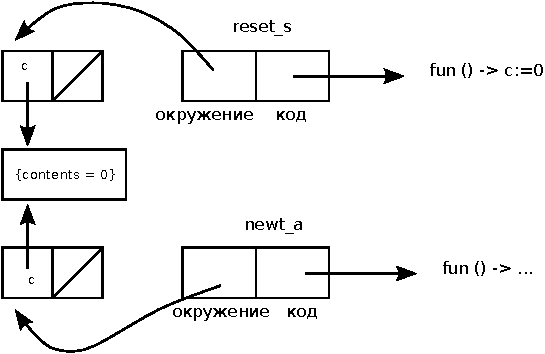
\includegraphics[width=\textwidth]
{img/memory_representation_of_closures}}
	\caption{\label{fig:memory_representation_of_closures}Представление в памяти 
замыканий}
\end{figure}

Оба эти замыкания разделяют одно и тоже окружение (значение \texttt{c}). Когда
одно из них меняет ссылку \texttt{c}, то оно меняет содержимое памяти
разделяемое с другим окружением.

\subsection{Физическое изменение и исключения}
\label{subsec:physical_modifications_and_exceptions}

 Исключения позволяет отслеживать ситуацию, при которой дальнейшее продолжение
программы невозможно. В подобном случае сборщик исключений позволит продолжить
вычисление, зная что произошла ошибка. В момент возбуждения исключения может
возникнуть проблема побочного эффекта с состоянием модифицируемых данных. Это
состояние не может быть гарантированно если произошли физические изменения в
ответвлении неудавшегося вычисления.

Определим функцию увеличения (++), с аналогичным результатом что и в C:

\begin{lstlisting}[language=OCaml]
# let (++) x = x:=!x+1; x;;
val ( ++ ) : int ref -> int ref = <fun>
\end{lstlisting}

Следующий пример, иллюстрирует небольшой расчёт в котором деление на ноль
совпадает с побочным эффектом:

\begin{lstlisting}[language=OCaml]
# let x = ref 2;;
val x : int ref = {contents = 2}
# !((++) x) * (1/0) ;;
Exception: Division_by_zero.
# x;;
- : int ref = {contents = 2}
# (1/0) * !((++) x) ;;
Exception: Division_by_zero.
# x;;
- : int ref = {contents = 3}
\end{lstlisting}

Переменная \texttt{x} не изменяется во время вычисления выражения (*1*), тогда
как она изменяется во время (*2*). Если заранее не сохранить начальные значения,
конструкция \texttt{try .. with ..} не должна (в части \texttt{with ..})
зависеть от изменяемых переменных, которые участвуют в вычислении возбудившем
исключение.

\subsection{Изменяемые функциональные структуры данных}
\label{subsec:modifiable_functional_data_structures}

В функциональном программирование программа, как функциональное выражение,
является в то же время данными --- чтобы уяснить этот момент напишем список
ассоциированных значений в виде функционального выражения. Этот список
ассоциаций \texttt{('a * 'b) list} можно рассматривать как частичную функцию из
\texttt{'a} (множество ключей) в \texttt{'b} (множество соответствующих
значений). Другими словами, функция \texttt{'a -> 'b}.

Пустой список это неопределённая функция, которую мы будем моделировать
возбуждением исключения:

\begin{lstlisting}[language=OCaml]
# let nil_assoc = function x -> raise Not_found ;;
val nil_assoc : 'a -> 'b = <fun>
\end{lstlisting}

Теперь напишем функцию \texttt{add\_assoc} добавляющую элемент в список или
другими словами расширим функцию новыми значениями.

\begin{lstlisting}[language=OCaml]
# let add_assoc (k,v) l = function x -> if x = k then v else l x ;;
val add_assoc : 'a * 'b -> ('a -> 'b) -> 'a -> 'b = <fun>
# let l = add_assoc ('1', 1) (add_assoc ('2', 2) nil_assoc) ;;
val l : char -> int = <fun>
# l '2' ;;
- : int = 2
# l 'x' ;;
Exception: Not_found.
\end{lstlisting}

Перепишем функцию \texttt{mem\_assoc}:

\begin{lstlisting}[language=OCaml]
# let mem_assoc k l = try  (l k) ; true  with  Not_found -> false ;;
val mem_assoc : 'a -> ('a -> 'b) -> bool = <fun>
# mem_assoc '2' l ;;
- : bool = true
# mem_assoc 'x' l ;;
- : bool = false
\end{lstlisting}

Однако, написание функции удаляющей элементы из списка, не совсем простое дело.
У нас больше нет доступа к значениям входящим в замыкание. Для этого мы спрячем
старое значение возбудив исключения \texttt{Not\_found}.

\begin{lstlisting}[language=OCaml]
# let rem_assoc k l = function x -> if x=k then raise Not_found else l x ;;
val rem_assoc : 'a -> ('a -> 'b) -> 'a -> 'b = <fun>
# let l = rem_assoc '2' l ;;
val l : char -> int = <fun>
# l '2' ;;
Exception: Not_found.
\end{lstlisting}

Естественно, можно воспользоваться ссылками и побочным эффектом для
использования таких значений, однако существует несколько предостережений.

\begin{lstlisting}[language=OCaml]
# let add_assoc_again (k,v) l =  l := (function x -> if x=k then v else !l x) ;;
val add_assoc_again : 'a * 'b -> ('a -> 'b) ref -> unit = <fun>
\end{lstlisting}

Мы получили функцию \texttt{l} которая указывает сама на саму себя и значит
будет зацикливаться. Этот досадный побочных эффект есть результат того что
разыменование \texttt{!l} находится внутри замыкания \texttt{function x ->}.
Значение \texttt{!l} вычислено при выполнении, а не компиляции. В этот момент,
\texttt{l} указывает на значение изменённое \texttt{add\_assoc}. Необходимо
исправить наше определение используя замыкание полученное определением
\texttt{add\_assoc}:

\begin{lstlisting}[language=OCaml]
# let add_assoc_again (k, v) l =  l := add_assoc (k, v) !l ;;
val add_assoc_again : 'a * 'b -> ('a -> 'b) ref -> unit = <fun>
# let l = ref nil_assoc ;;
val l : ('_a -> '_b) ref = {contents = <fun>}
# add_assoc_again ('1',1) l ;;
- : unit = ()
# add_assoc_again ('2',2) l ;;
- : unit = ()
# !l '1' ;;
- : int = 1
# !l 'x' ;;
Exception: Not_found.
\end{lstlisting}

\subsection{Ленивые изменяемые структуры}
\label{subsec:lazy_modifiable_data_structures}

Смесь императивных особенностей с функциональным языком образует хорошие
средства реализации языков программирования. В данном параграфе мы
проиллюстрируем эту особенность в реализации структур данных с отсроченным
вычислением. Такая структура данных не вычисляется полностью, вычисление
продвигается в зависимости от использования структуры.

Отложенное вычисление, часто используемое в чистых функциональных языках, можно
моделировать использованием функциональных значений (возможно, изменяемых).
Выгода от использования данных с отложенным выполнением двойная; во первых
вычисляется лишь то что необходимо для расчёта, во вторых использование
потенциально бесконечных данных.

Определим тип \texttt{vm} элементы которого либо уже вычисленное значение
(конструктор \texttt{Imm}) либо значение которое будет вычислено (конструктор
\texttt{Deferred}).

\begin{lstlisting}[language=OCaml]
# type 'a v =
     Imm of 'a
   | Deferred of (unit -> 'a);;
type 'a v = Imm of 'a | Deferred of (unit -> 'a)
# type 'a vm = {mutable c : 'a v };;
type 'a vm = { mutable c : 'a v; }
\end{lstlisting}

Откладывание вычислений может быть получено инкапсуляцией в замыкание. Функция
вычисляющая такое значение должна или вернуть значение если оно уже вычислено
или, в противном случае, вычислить и сохранить результат.

\begin{lstlisting}[language=OCaml]
# let eval e = match e.c with
   Imm a -> a
 | Deferred f -> let u = f () in e.c <- Imm u ; u ;;
val eval : 'a vm -> 'a = <fun>
\end{lstlisting}

Операции задержки и активации вычисления также называют замораживанием и
размораживанием значения.

Напишем условный контроль в виде функции:

\begin{lstlisting}[language=OCaml]
# let if_deferred c e1 e2 =
   if eval c then eval e1 else eval e2;;
val if_deferred : bool vm -> 'a vm -> 'a vm -> 'a = <fun>
\end{lstlisting}

А теперь воспользуемся этим в рекурсивной функции подсчёта факториала.

\begin{lstlisting}[language=OCaml]
# let rec facr n =
   if_deferred
          {c=Deferred(fun () -> n = 0)}
          {c=Deferred(fun () ->  1)}
          {c=Deferred(fun () -> n*(facr(n-1)))};;
val facr : int -> int = <fun>
# facr 5;;
- : int = 120
\end{lstlisting}

Заметим, что классический \texttt{if} не может быть записан в виде функции.
Действительно, определим функцию \texttt{if\_function} следующим образом:

\begin{lstlisting}[language=OCaml]
# let if_function c e1 e2 = if c then e1 else e2;;
val if_function : bool -> 'a -> 'a -> 'a = <fun>
\end{lstlisting}

Дело в том что все три аргумента вычисляются, это приводит к зацикливанию, так
как рекурсивный вызов \texttt{fact(n - 1)} всегда вычисляется, даже в случае
когда \texttt{n = 0}.

\begin{lstlisting}[language=OCaml]
# let rec fact n = if_function (n=0) 1 (n*fact(n-1)) ;;
val fact : int -> int = <fun>
# fact 5 ;;
Stack overflow during evaluation (looping recursion?).
\end{lstlisting}

\subsubsection{Модуль Lazy}

Трудности во внедрении замороженных значений происходят от конструкции выражений
с отложенным вычислением в контексте немедленного вычисления Objective CAML. Мы
это увидели при попытке переопределить условное выражение. Нельзя написать
функцию замораживающую значение при конструкции объекта типа \texttt{vm}.

\begin{lstlisting}[language=OCaml]
# let freeze e = { c = Deferred (fun () -> e) };;
val freeze : 'a -> 'a vm = <fun>
\end{lstlisting}

Эта функция следует стратегии вычисления Objective CAML, то есть выражение
\texttt{e} вычисляется перед тем как создать замыкание \texttt{fun () ->e}.
Проиллюстрируем это в следующем примере:

\begin{lstlisting}[language=OCaml]
# freeze (print_string "trace"; print_newline(); 4*5);;
trace
- : int vm = {c = Deferred <fun>}
\end{lstlisting}

По этой причине была введена следующая синтаксическая форма:

Синтаксис

\begin{lstlisting}[language=OCaml]
lazy expr
\end{lstlisting}

\subsubsection{Предупреждение}

Это особенность является расширением языка и может измениться в следующих
версиях.

Когда к выражению применяется ключевое слово \texttt{lazy} то создаётся значение
особого типа, который определён в модуле \texttt{Lazy}:

\begin{lstlisting}[language=OCaml]
# let x = lazy (print_string "Hello"; 3*4) ;;
val x : int lazy_t = <lazy>
\end{lstlisting}

Выражение (\texttt{print\_string "Hello"}) не вычислено, так как не было
никакого вывода на экран. При помощи функции \texttt{Lazy.force} мы можем
вынудить вычисление выражения.

\begin{lstlisting}[language=OCaml]
# Lazy.force x ;;
Hello- : int = 12
\end{lstlisting}

Тут мы замечаем, что значение x изменилось:

\begin{lstlisting}[language=OCaml]
# x ;;
- : int lazy_t = <lazy>
\end{lstlisting}

Теперь это значение замороженного выражения, в данном случае 12.

Новый вызов функции \texttt{force} просто возвращает вычисленное значение:

\begin{lstlisting}[language=OCaml]
# Lazy.force x ;;
- : int = 12
\end{lstlisting}

Строка \texttt{"Hello"} больше не выводится на экран.

\subsubsection{\enq{Бесконечные} структуры данных}

Другой интерес использования отложенного вычисления состоит в возможности
построения потенциально бесконечных структур данных, как на пример множество
натуральных чисел. Вместо того чтобы конструировать каждое число, мы определим
лишь первый элемент и способ получения следующего.

Определим настраиваемую (\texttt{generic}) структуру \texttt{'a enum} с помощью
которой мы будем определять элементы множества.

\label{subsubsec:infinite_data_structures}

\begin{lstlisting}[language=OCaml]
# type 'a enum = { mutable i : 'a; f :'a -> 'a } ;;
type 'a enum = { mutable i : 'a; f : 'a -> 'a; }
# let next e = let x = e.i in e.i <- (e.f e.i) ; x ;;
val next : 'a enum -> 'a = <fun>
\end{lstlisting}

Для того, чтобы получить множество натуральных достаточно конкретизировать
(\texttt{instanciating}) поля этой структуры.

\begin{lstlisting}[language=OCaml]
# let nat = { i=0; f=fun x -> x + 1 };;
val nat : int enum = {i = 0; f = <fun>}
# next nat;;
- : int = 0
# next nat;;
- : int = 1
# next nat;;
- : int = 2
\end{lstlisting}

Другой пример --- ряд чисел Фибоначчи, который определён как:

$$
\begin{cases}
	u_0 = 1 \\
	u_1 = 1 \\
	u_{n + 2} = u_{n} + u_{n+1};
\end{cases}
$$

Функция, вычисляющая текущее значение, должна использовать значения $u_n - 1$ и
$u_n - 2$. Для этого воспользуемся состоянием \texttt{c} в следующем замыкании.

\begin{lstlisting}[language=OCaml]
# let fib = let fx = let c = ref 0 in fun v -> let r = !c + v in c:=v ; r
           in { i=1 ; f=fx } ;;
val fib : int enum = {i = 1; f = <fun>}
# for i=0 to 10 do  print_int (next fib); print_string "  " done ;;
1  1  2  3  5  8  13  21  34  55  89  - : unit = ()
\end{lstlisting}
\section{Поток данных}
\label{sec:streams_of_data}

Потоки это потенциально бесконечная последовательность данных определённого
рода. Вычисление части потока выполняется по необходимости для текущего
вычисления --- пассивные структуры данных.

\texttt{stream} абстрактный тип данных, реализация которого неизвестна. Мы
манипулируем объектами этого типа при помощи функций конструкции и деструкции.
Для удобства пользователя, Objective CAML предоставляет пользователю простые
синтаксические конструкции для создания и доступа к элементам потока.

\subsubsection{Предупреждение}

Это особенность является расширением языка и может измениться в следующих
версиях.

\subsection{Создание}
\label{subsec:construction}

Упрощённый синтаксис конструкции потоков похож на синтаксис конструкции списков
или векторов. Пустой поток создаётся следующим способом:

\begin{lstlisting}[language=OCaml]
# [< >] ;;
- : 'a Stream.t = <abstr>
\end{lstlisting}

Другой способ конструкции потока состоит в перечислении элементов этого потока,
где перед каждым из них ставится апостроф.

\begin{lstlisting}[language=OCaml]
# [< '0; '2; '4 >] ;;
- : int Stream.t = <abstr>
\end{lstlisting}

Выражения, перед которыми не стоит апостроф, рассматриваются как под--потоки.

\begin{lstlisting}[language=OCaml]
# [< '0; [< '1; '2; '3 >]; '4 >] ;;
- : int Stream.t = <abstr>
# let s1 = [< '1; '2; '3 >] in [< s1; '4 >] ;;
- : int Stream.t = <abstr>
# let concat_stream a b = [< a ; b >] ;;
val concat_stream : 'a Stream.t -> 'a Stream.t -> 'a Stream.t = <fun>
# concat_stream [< '"if"; '"c";'"then";'"1" >] [< '"else";'"2" >] ;;
- : string Stream.t = <abstr>
\end{lstlisting}

Остальные функции сгруппированы в модуле \texttt{Stream}. На пример, функции
\texttt{of\_channel} и \texttt{of\_string} возвращают поток состоящий из
символов полученных из входного потока или строки символов.

\begin{lstlisting}[language=OCaml]
# Stream.of_channel ;;
- : in_channel -> char Stream.t = <fun>
# Stream.of_string ;;
- : string -> char Stream.t = <fun>
\end{lstlisting}

Отложенное вычисление потоков позволяет использовать бесконечные структуры
данных, как это было в случае с типом \texttt{'a enum} на стр.
\pageref{subsubsec:infinite_data_structures}. Определим поток натуральных чисел
при помощи первого элемента и функции вычисляющей поток из следующих элементов.

\begin{lstlisting}[language=OCaml]
# let rec nat_stream n = [< 'n ; nat_stream (n+1) >] ;;
val nat_stream : int -> int Stream.t = <fun>
# let nat = nat_stream 0 ;;
val nat : int Stream.t = <abstr>
\end{lstlisting}

\subsection{Уничтожение и сопоставление потоков}
\label{subsec:destruction_and_matching_of_streams}

Элементарная операция \texttt{next} одновременно вычисляет, возвращает и
извлекает первый элемент потока.

\begin{lstlisting}[language=OCaml]
# for i=0 to 10 do
   print_int (Stream.next nat) ;
   print_string "  "
   done ;;
0  1  2  3  4  5  6  7  8  9  10  - : unit = ()
# Stream.next nat ;;
- : int = 11
\end{lstlisting}

Когда данные в потоке закончились возбуждается исключение.

\begin{lstlisting}[language=OCaml]
# Stream.next [< >] ;;
Uncaught exception: Stream.Failure
\end{lstlisting}

Для использования потоков Objective CAML предоставляет специальное сопоставление
для потоков --- уничтожающее сопоставление (destructive matching).
Сопоставляемое значение вычисляется и удаляется из потока. Понятие
исчерпываемости сопоставления (exhaustive match) не существует для потоков, так
как мы используем пассивные и потенциально бесконечные структуры данных.
Синтаксис сопоставления следующий:

Синтаксис

\begin{lstlisting}[language=OCaml]
match expr with parser [< 'p1 ...>] -> expr1 | ...
\end{lstlisting}

Функция \texttt{next} может быть переписана в следующей форме:

\begin{lstlisting}[language=OCaml]
# let next s = match s with parser [< 'x >] -> x ;;
val next : 'a Stream.t -> 'a = <fun>
# next nat;;
- : int = 12
\end{lstlisting}

Заметьте, что перечисление чисел началось с того места где мы остановились.

Существует другая форма синтаксиса для фильтрации функционального параметра типа
\texttt{Stream.t}.

Синтаксис

\begin{lstlisting}[language=OCaml]
parser p -> ...
\end{lstlisting}

Перепишем функцию \texttt{next} используя новый синтаксис. 

\begin{lstlisting}[language=OCaml]
# let next = parser [<'x>] -> x ;;
val next : 'a Stream.t -> 'a = <fun>
# next nat ;;
- : int = 13
\end{lstlisting}

Мы можем сопоставлять пустой поток, но необходимо помнить о следующем: образец
потока \texttt{[<>]} сопоставляется с каким угодно потоком. То есть, поток
\texttt{s} всегда равен потоку \texttt{[< [<>]; s >]}. Поэтому нужно поменять
обычный порядок сопоставления.

\begin{lstlisting}[language=OCaml]
# let rec it_stream f s =
  match s with parser
    [< 'x ; ss >] -> f x ; it_stream f ss
  | [<>] -> () ;;
val it_stream : ('a -> 'b) -> 'a Stream.t -> unit = <fun>
# let print_int1 n = print_int n ; print_string" " ;;
val print_int1 : int -> unit = <fun>
# it_stream print_int1 [<'1; '2; '3>] ;;
1 2 3 - : unit = ()
\end{lstlisting}

Используя тот факт что сопоставление уничтожающее, перепишем предыдущую функцию.

\begin{lstlisting}[language=OCaml]
# let rec it_stream f s =
  match s with parser
    [< 'x >] -> f x ; it_stream f s
  | [<>] -> () ;;
val it_stream : ('a -> 'b) -> 'a Stream.t -> unit = <fun>
# it_stream print_int1 [<'1; '2; '3>] ;;
1 2 3 - : unit = ()
\end{lstlisting}

Несмотря на то что потоки пассивные, они добровольно и с \enq{восторгом} отдают
свой первый элемент, который после этого будет утерян для потока. Эта
особенность отображается на сопоставлении. Следующая функция есть попытка
(обречённая на неудачу) вывода на экран двух чисел из потока, в конце потока
может остаться один элемент.

\begin{lstlisting}[language=OCaml]
# let print_int2 n1
 n2 =
  print_string "(" ; print_int n1 ; print_string "," ;
  print_int n2 ; print_string ")" ;;
val print_int2 : int -> int -> unit = <fun>
# let rec print_stream s =
  match s with parser
    [< 'x; 'y >] -> print_int2 x y; print_stream s
  | [< 'z >] -> print_int1 z; print_stream s
  | [<>] -> print_newline() ;;
val print_stream : int Stream.t -> unit = <fun>
# print_stream [<'1; '2; '3>];;
(1,2)Uncaught exception: Stream.Error("")
\end{lstlisting}

Два первых элемента потока были выведены на экран без проблем, однако во время
вычисления рекурсивного вызова (\texttt{print\_stream [< 3 >]}) образец
обнаружил \texttt{x}, который был \enq{употреблён}, но для y в потоке ничего
нет. Это и привело к ошибке. Дело в том что второй образец абсолютно
бесполезный, если поток не пустой то первый образец всегда совпадёт.

Для того, чтобы получить ожидаемый результат необходимо упорядочить
сопоставление.

\begin{lstlisting}[language=OCaml]
# let rec print_stream s =
  match s with parser
    [< 'x >]
     -> (match s with parser
           [< 'y >] -> print_int2 x y; print_stream s
         | [<>] -> print_int1 x; print_stream s)
  | [<>] -> print_newline() ;;
val print_stream : int Stream.t -> unit = <fun>
# print_stream [<'1; '2; '3>];;
(1,2)3
- : unit = ()
\end{lstlisting}

Если сопоставление не срабатывает на первом элементе образца, то фильтр работает
как обычно. 

\begin{lstlisting}[language=OCaml]
# let rec print_stream s =
  match s with parser
    [< '1; 'y >] -> print_int2 1 y; print_stream s
  | [< 'z >] -> print_int1 z; print_stream s
  | [<>] -> print_newline() ;;
val print_stream : int Stream.t -> unit = <fun>
# print_stream [<'1; '2; '3>] ;;
(1,2)3
- : unit = ()
\end{lstlisting}

\subsubsection{Пределы сопоставления}

Из--за своего свойства уничтожения сопоставление потоков отличается от
сопоставления типов сумма. Давайте рассмотрим на сколько глубоко они отличаются.

Вот простейшая функция складывающая два элемента потока.

\begin{lstlisting}[language=OCaml]
# let rec sum s =
  match s with parser
    [< 'n; ss >] -> n+(sum ss)
  | [<>] -> 0 ;;
val sum : int Stream.t -> int = <fun>
# sum [<'1; '2; '3; '4>] ;;
- : int = 10
\end{lstlisting}

Однако, мы можем поглотить поток \enq{изнутри} придав имя полученному
результату.

\begin{lstlisting}[language=OCaml]
# let rec sum s =
  match s with parser
    [< 'n; r = sum >] -> n+r
  | [<>] -> 0 ;;
val sum : int Stream.t -> int = <fun>
# sum [<'1; '2; '3; '4>] ;;
- : int = 10
\end{lstlisting}

В главе \ref{chpt:tools_for_lexical_analysis_and_parsing}, посвящённой
лексическому и синтаксическому анализу, мы рассмотрим другие примеры
использования потоков. В частности, мы увидим как \enq{поглощение} потока
изнутри можно с выгодой использовать.
\section{Exercises}
\label{sec:exercises_4}

\section{Резюме}
\label{sec:summary_4}

В этой главе мы сравнили функциональный и императивный стили программирования.
Основные различия состоят в контроле выполнения (неявный в функциональном и
явный в императивном стиле) и представлении в памяти данных (явное разделение
или копирования в императивном стиле, не имеющее такой важности в
функциональном). Реализация алгоритмов в функциональном и императивном стилях
подразумевает эти различия. Выбор между обоими стилями на самом деле приводит к
их одновременному использованию. Это позволяет явно выразить представление
замыкания, оптимизировать критические части программы и создать изменяемые
функциональные данные. Физическое изменение значений в окружении замыкания
помогает нам лучше понять что такое функциональное значение. Одновременное
использование обоих стилей предоставляет мощные средства для реализации. Мы
воспользовались этим при создании потенциально бесконечных данных. 
\section{To Learn More}
\label{sec:to_learn_more_4}
\chapter{Графический интерфейс}

\chapter{Приложения}

\section{Введение}
\label{sec:intro_6}

Преимущество одного языка программирования над другим заключается в простоте 
разработки качественных программ и лёгком сопровождении программного 
обеспечения. Первая часть книги, посвящённая представлению языка Objective 
CAML, вполне естественно завершится реализацией нескольких программ.

В первой программе мы реализуем несколько функций запрашивающих информацию из 
базы данных. Наше внимание будет акцентировано на функциональном стиле 
программирования и использование списков. Таким образом пользователь будет иметь 
набор функций для формулирования и выполнения запросов прямо в языке Objective 
CAML. В этом примере мы покажем разработчику как он может с лёгкостью 
предоставить набор функций необходимых пользователю.

Вторая программа это интерпретатор BASIC \footnote{сокращение Beginner's All 
purpose Symbolic Instruction Code }. Напомним, что подобные императивные языки 
принесли немалый успех первым микрокомпьютерам. Двадцать лет спустя, реализация 
таких языков является простой задачей. Несмотря на то что BASIC императивный 
язык, для написания интерпретатора мы воспользуемся функциональной частью 
Objective CAML, в частности для вычисления инструкций. Однако, для лексического 
и синтаксического анализа мы используем физически изменяемую структуру данных.

Третья программа --- всем известная игра Minesweeper, которая входит в 
стандартный дистрибутив Windows. Цель игры --- найти все спрятанные мины, 
исследуя рядом расположенные ячейки. Для реализации мы воспользуемся 
императивной частью языка, так как поле игры представлено в виде матрицы, 
которая будет изменятся после каждого хода игрока. Мы, также используем модуль 
\code{Graphics} для реализации интерфейса игры и обработки событий. Вычисление 
автоматически открывающихся ячеек будет сделано в функциональном стиле.

Данная программа использует модуль {\code{Graphics} описанный в главе 
\ref{chpt:the_graphics_interface} и несколько функций из модулей \code{Random} и 
\code{Sys} из главы \ref{??}.
\section{Запросы базы данных}
\label{sec:database_queries}

Реализация базы данных, её интерфейса и языка запросов --- слишком амбициозный 
проект для данной книги и для знаний читателя в Objective CAML на данный момент. 
Тем не менее, ограничив задачу и используя лучшие возможности функционального 
программирования, можно реализовать достаточно интересное средство для обработки 
запросов. Мы изучим как использовать итераторы и частичное применение для 
написания и выполнения запросов. Также, мы увидим использование типа данных 
инкапсулирующих функциональные значения.

В этом примере мы будем работать над базой данных содержащей информацию о членах 
ассоциации. База храниться в файле \code{association.dat}.

\subsection{Формат данных}
\label{subsec:data_format}

Для хранения данных, большинство баз данных используют свой собственный, так 
называемый \enq{проприетарный} формат. Чаще всего, есть возможность 
экспортировать эти данные в текстовый формат. Вот одна из возможных структур:

\begin{itemize}
	\item база данных есть набор карточек, разделённых возвратом каретки;

	\item каждая карточка есть набор полей, разделённых определённым 
сепаратором, \code{':'} в данном случае;

	\item поле есть строка, не содержащая ни сепаратор \code{':'}, ни возврат 
каретки;

	\item первая карточка есть имена полей, разделённые символом \code{'|'}.
\end{itemize}

Файл ассоциации начинается так:

\begin{lstlisting}[language=OCaml]
Num|Nom|Prenom|Adresse|Tel|Email|Pref|Date|Montant
0:Chailloux:Emmanuel:Université P6:0144274427:ec@lip6.fr:mail:25.12.1998:100.00
1:Manoury:Pascal:Laboratoire PPS::pm@lip6.fr:adr:03.03.1997:150.00
2:Pagano:Bruno:Cristal:0139633963::adr:25.12.1998:150.00
3:Baro:Sylvain::0144274427:baro@pps.fr:mail:01.03.1999:50.00
\end{lstlisting}

\begin{itemize}
	\item \code{Num} номер члена ассоциации

	\item \code{Nom}, \code{Prenom}, \code{Adresse}, \code{Tel} и 
\code{Email} говорят сами за себя
	
	\item \code{Pref} указывает как член предпочитает получать информацию: по 
почте (mail), по емайлу (\code{email}) или по телефону (\code{tel}).
	
	\item \code{Date} и \code{Montant} соответственно дата и сумма последнего 
взноса.
\end{itemize}

Теперь необходимо выбрать формат в котором программа будет хранить данные базы. 
У нас есть выбор: список или вектор карточек. Списком легче манипулировать; 
добавление и удаление карточек являются простыми операциями. Зато векторы 
предоставляют одинаковое время доступа к любой карточке. Так как мы желаем 
использовать все карточки, а не какие-то конкретно, каждый запрос обрабатывает 
все множество карточек. По этой причине мы выбираем списки. Для карточек у нас 
тот же самый выбор: список или вектор строк? В этом случае ситуация обратная; с 
одной стороны формат карточки зафиксирован для всей базы данных и мы не можем 
добавить новые поля. С другой стороны, в зависимости от будущих операции, мы 
используем лишь некоторые поля карточек, соответственно необходимо быстро 
получить к ним доступ.

Вполне естественным решением данной задачи будет использование вектора 
проиндексированного именами полей. Однако подобный тип не возможен в Objective 
CAML, мы воспользуемся обычным вектором (проиндексированный целыми числами) и 
функцией, которая возвращает имя поля в зависимости от индекса.

\begin{lstlisting}[language=OCaml]
# type data_card = string array ;;
# type data_base = { card_index : string -> int ; data : data_card list } ;;
\end{lstlisting}

Реализуем доступ к полю по имени n карточки \code{dc} базы данных \code{db} при 
помощи следующей функции:

\begin{lstlisting}[language=OCaml]
# let field db n (dc:data_card) = dc.(db.card_index n) ;;
val field : data_base -> string -> data_card -> string = <fun>
\end{lstlisting}

Мы принудительно привели тип переменной \code{dc} к \code{data\_card}, тем 
самым наша функция \code{field} принимает лишь вектор строк, а не какой попало.

Проиллюстрируем на небольшом примере.

\begin{lstlisting}[language=OCaml]
# let base_ex = 
   { data = [ [|"Chailloux"; "Emmanuel"|] ; [|"Manoury";"Pascal"|] ]  ;
     card_index = function "Nom"->0 | "Prenom"->1 | _->raise Not_found  } ;;
val base_ex : data_base =
  {card_index=<fun>;
   data=[[|"Chailloux"; "Emmanuel"|]; [|"Manoury"; "Pascal"|]]}
# List.map (field base_ex "Nom") base_ex.data ;;
- : string list = ["Chailloux"; "Manoury"]
\end{lstlisting}

Выражение \code{field base\_ex "Lastname"} вычисляется как функция, которая 
берет на вход карточку и возвращает поле \code{"Lastname"}. Используя 
\code{List.map}, мы применяем эту функцию к каждой карточке базы данных 
\code{base\_ex} и в результате получаем список полей \code{"Lastname"}.

На этом примере показано, как мы собираемся использовать функциональный стиль 
программирования. В данном случае частичное применение функции \code{field} 
определяет функцию доступа к конкретному полю, независимо от числа карточек в 
базе данных. В то же время, в реализации функции \code{field} есть недостаток: 
если мы обращаемся каждый раз к одному и тому же полю, индекс вычисляется 
каждый раз. Мы предпочитаем следующую реализацию.

\begin{lstlisting}[language=OCaml]
# let field base name = 
   let i = base.card_index name in fun (card:data_card) -> card.(i) ;;
val field : data_base -> string -> data_card -> string = <fun>
\end{lstlisting}

Здесь, после применения функции к аргументу, вычисляется индекс поля и 
используется в последующих вычислениях.

\subsection{Чтение базы из файла}
\label{subsec:reading_a_database_from_a_file}

Для Objective CAML, файл с базой данных это множество линий. Наша задача состоит 
в том чтобы прочитать каждую линию, как строку, затем в разбить ее на части при 
помощи сепараторов и таким образом извлечь данные, а также данные для функции 
индексации полей.

\subsubsection{Утилита для обработки линий}

Нам нужна функция \code{split}, которая будет разбивать строку в соответствии с 
определённым разделителем. Для этого мы воспользуемся функцией \code{suffix}, 
возвращающая суффикс строки \code{s} начиная с позиции \code{i}. В этом нам 
помогут три предопределённые функции:

\begin{itemize}
	\item \code{String.length} возвращает длину строки;

	\item \code{String.sub} возвращает подстроку строки s начиная с позиции 
\code{i} и длинной \code{l};

	\item \code{String.index\_from} для строки \code{s} вычисляет начиная с 
позиции \code{n}, позицию первого встреченного символа \code{c}.
\end{itemize}

\begin{lstlisting}[language=OCaml]
# let suffix s i = try String.sub s i ((String.length s)-i) 
                  with Invalid_argument("String.sub") -> "" ;;
val suffix : string -> int -> string = <fun>
# let split c s = 
   let rec split_from n = 
     try  let p = String.index_from s n c 
          in (String.sub s n (p-n)) :: (split_from (p+1)) 
     with Not_found -> [ suffix s n ] 
   in if s="" then [] else split_from 0 ;;
val split : char -> string -> string list = <fun>
\end{lstlisting}

Обратите внимание на обработку исключений в этой функции, в особенности 
исключение \code{Not\_found}.

\subsubsection{Вычисление структуры \code{data\_base}}

Для того чтобы получить из списка вектор, достаточно воспользоваться функцией 
\code{of\_list} из модуля \code{Array}. Вычисление функции индекса из списка 
имени полей может показаться сложной задачей, но к счастью модуль \code{List} 
предоставляет нам все необходимые для этого средства.

У нас имеется список строк, значит нам нужна функция, которая ассоциирует строке 
индекс, то есть её положение или номер в списке.

\begin{lstlisting}[language=OCaml]
# let mk_index list_names = 
   let rec make_enum a b = if a > b then [] else a::(make_enum (a+1) b) in 
   let list_index =  (make_enum 0 ((List.length list_names) - 1)) in 
   let assoc_index_name = List.combine list_names list_index  in 
     function name -> List.assoc name assoc_index_name  ;;
val mk_index : 'a list -> 'a -> int = <fun>
\end{lstlisting}

Для реализации этой функции, мы создаём список индексов, который мы комбинируем 
со списком имён полей. Таким образом вы получаем новый список ассоциаций с 
типом \type{string * int list}. Для того, чтобы найти индекс связанный с 
именем, воспользуемся специально созданной на подобный случай функцией 
\code{assoc} из библиотеки \code{List}. Функция \code{mk\_index} возвращает 
функцию которая берет на входе имя и вызывает \code{assoc} с этим именем и 
списком построенным ранее.

Теперь мы готовы, к тому чтобы написать функцию читающую файлы базы данных в 
указанном формате.

\begin{lstlisting}[language=OCaml]
# let read_base name_file =
   let channel = open_in name_file in
   let split_line = split ':' in
   let list_names = split '|' (input_line channel) in
   let rec read_file () = 
     try 
       let data = Array.of_list (split_line (input_line channel )) in
         data :: (read_file ())
     with End_of_file ->  close_in channel ; []
   in 
     { card_index = mk_index list_names ; data = read_file () } ;;
val read_base : string -> data_base = <fun>
\end{lstlisting}

Считывание записей из файл осуществляется функцией \code{read\_file}, которая 
рекурсивно оперирует входным каналом. Конец файла оповещается исключением 
\code{End\_of\_file}. В этом случае мы закроем канал и вернём пустой список.

Считаем файл ассоциации.

\begin{lstlisting}[language=OCaml]
# let base_ex = read_base "association.dat" ;;
val base_ex : data_base =
  {card_index=<fun>;
   data=
    [[|"0"; "Chailloux"; "Emmanuel"; "Universit\233 P6"; "0144274427";
       "ec@lip6.fr"; "mail"; "25.12.1998"; "100.00"|];
     [|"1"; "Manoury"; "Pascal"; "Laboratoire PPS"; ...|]; ...]}
\end{lstlisting}

\subsection{Общие принципы работы с базой данных}
\label{subsec:general_principles_for_database_processing}

Богатство и сложность обработки множества данных базы пропорциональны богатству 
и сложности используемого языка запросов. Так как в данном случае мы решили 
использовать Objective CAML в качестве языка запросов, {\it a priori}
ограничений на выражение запросов нет! Мы так же хотим предоставить несколько 
простых средств манипуляции карточками и их данными. Для получения желанной 
простоты, необходимо ограничить мощь Objective CAML, для этого определим 
несколько целей и принципов обработки.

Цель обработки данных заключается в получении так называемого состояния базы. 
Создание такого состояния базы можно разбить на три этапа:

\begin{itemize}
	\item выборка по какому–нибудь критерию множества карточек

	\item индивидуальная обработка каждой из выбранных карточек

	\item обработка множества данных полученных из этих карточек 
\end{itemize}

Что мы и изобразили на рисунке \ref{fig:processing_a_request}.

\begin{figure}[h]
	\center{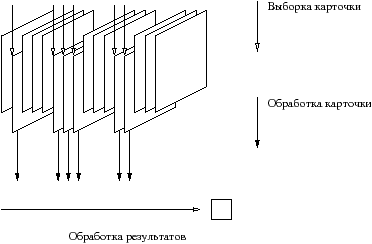
\includegraphics[width=\textwidth] {drafts/book009}}
	\caption{\label{fig:processing_a_request}Обработка запроса}
\end{figure}

В соответствии с этим, нам нужно 3 функции следующих типов:

\begin{itemize}
	\item \type{(data\_card -> bool) -> data\_card list -> data\_card list}
	
	\item \type{(data\_card -> 'a) -> data\_card list -> 'a list}
	
	\item \type{('a -> 'b -> 'b) -> 'a list -> 'b -> 'b}
\end{itemize}

Objective CAML предоставляет три функции высшего порядка, известные как 
итераторы, представленные на странице \ref{??}. Они соответствуют нашей 
спецификации.

\begin{lstlisting}[language=OCaml]
# List.find_all ;;
- : ('a -> bool) -> 'a list -> 'a list = <fun>
# List.map ;;
- : ('a -> 'b) -> 'a list -> 'b list = <fun>
# List.fold_right ;;
- : ('a -> 'b -> 'b) -> 'a list -> 'b -> 'b = <fun>
\end{lstlisting}

После того как мы определим функциональные аргументы, мы сможем воспользоваться 
этими функциями для реализации состояния в три этапа.

Для некоторых запросов нам понадобится следующая функция.

\begin{lstlisting}[language=OCaml]
# List.iter ;;
- : ('a -> unit) -> 'a list -> unit = <fun>
\end{lstlisting}

В случае, когда обработка данных ограничивается выводом на экран, вычислять 
нечего.

В следующих параграфах, мы увидим несколько простых методов обработки данных, а 
так же определение функций выражающих критерии выборки. Небольшой пример в 
заключении этой главы использует эти функции в соответствии с приведёнными выше 
принципами.

\subsection{Критерии выборки}
\label{subsec:selection_criteria}

В конкретном случае, логическая функция, которая определяет критерии выборки 
карточки, есть логическая комбинация свойств данных всех или части полей 
карточки. Каждое поле карточки, представленное строкой, может нести в себе 
информацию другого типа: целое число, число с плавающей запятой, и т.д..

\subsubsection{Критерии выборки по одному полю}

Выборка определённого поля по конкретному критерию будет осуществляется при 
помощи следующей функции \type{data\_base -> 'a -> string -> data\_card -> 
bool}. Параметр типом 'a соответствует типу информации хранимой в поле. Имя 
этого поля указанно аргументом с типом \type{string}.

\paragraph{Поля со строковым типом данных}

Определим два простых теста для работы с этим типом данных: тест на равенство с 
другой строкой и тест на \enq{не пустоту} строки.

\begin{lstlisting}[language=OCaml]
# let eq_sfield db s n dc =  (s = (field db n dc)) ;;
val eq_sfield : data_base -> string -> string -> data_card -> bool = <fun>
# let nonempty_sfield db n dc = ("" <> (field db n dc)) ;;
val nonempty_sfield : data_base -> string -> data_card -> bool = <fun>
\end{lstlisting}

\paragraph{Поля со типом данных число с плавающей запятой}

Для проверки информации содержащей числа с плавающей запятой достаточно 
перевести значение строки содержащей десятичное число в тип \type{float}. Вот 
несколько примеров полученных использованием настраиваемой функции 
\code{tst\_ffield}:

\begin{lstlisting}[language=OCaml]
# let tst_ffield r db v n dc = r v (float_of_string (field db n dc)) ;;
val tst_ffield :
  ('a -> float -> 'b) -> data_base -> 'a -> string -> data_card -> 'b = <fun>
# let eq_ffield = tst_ffield (=) ;;  
# let lt_ffield = tst_ffield (<) ;;  
# let le_ffield = tst_ffield (<=) ;; 
(* etc. *) 
\end{lstlisting}

Тип у данных функций:

\type{data\_base -> float -> string -> data\_card -> bool}.

Этот тип информации немного сложней, он зависит от представления даты в базе 
данных и требует определения способа сравнения дат.

Установим формат даты карточки как строку \code{дд.мм.гггг}. Для того чтобы 
получить дополнительные возможности сравнения, добавим в формат даты символ 
\code{'\_'}, заменяющий день, месяц или год. Даты сравниваются в 
лексикографическом порядке в формате \type{(год, месяц, день)}. Для того чтобы 
мы могли пользоваться выражениями как \enq{до июля 1998}, будем использовать 
сопоставление с образцом даты: \enq{\_.07.1998}. Сравнение даты с образцом 
реализуется функцией \code{tst\_dfield}, которая анализирует образец и создаёт 
{\it ad hoc} сравнивающую функцию. Для того чтобы определить эту универсальную 
функцию проверки даты, нам понадобятся несколько дополнительных функций.

Напишем две функции преобразующие дату (\code{ints\_of\_string}) и образцы даты 
(\code{ints\_of\_dpat}) в триплет целых чисел. Мы заменим символ \code{'\_'} 
образца на целое число 0.

\begin{lstlisting}[language=OCaml]
# let split_date = split '.' ;;
val split_date : string -> string list = <fun>
# let ints_of_string d =
   try  match split_date d with
           [j;m;a] -> [int_of_string a; int_of_string m; int_of_string j]
          |    _   -> failwith "Bad date format"
   with Failure("int_of_string") -> failwith "Bad date format" ;;
val ints_of_string : string -> int list = <fun>

# let ints_of_dpat d =
   let int_of_stringpat = function "_" -> 0 | s -> int_of_string s
   in try  match split_date d with
               [j;m;a] -> [ int_of_stringpat a; int_of_stringpat m; 
                            int_of_stringpat j ]
             | _ -> failwith "Bad date format"
      with Failure("int_of_string") -> failwith "Bad date pattern" ;;
val ints_of_dpat : string -> int list = <fun>
\end{lstlisting}

Напишем функцию теста, которая использует отношение целых \code{r}. Здесь мы 
реализуем лексикографический порядок, при этом мы обрабатываем специальный 
случай с нулём.

\begin{lstlisting}[language=OCaml]
# let rec app_dtst r d1 d2 = match d1, d2 with
    [] , [] -> false
  | (0::d1) , (_::d2) -> app_dtst r d1 d2
  | (n1::d1) , (n2::d2) -> (r n1 n2) || ((n1 = n2) && (app_dtst r d1 d2))
  | _, _ -> failwith "Bad date pattern or format" ;;
val app_dtst : (int -> int -> bool) -> int list -> int list -> bool = <fun>
\end{lstlisting}

Наконец, определим универсальную функцию \code{tst\_dfield} со следующими 
аргументами: отношение \code{r}, база данных \code{db}, образец \code{dp}, имя 
поля \code{nm} и карточка \code{dc}. Эта функция проверяет, что образец и 
извлечённое поле удовлетворяют отношение.

\begin{lstlisting}[language=OCaml]
# let tst_dfield r db dp nm dc = 
  r (ints_of_dpat dp) (ints_of_string (field db nm dc)) ;;
val tst_dfield :
  (int list -> int list -> 'a) ->
  data_base -> string -> string -> data_card -> 'a = <fun>
\end{lstlisting}

Теперь применим функцию к трём отношениям.

\begin{lstlisting}[language=OCaml]
# let eq_dfield = tst_dfield (=) ;;
# let le_dfield = tst_dfield (<=) ;;
# let ge_dfield = tst_dfield (>=) ;;
\end{lstlisting}

Тип этих функций следующий:

\type{data\_base -> string -> string -> data\_card -> bool}.

\subsubsection{Композиция критериев}

Три первые аргумента проверок, которые мы определили --- база данных, значение 
и имя поля. Когда мы пишем запросы базы данных, значения этих аргументов 
известны. Для базы \code{base\_ex} проверка \enq{до июля 1998} пишется 
следующим образом.

\begin{lstlisting}[language=OCaml]
# ge_dfield base_ex "_.07.1998" "Date" ;;
- : data_card -> bool = <fun>
\end{lstlisting}

Получается, что проверка это функция имеющая тип \type{data\_card -> bool}. 
Теперь нам нужно получить логические комбинации результатов подобных функций, 
применённых к одной и той же карточке. Для этого воспользуемся следующим 
итератором.

\begin{lstlisting}[language=OCaml]
# let fold_funs b c fs dc =
  List.fold_right (fun f -> fun r -> c (f dc) r) fs b ;;
val fold_funs : 'a -> ('b -> 'a -> 'a) -> ('c -> 'b) list -> 'c -> 'a = <fun>
\end{lstlisting}

Здесь \code{b} --- значение базы, функция \code{c} --- логический оператор, 
\code{fs} --- список функций проверки по полю и \code{dc} --- карточка.

В следующем примере получаем конъюнкцию (логическое произведение) и дизъюнкцию 
(логическая сумма) списка проверок.

\begin{lstlisting}[language=OCaml]
# let and_fold fs = fold_funs true (&) fs ;;
val and_fold : ('a -> bool) list -> 'a -> bool = <fun>
# let or_fold fs = fold_funs false (or) fs ;;
val or_fold : ('a -> bool) list -> 'a -> bool = <fun>
\end{lstlisting}

Для удобства определим отрицание функции проверки.

\begin{lstlisting}[language=OCaml]
# let not_fun f dc = not (f dc) ;;
val not_fun : ('a -> bool) -> 'a -> bool = <fun>
\end{lstlisting}

Для того, чтобы выбрать карточку, дата которой находится в определённом 
интервале, воспользуемся комбинаторными операторами.

\begin{lstlisting}[language=OCaml]
# let date_interval db d1 d2 = 
  and_fold [(le_dfield db d1 "Date"); (ge_dfield db d2 "Date")] ;;
val date_interval : data_base -> string -> string -> data_card -> bool =
  <fun>
\end{lstlisting}

\subsection{Обработка и вычисление}
\label{subsec:processing_and_computation}

Трудно представить себе все возможные обработки карточек или множество данных 
полученных после этой обработки. Тем не менее можно с уверенностью определить 
два класса таких обработок: численное вычисление и форматирование данных для 
печати. Рассмотрим каждый каждый случай на примере.

\subsubsection{Форматирование}

Подготовим к печати строку, содержащую имя члена ассоциации и кое-какую 
информацию.

Начнём с определения функции, которая из списка строк и разделителя создаёт 
строку состоящую из элемент списка разделённых сепаратором.

\begin{lstlisting}[language=OCaml]
# let format_list c = 
  let s = String.make 1 c in  
  List.fold_left (fun x y -> if x="" then y else x^s^y) "" ;;
val format_list : char -> string list -> string = <fun>
\end{lstlisting}

Определим функцию \code{extract}, которая создаёт список из полей с 
информацией, она извлекает из каждой карточки данные полей, имена которых 
переданы в списке.

\begin{lstlisting}[language=OCaml]
# let extract db ns dc = 
   List.map (fun n -> field db n dc) ns  ;;
val extract : data_base -> string list -> data_card -> string list = <fun>
\end{lstlisting}

Функция форматирования для печати выглядит следующим образом.

\begin{lstlisting}[language=OCaml]
# let format_line db ns dc =
  (String.uppercase (field db "Nom" dc))
  ^" "^(field db "Prenom" dc)
  ^"\t"^(format_list '\t' (extract db ns dc))
  ^"\n" ;;
val format_line : data_base -> string list -> data_card -> string = <fun>
\end{lstlisting}

Аргумент \code{ns} является списком с именами полей, которые нас интересуют. 
Поля разделены символом табуляции (\code{'\\t'}), а строка заканчивается 
возвратом каретки.

Вот как можно вывести на экран имена и фамилии членов ассоциации.

\begin{lstlisting}[language=OCaml]
# List.iter print_string (List.map (format_line base_ex []) base_ex.data) ;;
CHAILLOUX Emmanuel	
MANOURY Pascal	
PAGANO Bruno	
BARO Sylvain	
- : unit = ()
\end{lstlisting}

\subsubsection{Числовое вычисление}

Давайте вычислим сумму членских взносов для определённого множества карточек. 
Для этого достаточно извлечь нужное поле, привести к целому типу и вычислить 
сумму. Нужный результат может быть получен композицией этих функций. Для 
упрощения записи, определим инфиксный оператор композиции.

\begin{lstlisting}[language=OCaml]
# let (++) f g x = g (f x) ;;
val ++ : ('a -> 'b) -> ('b -> 'c) -> 'a -> 'c = <fun>
\end{lstlisting}

Воспользуемся этим оператором в следующем определении.

\begin{lstlisting}[language=OCaml]
# let total db dcs =
   List.fold_right ((field db "Montant") ++ float_of_string ++ (+.)) dcs 0.0 ;;
val total : data_base -> data_card list -> float = <fun>
\end{lstlisting}

Аналогичным образом можно применить эту функцию ко всей базе денных.

\begin{lstlisting}[language=OCaml]
# total base_ex base_ex.data ;;
- : float = 450
\end{lstlisting}

\subsection{Пример}
\label{subsec:an_example}

В заключении, проиллюстрируем на примере принципы, которые мы представили ранее 
в этой главе.

Рассмотрим два типа запроса базы данных:

\begin{itemize}
	\item запрос, возвращающий два списка, каждый из них содержит имя члена 
ассоциации, а так же электронный адрес для первого списка и почтовый адрес для 
второго, в зависимости от предпочтений.

	\item запрос, возвращающий состояние взносов на указанный период времени. 
Это  состояние будет хранить имена, фамилии, дату, взнос и сумму всех взносов.
\end{itemize}

\subsubsection{Списки адресов}

Для создания этих списков мы сначала выбираем в соответствии со значением поля 
\code{"Pref"} релевантные карточки, затем используем функцию 
\code{format\_line}.

\begin{lstlisting}[language=OCaml]
# let adresses_postales db =
  let dcs = List.find_all (eq_sfield db "adr" "Pref") db.data in
   List.map (format_line db ["Adresse"]) dcs ;;
val adresses_postales : data_base -> string list = <fun>

# let adresses_electroniques db =
  let dcs = List.find_all (eq_sfield db "mail" "Pref") db.data in
   List.map (format_line db ["Email"]) dcs ;;
val adresses_electroniques : data_base -> string list = <fun>
\end{lstlisting}

\subsubsection{Состояние взносов}

Вычисление состояния взносов выполняется по обычному принципы: выборка, затем 
обработка. В данном случае обработка состоит из двух частей: форматирование и 
вычисление общей суммы взносов.

\begin{lstlisting}[language=OCaml]
# let etat_cotisations db d1 d2 =
  let dcs = List.find_all (date_interval db d1 d2) db.data in
  let ls = List.map (format_line db ["Date";"Montant"]) dcs in
  let t = total db dcs in
   ls, t ;;
val etat_cotisations : data_base -> string -> string -> string list * float =
  <fun>
\end{lstlisting}

В результате этой функции мы получим пару состоящую из списка строк с 
информацией и суммы взносов.

\subsubsection{Основная программа}

Основная программа состоит из интерактивного цикла, выводящего результат 
запроса, который пользователь выбрал из меню. Здесь мы используем императивный 
стиль программирования, за исключением вывода результата при помощи итератора.

\begin{lstlisting}[language=OCaml]
# let main() =
  let db = read_base "association.dat" in
  let fin = ref false in
   while not !fin do
    print_string" 1: liste des adresses postales\n";
    print_string" 2: liste des adresses électroniques\n";
    print_string" 3: cotisations\n";
    print_string"  0 sortie\n";
    print_string"Votre choix : ";
    match read_int() with
      0 -> fin := true
    | 1 -> (List.iter print_string (adresses_postales db))
    | 2 -> (List.iter print_string (adresses_electroniques db))
    | 3
     -> (let d1 = print_string"Date de début : "; read_line() in
         let d2 = print_string"Date de fin : "; read_line() in
         let ls, t = etat_cotisations db d1 d2 in
          List.iter print_string ls;
          print_string"Total : "; print_float t; print_newline())
    | _ -> ()
   done;
   print_string"bye\n" ;;
val main : unit -> unit = <fun>
\end{lstlisting}

Мы вернёмся к этому примеру в главе \ref{??}, чтобы добавить к нему интерфейс 
при помощи web навигатора.

\subsection{Дополнительные возможности}
\label{subsec:further_work}

Вполне естественным будет добавить в базу данных нашего примера информацию о 
типе каждого поля. Эта информация пригодится в случае если мы хотим определить 
универсальные (generic) операторы сравнения со следующим типом \type{data\_base 
-> 'a -> string -> data\_card -> bool}. Имя поля (третий аргумент) позволяет 
передавать управление соответствующей функции сравнения и проверки. 

\section{Интерпретатор языка BASIC}
\label{sec:basic_interpreter}

В данном разделе мы рассмотрим интерпретатор языка Basic. Это программа, которая 
выполняет другие программы написанные на языке Basic. Конечно, мы ограничимся 
лишь частью команд этого языка, наш интерпретатор будет распознавать следующие 
команды:

\begin{description}
	\item[PRINT] {\it выражение}

	Выводит результат вычисления выражения.

	\item[INPUT] {\it переменная}

	Выводит {\it приглашение} на экран (?), ожидает ввод целого числа с 
клавиатуры и затем присваивает это число переменной.

	\item[LET] {\it переменная = выражение}

	Присваивает переменной результат вычисления выражения.

	\item[GOTO] {\it номер строки}

	Выполнение продолжится с указанной строки.

	\item[IF] {\it условие} {\bf THEN} {\it номер строки}

	Выполнение продолжится с указанной строки если условие верно.
	
	\item[REM] {\it строка символов}

	Комментарии.
\end{description}

Каждая строка программы Basic помечена номером и содержит лишь одну инструкцию. 
Программа, вычисляющая факториал для числа введённого с клавиатуры, выглядит 
следующим образом:

\begin{lstlisting}[language={[Visual]Basic}]
 5  REM inputting the argument
10  PRINT " factorial of:"
20  INPUT A
30  LET B = 1 
35  REM beginning of the loop
40  IF A <= 1 THEN 80 
50  LET B = B * A
60  LET A = A - 1
70  GOTO 40 
75  REM prints the result
80  PRINT B
\end{lstlisting}

Реализуем также мини–редактор по принципу интерактивного цикла. У нас должна 
быть возможность добавлять новые строки, вывод программы и её вычисление. 
Запуск предыдущей программы осуществляется командой \code{RUN}. Пример 
вычисления этой программы.

\begin{lstlisting}
> RUN
 factorial of: ? 5
120
\end{lstlisting}

Это вычисление можно разбить на несколько разных этапов.

\begin{description}
	\item[Описание абстрактного синтаксиса]

	необходимо определить типы данных для описания программ на Basic, а так же 
другие компоненты (строки, комментарии, выражения, и т.д.)

	\item[Вывод программы]

	эта часть состоит в переводе программы на Basic из внутреннего формата в 
строки, для того чтобы вывести ее на экран.

	\item[Лексический и синтаксический анализ]

	обе эти части проделывают обратную операцию, то есть перевод строки во 
внутренний формат программы на Basic (абстрактный синтаксис)

	\item[Вычисление]

	это основа интерпретатора. Далее мы увидим что функциональный язык как 
Objective CAML особенно хорошо подходит для решения подобных проблем.

	\item[Интерактивный цикл]

	здесь реализуется все вышесказанное.
\end{description}

\subsection{Абстрактный синтаксис}
\label{subsec:abstract_syntax}

% TODO переделать по-нормальному
\begin{verbatim}
Unary_Op        ::=     -    |    !
Binary_Op       ::=     +    |    -    |    *    |    /    |    %
        |       =    |    <    |    >    |    <=    |    >=    |    <>
        |       &    |    ' | '
Expression      ::=     integer
        |       variable
        |       "string"
        |       Unary_Op   Expression
        |       Expression   Binary_Op   Expression
        |       ( Expression )
Command         ::=     REM string
        |       GOTO integer
        |       LET variable = Expression
        |       PRINT Expression
        |       INPUT variable
        |       IF Expression THEN integer
 
Line    ::=     integer Command
 
Program         ::=     Line
        |       Line Program
 
Phrase  ::=     Line | RUN | LIST | END
\end{verbatim}

Заметим, что правильность выражения с точки зрения грамматики не означает 
возможность его вычисления. Например, \code{1 + ``hello''} есть выражение, 
однако его невозможно вычислить. Это сделано с целью облегчить абстрактный 
синтаксис языка Basic. Расплата за это --- программы на Basic, синтаксически 
правильные, могут привести к ошибке из--за несоответствия типов.

Теперь определить типы данных Objective CAML просто, достаточно перевести 
абстрактный синтаксис в тип сумма.

\begin{lstlisting}[language=OCaml]
# type op_unr = OPPOSE | NON  ;;
# type op_bin = PLUS | MOINS | MULT | DIV | MOD  
             | EGAL | INF | INFEQ | SUP | SUPEQ | DIFF 
             | ET | OU  ;;
# type expression = 
     ExpInt of int 
   | ExpVar of string
   | ExpStr of string 
   | ExpUnr of op_unr * expression
   | ExpBin of expression * op_bin * expression  ;;
# type instruction = 
     Rem of string
   | Goto of int 
   | Print of expression
   | Input of string 
   | If of expression * int 
   | Let of string * expression  ;;
# type ligne = { num : int ; inst : instruction }  ;;
# type program = ligne list  ;;
\end{lstlisting}

Определим синтаксис команд для мини--редактора.

\begin{lstlisting}[language=OCaml]
# type phrase =  Ligne of ligne | List | Run | End  ;;
\end{lstlisting}

Обычно, чтобы облегчить синтаксис, программистам разрешается не указывать все 
скобки. Например, под выражением $1 + 3 * 4$ подразумевается $1 + (3 * 4)$. 
Для этого, каждому оператору языка присваивается целое число --- приоритет:

\begin{lstlisting}[language=OCaml]
# let priority_ou = function NON -> 1 | OPPOSE -> 7
 let priority_ob = function 
     MULT | DIV  -> 6
   | PLUS | MOINS -> 5
   | MOD -> 4
   | EGAL | INF | INFEQ | SUP | SUPEQ | DIFF -> 3
   | ET | OU -> 2 ;;
val priority_ou : op_unr -> int = <fun>
val priority_ob : op_bin -> int = <fun>
\end{lstlisting}

Целые числа означают, так называемый, приоритет операторов. Далее мы увидим как 
они используются при синтаксическом анализе или выводе программ на экран.

\subsection{Вывод программы на экран}
\label{subsec:program_pretty_printing}

Для того, чтобы вывести программу хранящуюся в памяти, необходимо уметь 
перевести строку программы из абстрактного синтаксиса в строку символов.

Перевод операторов может быть получен легко и просто:

\begin{lstlisting}[language=OCaml]
# let pp_opbin = function  
     PLUS -> "+" | MULT -> "*" | MOD   -> "%" | MOINS -> "-" 
   | DIV -> "/"  | EGAL -> " = " | INF -> " < " 
   | INFEQ -> " <= "   | SUP   -> " > " 
   | SUPEQ -> " >= "   | DIFF  -> " <> " | ET -> " & " | OU -> " | "  
 let pp_opunr = function OPPOSE -> "-"  | NON -> "!"  ;;
val pp_opbin : op_bin -> string = <fun>
val pp_opunr : op_unr -> string = <fun>
\end{lstlisting}

Вывод выражений соблюдает приоритет операторов для того чтобы получить выражение 
с минимумом скобок. Мы используем скобки лишь в случае если оператор в 
под--выражении справа от оператора менее приоритетный всего оператор целого 
выражения. К тому же, арифметические операторы ассоциативные слева, это значит 
что выражение $1 - 2 - 3$ эквивалентно $(1 - 2) - 3$.

Чтобы получить данный результат, создадим две функции \code{ppl} и \code{ppr}, 
которые будут обрабатывать левые и правые под--деревья соответственно. У этих 
функций два аргумента: дерево выражений и приоритет оператора в корне дерева, 
основываясь на значении последнего мы решим нужны--ли скобки в выражении или 
нет. Чтобы учитывать ассоциативность операторов мы различаем левое под--дерево 
от правого. Если приоритет текущего оператора одинаков с корневым, то ставить 
скобки для левого под--дерева не нужно. Для правого под--дерева скобки могут 
понадобиться, как в следующих случаях: $1 - (2 - 3)$ или $1 - (2 + 3)$.

Начальное дерево рассматривается как левое под--дерево оператора с минимальным 
приоритетом $(0)$. Вот как работает функция вывода выражений 
\code{pp\_expression}:

\begin{lstlisting}[language=OCaml]
# let parenthese x = "(" ^ x ^ ")";;  
val parenthese : string -> string = <fun>
# let pp_expression = 
  let rec ppg pr = function 
       ExpInt n -> (string_of_int n)
     | ExpVar v -> v 
     | ExpStr s -> "\"" ^ s ^ "\"" 
     | ExpUnr (op,e) -> 
         let res = (pp_opunr op)^(ppg (priority_ou op) e) 
         in if pr=0 then res else parenthese res 
     | ExpBin (e1,op,e2) -> 
         let pr2 = priority_ob op
         in let res = (ppg pr2 e1)^(pp_opbin op)^(ppd pr2 e2)
         (* parenthèse si la priorité n'est pas supérieure *)
         in if pr2 >= pr then res else parenthese res
   and ppd pr exp = match exp with 
     (*  les sous-arbres droits ne diffèrent  *)
     (*  que pour les opérateurs binaires     *) 
       ExpBin (e1,op,e2) -> 
         let pr2 = priority_ob op
         in let res = (ppg pr2 e1)^(pp_opbin op)^(ppd pr2 e2)
         in if pr2 > pr then res else parenthese res
     | _ -> ppg pr exp
   in ppg 0 ;;
val pp_expression : expression -> string = <fun>
\end{lstlisting}

Для вывода инструкций, воспользуемся предыдущей функцией. При этом добавим номер 
перед каждой инструкцией.

\begin{lstlisting}[language=OCaml]
# let pp_instruction = function 
     Rem s     ->  "REM " ^ s
   | Goto n    ->  "GOTO " ^ (string_of_int n)
   | Print e   ->  "PRINT " ^ (pp_expression e)
   | Input v   ->  "INPUT " ^ v
   | If (e,n)  ->  "IF "^(pp_expression e)^" THEN "^(string_of_int n)
   | Let (v,e) ->  "LET " ^ v ^ " = " ^ (pp_expression e)  ;;
val pp_instruction : instruction -> string = <fun>
# let pp_ligne l = (string_of_int l.num) ^ "  " ^ (pp_instruction l.inst)  ;;
val pp_ligne : ligne -> string = <fun>
\end{lstlisting}

\subsection{Лексический анализ}
\label{subsec:Lexing}

Синтаксический и лексический анализ реализуют противоположную выводу на экран 
операцию. Для полученной строки создаётся синтаксическое дерево. Лексический 
анализ разбивает строку инструкции на независимые лексические части, называемые 
лексемами. Для этого добавим следующий тип в Objective CAML:

\begin{lstlisting}[language=OCaml]
# type lexeme = Lint of int 
             | Lident of string 
             | Lsymbol of string  
             | Lstring of string
             | Lfin ;;
\end{lstlisting}

Для обозначения конца выражения мы добавили специальную лексему \code{Lend}. 
Она не является частью анализируемой строки, а добавляется функцией 
лексического анализа (см. \ref{subsec:parsing}).

Для анализа строки мы используем тип запись содержащую изменяемое поле, значение 
которого указывает на часть строки, которую осталось обработать. Размер строки 
будет необходим во многих случаях, поэтому мы храним это константное значение в 
записи.

\begin{lstlisting}[language=OCaml]
# type chaine_lexer = {chaine:string; mutable courant:int; taille:int } ;;
\end{lstlisting}

Такой способ определения лексического анализа можно рассматривать как применение 
функции к значению с типом \type{string\_lexer}, в результате чего получим 
значение типа \type{lexeme}. Изменение индекса строки, которую осталось 
проанализировать, получается в результате побочного эффекта.

\begin{lstlisting}[language=OCaml]
# let init_lex s = { chaine=s; courant=0 ; taille=String.length s } ;;
val init_lex : string -> chaine_lexer = <fun>
# let avance cl = cl.courant <- cl.courant+1  ;;
val avance : chaine_lexer -> unit = <fun>
# let avance_n cl n = cl.courant <- cl.courant+n ;;
val avance_n : chaine_lexer -> int -> unit = <fun>
# let extrait pred cl = 
   let st = cl.chaine and ct = cl.courant in
   let rec ext n = if n<cl.taille && (pred st.[n]) then ext (n+1) else n in 
   let res = ext ct 
   in cl.courant <- res ; String.sub cl.chaine ct (res-ct)  ;;
val extrait : (char -> bool) -> chaine_lexer -> string = <fun>
\end{lstlisting}

Следующие функции извлекают лексему из строки и изменяют маркер текущей позиции. 
Функции \code{extract\_int} и \code{extract\_ident} извлекают целое число и 
идентификатор соответственно.

\begin{lstlisting}[language=OCaml]
# let extrait_int = 
    let est_entier = function '0'..'9' -> true | _ -> false  
    in function cl -> int_of_string (extrait est_entier cl)
 let extrait_ident =
    let est_alpha_num = function 
      'a'..'z' | 'A'..'Z' | '0' .. '9' | '_' -> true 
    | _ -> false  
    in extrait est_alpha_num ;;
val extrait_int : chaine_lexer -> int = <fun>
val extrait_ident : chaine_lexer -> string = <fun>
\end{lstlisting}

Функция \code{lexer} использует обе предыдущие функции для извлечения лексем.

\begin{lstlisting}[language=OCaml]
# exception LexerErreur ;;
exception LexerErreur
# let  rec lexer cl = 
   let lexer_char c = match c with 
       ' ' 
     | '\t'     -> avance cl ; lexer cl 
     | 'a'..'z' 
     | 'A'..'Z' -> Lident (extrait_ident cl)
     | '0'..'9' -> Lint (extrait_int cl)
     | '"'      -> avance cl ; 
                   let res = Lstring (extrait ((<>) '"') cl) 
                   in avance cl ; res 
     | '+' | '-' | '*' | '/' | '%' | '&' | '|' | '!' | '=' | '(' | ')'  -> 
                   avance cl; Lsymbol (String.make 1 c)
     | '<' 
     | '>'      -> avance cl; 
                   if cl.courant >= cl.taille then Lsymbol (String.make 1 c)
                   else  let cs = cl.chaine.[cl.courant] 
                         in ( match (c,cs) with 
                                ('<','=') -> avance cl; Lsymbol "<=" 
                                    | ('>','=') -> avance cl; Lsymbol ">="
                              | ('<','>') -> avance cl; Lsymbol "<>"
                              |     _     -> Lsymbol (String.make 1 c) )
     | _ -> raise LexerErreur
   in 
      if cl.courant >= cl.taille then Lfin 
      else lexer_char cl.chaine.[cl.courant] ;;
val lexer : chaine_lexer -> lexeme = <fun>
\end{lstlisting}

Принцип действия функции \code{lexer} очень простой: здесь анализируется 
текущий символ строки, в зависимости от его значения возвращается 
соответствующая лексема и текущая позиция перемещается на начало следующей 
лексемы. Это очень простой и эффективный подход, две лексемы могут различаться 
по первому же символу. Для символа \code{`<'} необходимо проверить следующий 
символ, за ним может следовать \code{`='} или \code{`>'} и является другой 
лексемой. То же самое касается символа \code{`>'}.

\subsection{Синтаксический анализ}
\label{subsec:parsing}

При анализе выражений языка возникают некоторые проблемы; знание начала 
выражения не достаточно для того, чтобы определить всю его структуру. Пусть мы 
анализируем часть строки $1 + 2 + 3$. В зависимости от того, что за этим 
следует $+ 4$ или $* 4$, полученные деревья для части $1 + 2 + 3$ различаются 
(см. рис. \ref{fig:basic_abstract_syntax_tree_examples}).

\begin{figure}[h]
	\center{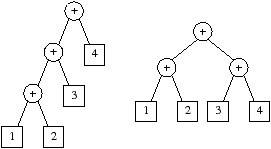
\includegraphics {drafts/book010}}
	\caption{\label{fig:basic_abstract_syntax_tree_examples}Абстрактные 
синтаксические деревья}
\end{figure}

Однако, структура дерева для $1 + 2$ одинакова в обоих случаях, поэтому мы 
можем его построить. В связи с тем что у нас отсутствует информация о части 
$+ 3$, мы временно сохраним это информацию до нужного момента.

При построении дабстрактного синтаксического дерева мы воспользуемся стековым 
автоматом, схожий с тем, который используется {\it yacc} (см. \ref{??}). 
Лексему читаются одна за другой и помещаются в стек до тех пор, пока у нас не 
будет достаточно информации, чтобы построить выражение. После этого, лексемы 
удаляются из стека и заменяются построенным выражением. Эта операция называется 
редукцией. 

Тип помещаемых в стек элементов следующий:

\begin{lstlisting}[language=OCaml]
# type exp_elem = 
     Texp of expression   (* expression         *)
   | Tbin of op_bin       (* opérateur binaire  *)
   | Tunr of op_unr       (* opérateur unaire   *)
   | Tpg                  (* parenthèse gauche  *) ;;
\end{lstlisting}

Заметим, что правые скобки не сохраняются, так как лишь левые скобки важны при 
операции редукции.

На рисунке \ref{fig:basic_abstract_syntax_tree_construction_example} 
проиллюстрировано изменение стека при анализе выражения $(1 + 2 * 3) * 4$. 
Символ над стрелкой есть текущий символ строки.

\begin{figure}[h]
	\center{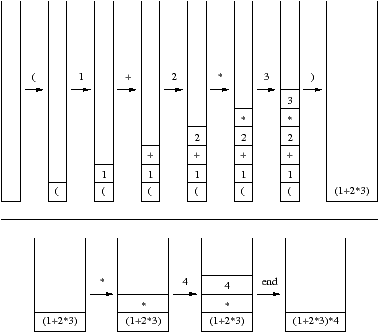
\includegraphics {drafts/book011}}
	\caption{\label{fig:basic_abstract_syntax_tree_construction_example}Basic: 
Пример создания абстрактного синтаксического дерева}
\end{figure}

Определим исключение для синтаксических ошибок.

\begin{lstlisting}[language=OCaml]
# exception ParseError ;;
\end{lstlisting}

Сначала определим операторы при помощи символов.

\begin{lstlisting}[language=OCaml]
# let symb_unr = function 
   "!" -> NON | "-" -> OPPOSE | _ -> raise ParseErreur 
 let symb_bin = function
     "+" -> PLUS | "-" -> MOINS | "*" -> MULT | "/" -> DIV | "%" -> MOD 
   | "=" -> EGAL | "<" -> INF | "<=" -> INFEQ | ">" -> SUP 
   | ">=" -> SUPEQ | "<>" -> DIFF | "&" -> ET | "|" -> OU 
   | _ -> raise ParseErreur 
 let tsymb s = try Tbin (symb_bin s) with ParseErreur -> Tunr (symb_unr s) ;;
val symb_unr : string -> op_unr = <fun>
val symb_bin : string -> op_bin = <fun>
val tsymb : string -> exp_elem = <fun>
\end{lstlisting}

Функция \code{reduce} реализует редукцию стека. Существует два случая, в 
которых стек начинается:

\begin{itemize}
	\item выражение, с последующим унарным оператором

	\item выражение, затем бинарный оператор и другое выражение. 
\end{itemize}

Кроме того, другой аргумент функции \code{reduce} --- это минимальный 
приоритет, который должен иметь оператор, чтобы редукция имела место. Для 
приведения без условий достаточно указать минимальный нулевой приоритет.

\begin{lstlisting}[language=OCaml]
# let reduce pr = function 
     (Texp e)::(Tunr op)::st  when  (priority_uop op) >= pr
        -> (Texp (ExpUnr (op,e)))::st
   | (Texp e1)::(Tbin op)::(Texp e2)::st  when  (priority_binop op) >= pr
        -> (Texp (ExpBin (e2,op,e1)))::st 
   | _ -> raise ParseError ;;
val reduce : int -> exp_elem list -> exp_elem list = <fun>
\end{lstlisting}

Заметим, что элементы выражения помещаются в стек в порядке чтения, из--за чего 
необходимо поменять местами операнды бинарной операции.

\code{stack\_or\_reduce} это главная функция синтаксического анализа, в 
соответствии с переданной ей лексемой она либо помещает новый элемент в стек 
либо выполняет редукцию.

\begin{lstlisting}[language=OCaml]
# let rec stack_or_reduce lex stack = match lex , stack with 
     Lint n ,  _      ->  (Texp (ExpInt n))::stack 
   | Lident v ,  _    ->  (Texp (ExpVar v))::stack 
   | Lstring s , _    ->  (Texp (ExpStr s))::stack
   | Lsymbol "(" , _  ->  Tlp::stack
   | Lsymbol ")" , (Texp e)::Tlp::st  ->  (Texp e)::st
   | Lsymbol ")" , _ -> stack_or_reduce lex (reduce 0 stack) 
   | Lsymbol s , _ 
        -> let symbol = 
             if s<>"-" then tsymb s 
             (* remove the ambiguity of the ``-'' symbol           *)
             (* according to the last exp element put on the stack *)
             else match stack 
                  with (Texp _)::_  ->  Tbin MINUS 
                                | _ ->  Tunr UMINUS 
           in ( match symbol with 
                  Tunr op  ->  (Tunr op)::stack 
                | Tbin op  -> 
                    ( try stack_or_reduce lex (reduce (priority_binop op) 
                                               stack )
                      with ParseError -> (Tbin op)::stack )
                | _ -> raise ParseError )
   | _ , _ -> raise ParseError ;;
val stack_or_reduce : lexeme -> exp_elem list -> exp_elem list = <fun>
\end{lstlisting}

После того как все лексемы извлечены и помещены в стек, дерево абстрактного 
синтаксиса может быть построено из элементов оставшихся в стеке --- это задача 
функции \code{reduce\_all}. Если анализируемое выражение было правильно 
сформировано, то в стеке должен остаться лишь один элемент, содержащий дерево 
этого выражения.

\begin{lstlisting}[language=OCaml]
# let rec reduce_all = function
   | [] -> raise ParseError
   | [Texp x] -> x 
   | st -> reduce_all (reduce 0 st) ;;
val reduce_all : exp_elem list -> expression = <fun>
\end{lstlisting}

Основной функцией анализа выражений является \code{parse\_exp}. Она 
просматривает строку, извлекает различные лексемы и передаёт их функции 
\code{stack\_or\_reduce}. Анализ прекращается, когда текущая лексема 
соответствует предикату переданному в аргументе.

\begin{lstlisting}[language=OCaml]
# let parse_exp stop cl = 
   let p = ref 0 in 
   let rec parse_one stack  = 
     let l = ( p:=cl.current ; lexer cl)
     in if not (stop l) then parse_one (stack_or_reduce l stack)
        else ( cl.current <- !p ; reduce_all stack )
   in parse_one []  ;;
val parse_exp : (lexeme -> bool) -> string_lexer -> expression = <fun>
\end{lstlisting}

Заметим, что лексема, которая определяет конец анализа, не используется при 
построении выражения. Для того чтобы проанализировать эту лексему позднее, 
необходимо установить текущую позицию на её начало (переменная \code{p}).

Перейдём теперь к анализу строки с инструкцией.

\begin{lstlisting}[language=OCaml]
# let parse_cmd cl = match lexer cl with 
     Lident s -> ( match s with 
         "REM" -> Rem (extract (fun _ -> true) cl)
       | "GOTO" -> Goto (match lexer cl with 
                           Lint p -> p 
                         | _ -> raise ParseError)
       | "INPUT" -> Input (match lexer cl with 
                             Lident v -> v 
                           | _ -> raise ParseError)
       | "PRINT" -> Print (parse_exp ((=) Lend) cl)
       | "LET" -> 
           let l2 = lexer cl and l3 = lexer cl 
           in ( match l2 ,l3 with 
                    (Lident v,Lsymbol "=") -> Let (v,parse_exp ((=) Lend) cl)
                  | _ -> raise ParseError )
       | "IF" -> 
           let test = parse_exp ((=) (Lident "THEN")) cl 
           in ( match ignore (lexer cl) ; lexer cl with 
                   Lint n  ->  If (test,n) 
                 | _ -> raise ParseError )
       | _ -> raise ParseError ) 
   | _ -> raise ParseError  ;;
val parse_cmd : string_lexer -> command = <fun>
\end{lstlisting}

И наконец, главная функция синтаксического анализа команд введённых 
пользователем в интерактивном цикле.

\begin{lstlisting}[language=OCaml]
# let parse str = 
   let cl = init_lex str 
   in match lexer cl with 
       Lint n -> Line { num=n ; cmd=parse_cmd cl }
     | Lident "LIST" -> List 
     | Lident "RUN" -> Run 
     | Lident "END" -> PEnd 
     | _ -> raise ParseError  ;;
val parse : string -> phrase = <fun>
\end{lstlisting}

\subsection{Вычисление}
\label{subsec:evaluation}

Программа на Basic состоит из набора строк и выполнение начинается с первой 
строки. Интерпретация строки программы заключается в исполнении задачи 
инструкции, которая находится на этой строке. Существует три множества 
инструкций: ввод/вывод ({\bf PRINT} и {\bf INPUT}), декларация переменных или 
присвоение ({\bf LET}) и переход ({\bf GOTO} и {\bf THEN}). Инструкции 
ввода/вывода реализуют взаимодействие с пользователем, для этого будут 
использованы соответствующие команды Objective CAML.

Для объявления и присвоения переменных, необходимо уметь вычислить значение 
арифметического выражение и знать расположение в памяти этой переменной. 
Результат вычисление выражения может быть либо целым числом, либо булевым 
значением, либо строкой. Сгруппируем их в типе \type{value}.

\begin{lstlisting}[language=OCaml]
# type value = Vint of int | Vstr of string | Vbool of bool  ;;
\end{lstlisting}

При объявлении переменной, нужно выделить память, чтобы хранить значение 
ассоциированное этой переменной. Для изменении переменной необходимо поменять 
значение связанно с именем переменной. Соответственно, программа Basic 
использует окружение, которое хранит связки имя переменной---значение. Данное 
окружение представлено в виде списка из пар (имя, значение).

\begin{lstlisting}[language=OCaml]
# type environment = (string * value) list ;;
\end{lstlisting}

Для того чтобы получить содержимое переменной мы используем её имя. При 
изменении значения переменной, меняется соответствующая пара.

В инструкциях перехода, условного или безусловного, указывается номер строки на 
которой должно продолжится выполнение программы. По умолчанию --- это следующая 
строка. В связи с этим, необходимо запомнить номер текущей строки.

Список инструкций из которых состоит программа, редактируемая в интерактивном 
цикле, не подходит для эффективного выполнения программы. Действительно, для 
того чтобы реализовать переход (\code{If} и \code{Goto}) необходимо 
пересмотреть весь список инструкций, чтобы найти строку с нужным номером. Для 
того чтобы можно было напрямую перейти на нужную строку, достаточно заменить 
структуру списка на вектор. В данном случае при переходе будет использоваться не 
номер строки, а её индекс в векторе. В этом случае, перед запуском программы 
командой \code{RUN}, проделаем пре--обработку инструкций, называемую 
компоновкой (assembly). По некоторым причинам, которые будут объяснены в 
следующем параграфе, скомпонованная программа представлена вектором строк, а не 
инструкций.

\begin{lstlisting}[language=OCaml]
# type code = line array ;;
\end{lstlisting}

Как и для калькулятора из прошлых глав, вычислитель использует состояние, 
которое изменяется при каждом вычислении. Информация, которую необходимо знать в 
каждый момент --- это программа в целом, следующая строка на выполнение и 
значения переменных. Выполняемая программа отличается от программы набранной в 
интерактивном цикле. Вместо того списка инструкций, мы используем вектор 
инструкций. Таким образом состояние программы описывается следующим типом.

\begin{lstlisting}[language=OCaml]
# type state_exec = { line:int ; xprog:code ; xenv:environment } ;;
\end{lstlisting}

Ошибки могут возникнуть в двух следующих случаях: вычисление выражения и переход 
на несуществующую строку. Соответственно, нужно обработать эти оба случая, чтобы 
интерпретатор корректно останавливался и выводил сообщение об ошибке. Определим 
исключение, а также функцию, которая будет его возбуждать и указывать номер 
строки на которой оно произошло.

\begin{lstlisting}[language=OCaml]
# exception RunError of int 
 let runerr n = raise (RunError n) ;;
exception RunError of int
val runerr : int -> 'a = <fun>
\end{lstlisting}

\subsection{Компоновка}
\label{subsubsec:assembly}

Компоновка программы, состоящей из списка нумерованных строк (тип 
\type{program}), заключается в переводе списка в вектор и корректировки 
инструкций перехода. Эта корректировка реализуется связкой номера строки и 
соответствующего ей индекса вектора. Для облегчения задачи, мы создаём вектор 
нумерованных строки. Данный вектор будет просматриваться каждый раз, когда 
необходимо найти индекс связанный со строкой. Если номер строки не найден, будет 
возвращено значение -1.

\begin{lstlisting}[language=OCaml]
# exception Result_lookup_index of int ;;
exception Result_lookup_index of int
# let lookup_index tprog num_line =
   try 
     for i=0 to (Array.length tprog)-1 do 
       let num_i = tprog.(i).num
       in if num_i=num_line then raise (Result_lookup_index i)
          else if num_i>num_line then raise (Result_lookup_index (-1))
     done ;
     (-1 )
   with Result_lookup_index i -> i ;;
val lookup_index : line array -> int -> int = <fun>

# let assemble prog =
   let tprog = Array.of_list prog in
     for i=0 to (Array.length tprog)-1 do
       match tprog.(i).cmd with
           Goto n -> let index = lookup_index tprog n
                     in tprog.(i) <- { tprog.(i) with cmd = Goto index }
         | If(c,n) -> let index = lookup_index tprog n
                      in tprog.(i) <- { tprog.(i) with cmd = If (c,index) }
         | _ -> ()
     done ;
   tprog ;;
val assemble : line list -> line array = <fun>
\end{lstlisting}

\subsection{Вычисление выражений}
\label{subsubsec:expression_evaluation}

Функция вычисления выражений обходит дерево абстрактного синтаксиса и выполняет 
операции, указанные в каждом узле дерева.

В следующих случаях возбуждается исключение \code{RunError}: несоответствие 
типов, деление на ноль и необъявленная переменная.

\begin{lstlisting}[language=OCaml]
# let rec eval_exp n envt expr = match expr with 
     ExpInt p  ->  Vint p
   | ExpVar v  -> ( try List.assoc v envt with Not_found -> runerr n )
   | ExpUnr (UMINUS,e) ->  
       ( match eval_exp n envt e with 
           Vint p -> Vint (-p) 
         | _ -> runerr n )
   | ExpUnr (NOT,e) ->  
       ( match eval_exp n envt e with 
           Vbool p -> Vbool (not p) 
         | _ -> runerr n )
   | ExpStr s -> Vstr s  
   | ExpBin (e1,op,e2) 
       -> match eval_exp n envt e1 , op , eval_exp n envt e2 with
               Vint v1 , PLUS   , Vint v2  ->  Vint (v1 + v2) 
             | Vint v1 , MINUS  , Vint v2  ->  Vint (v1 - v2) 
             | Vint v1 , MULT   , Vint v2  ->  Vint (v1 * v2) 
             | Vint v1 ,  DIV   , Vint v2  when v2<>0 ->  Vint (v1 / v2) 
             | Vint v1 ,  MOD   , Vint v2  when v2<>0 ->  Vint (v1 mod v2) 
 
             | Vint v1 , EQUAL   , Vint v2  ->  Vbool (v1 = v2) 
             | Vint v1 , DIFF    , Vint v2  ->  Vbool (v1 <> v2) 
             | Vint v1 ,  LESS   , Vint v2  ->  Vbool (v1 < v2) 
             | Vint v1 ,  GREAT  , Vint v2  ->  Vbool (v1 > v2) 
             | Vint v1 , LESSEQ  , Vint v2  ->  Vbool (v1 <= v2) 
             | Vint v1 , GREATEQ , Vint v2  ->  Vbool (v1 >= v2) 
 
             | Vbool v1 , AND , Vbool v2  ->  Vbool (v1 && v2) 
             | Vbool v1 , OR , Vbool v2  ->  Vbool (v1 || v2) 
 
             | Vstr v1 , PLUS , Vstr v2 -> Vstr (v1 ^ v2) 
             | _ , _ , _  -> runerr n  ;;
val eval_exp : int -> (string * value) list -> expression -> value = 
<fun>
\end{lstlisting}

\subsection{Вычисление инструкций}
\label{subsubsec:command_evaluation}

Для того, чтобы реализовать вычисление строки инструкций, нам понадобятся 
несколько дополнительных функций.

Добавление новой связки (имя переменной--значение) в окружение, заменяет 
старую, с таким же именем, если она существует.

\begin{lstlisting}[language=OCaml]
# let rec add v e env = match env with 
     [] -> [v,e]
   | (w,f)::l -> if w=v then (v,e)::l else (w,f)::(add v e l) ;;
val add : 'a -> 'b -> ('a * 'b) list -> ('a * 'b) list = <fun>
\end{lstlisting}

Другая функция, для вывода целых чисел или строк, пригодится при вычислении 
команды \code{PRINT}.

\begin{lstlisting}[language=OCaml]
# let print_value v = match v with 
     Vint n -> print_int n
   | Vbool true -> print_string "true"
   | Vbool false -> print_string "false"
   | Vstr s -> print_string s ;;
val print_value : value -> unit = <fun>
\end{lstlisting}

Вычисление инструкции есть переход из одного состояния в другое. В частности, 
окружение будет изменено, если инструкция это присвоение. Значение следующей 
строки на выполнение изменяется каждый раз. Если строка не существует, вернём 
значение -1.

\begin{lstlisting}[language=OCaml]
# let next_line state =
  let n = state.line+1 in
   if n < Array.length state.xprog then n else -1 ;;
val next_line : state_exec -> int = <fun>
# let eval_cmd state =
   match state.xprog.(state.line).cmd with 
     Rem _    ->  { state with line = next_line state }
   | Print e  ->  print_value (eval_exp state.line state.xenv e) ; 
                  print_newline () ;
                  { state with line = next_line state }
   | Let(v,e) ->  let ev = eval_exp state.line state.xenv e 
                    in { state with line = next_line state ; 
                                   xenv = add v ev state.xenv }
   | Goto n   ->  { state with line = n }
   | Input v  ->  let x = try read_int () 
                          with Failure "int_of_string" -> 0
                  in { state with line = next_line state; 
                                 xenv = add v (Vint x) state.xenv }
   | If (t,n) ->  match eval_exp state.line state.xenv t with 
                    Vbool true  -> { state with line = n }
                  | Vbool false -> { state with line = next_line state }
                  | _ -> runerr state.line  ;;
val eval_cmd : state_exec -> state_exec = <fun>
\end{lstlisting}

При каждом вызове функция перехода из одного состояние в другое 
\code{eval\_cmd} ищет текущую строку, выполняет её и затем устанавливает номер 
следующей строки как текущую строку. Если мы достигли последней строки 
программы, то номеру текущей строки присваивается значение -1, что позволит нам 
остановить программу.

\subsection{Вычисление программы}
\label{subsubsec:program_evaluation}

Будет рекурсивно применять функцию перехода, до тех пор, пока не получим 
состояние, в котором номер текущей строки равен -1.

\begin{lstlisting}[language=OCaml]
# let rec run state = 
  if state.line = -1 then state else run (eval_cmd state) ;;
val run : state_exec -> state_exec = <fun>
\end{lstlisting}

\subsection{Последние штрихи}
\label{subsec:finishing_touches}

Осталось лишь реализовать мини–редактор и собрать воедино все части программы, 
реализованные ранее.

Функция \code{insert} вставляет новую строку в соответствующее место в 
программе.

\begin{lstlisting}[language=OCaml]
# let rec insert line p = match p with  
     [] -> [line]
   | l::prog -> 
       if l.num < line.num then l::(insert line prog)
       else if l.num=line.num then line::prog
       else line::l::prog ;;
val insert : line -> line list -> line list = <fun>
\end{lstlisting}

Функция \code{print\_prog} выводит на экран код программы. 

\begin{lstlisting}[language=OCaml]
# let print_prog prog = 
   let print_line x = print_string (pp_line x) ; print_newline () in
    print_newline () ;
    List.iter print_line prog ;
    print_newline () ;;
val print_prog : line list -> unit = <fun>
\end{lstlisting}

Функция \code{one\_command} либо добавляет строку, либо выполняет команду. Она 
управляет состоянием интерактивного цикла, состоящего из программы и окружения. 
Это состояние, представленное типом \type{loop\_state}, отличается от состояние 
выполнения программы.

\begin{lstlisting}[language=OCaml]
# type loop_state = { prog:program; env:environment } ;;
# exception End ;;
\end{lstlisting}

\begin{lstlisting}[language=OCaml]
# let one_command state =
   print_string "> " ; flush stdout ;
   try 
     match parse (input_line stdin) with 
        Line l -> { state with prog = insert l state.prog }
      | List  -> (print_prog state.prog ; state )
      | Run 
       -> let tprog = assemble state.prog in
          let xstate = run { line = 0; xprog = tprog; xenv = state.env } in
           {state with env = xstate.xenv }
      | PEnd -> raise End
   with 
       LexerError -> print_string "Illegal character\n"; state 
     | ParseError -> print_string "syntax error\n"; state 
     | RunError n -> 
         print_string "runtime error at line ";
         print_int n ;
         print_string "\n";  
         state ;;
val one_command : loop_state -> loop_state = <fun>
\end{lstlisting}

Главной функцией является \code{go}, она запускает интерактивный цикл Basic.

\begin{lstlisting}[language=OCaml]
# let go () = 
 try 
   print_string "Mini-BASIC version 0.1\n\n";
   let rec loop state = loop (one_command state)  in 
     loop { prog = []; env = [] }
 with End -> print_string "See you later...\n";;
val go : unit -> unit = <fun>
\end{lstlisting}

Цикл реализуется локальной функцией \code{loop}. Цикл заканчивается при 
возбуждении исключения \code{End} функцией \code{one\_command}.

\subsection{Пример C+/C-}
\label{subsubsec:example_C_pm}

Вернёмся к игре C+/C-, описанной в \ref{subsec:Example_Higher_Lower}. Вот её 
эквивалент, написанный на Basic.

\begin{lstlisting}[language={[Visual]Basic}]
10 PRINT "Give the hidden number: "
20 INPUT N
30 PRINT "Give a number: "
40 INPUT R
50 IF R = N THEN 110
60 IF R < N THEN 90
70 PRINT "C-"
80 GOTO 30
90 PRINT "C+"
100 GOTO 30
110 PRINT "CONGRATULATIONS"
\end{lstlisting}

Пример запуска данной программы.

\begin{lstlisting}
> RUN
Give the hidden number:
64
Give a number:
88
C-
Give a number:
44
C+
Give a number:
64
CONGRATULATIONS
\end{lstlisting}

\subsection{Что дальше?}
\label{subsubsec:further_work}

Данный интерпретатор Basic обладает минимумом возможностей. Тем, кто желает его 
обогатить, мы предлагаем следующие расширения:

\begin{itemize}
	\item {\it числа с плавающей запятой}: наш интерпретатор распознает лишь 
целые числа, булевы значения и строки. Добавьте числа с плавающей запятой, а так 
же соответствующие операции в грамматику языка. Кроме лексического анализа, 
необходимо изменить вычисление с учётом приведения типов между целыми числами и 
числами с плавающей запятой.

	\item {\it векторы}: то есть добавить к синтаксису инструкцию \code{DIM 
var[x]}, при помощи который объявляется вектор \code{var} размером \code{x}. А 
так же выражение \code{var[i]}, которое ссылается на \code{i}--ый элемент 
вектора \code{var}.

	\item директивы: добавить директивы \code{SAVE "file\_name"} и \code{LOAD 
"file\_name"} для записи файла на диск и загрузки с диска соответственно.

	\item подпрограммы: вызов подпрограммы осуществляется инструкцией 
\code{GOSUB} номер строки. Эта инструкция реализует переход на этот номер и 
сохраняет при этом номер строки из которой произошёл вызов. Инструкция 
\code{RETURN} продолжает выполнение программы со строки, которая следует за 
последним вызовом \code{GOSUB}, если она существует, или выходит из программы. 
Для этого, вычисление должно контролировать не только окружение, но и стек, в 
котором хранятся адреса возврата различных вызовов \code{GOSUB}. При помощи 
инструкции \code{GOSUB} можно объявлять рекурсивные подпрограммы.
\end{itemize}

\section{Сапёр}
\label{sec:minesweeper}

Напомним вкратце правила игры: необходимо исследовать минное поле, не попав при 
этом ни на одну из них. Минное поле --- это двумерный массив, несколько 
элементов которого содержат скрытые мины, а остальные пусты. В начале игры, 
клетки поля закрыты и игрок должен их исследовать одну за одной. Игрок 
побеждает, если он исследовал все клетки поля, не содержащие мин.

На каждом этапе игры игрок может либо \enq{открыть} клетку либо пометить её как 
\enq{заминированной}. Если он открыл клетку с миной, то игрок проигрывает. 
Иначе клетка меняет свой вид и в ней выводится число заминированных клеток 
вокруг (максимум 8). Если игрок пометил клетку как заминированную, то он не 
может её открыть, не убрав метку.

\begin{figure}[hbt]
	\center{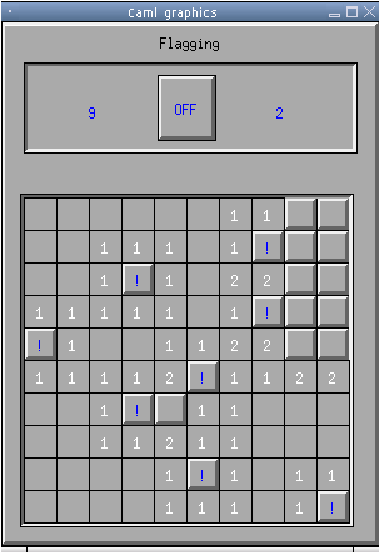
\includegraphics[scale=0.5]{drafts/book012}}
	\caption{\label{fig:screenshot}Снимок экрана}
\end{figure}

Разделим реализацию программы на три части.
\begin{enumerate}
	\item описание абстрактной игры, состоящей из внутреннего представления 
минного поля и функций управляющих этим представлением.

	\item графическое описание игры с соответствующими функциями рисования 
клеток.

	\item часть, отвечающая за взаимодействие между двумя предыдущими частями. 
\end{enumerate}

\subsection{Абстрактное минное поле}
\label{subsec:the_abstract_mine_field}

В этой части мы рассмотрим минное поле как абстрактную сущность, не уделяя 
внимания способам вывода на экран.

\paragraph{Конфигурация}

Минное поле характеризуется своими размерами и числом заминированных клеток. 
Сгруппируем эти три параметра в одной записи и определим конфигурацию по 
умолчанию: размер $10 \times 10$ и $15$ мин.

\begin{lstlisting}[language=OCaml]
# type config = { 
   nbcols  : int ;
   nbrows : int ; 
   nbmines : int };;
# let default_config = { nbcols=10; nbrows=10; nbmines=15 } ;;
\end{lstlisting}

\paragraph{Минное поле}

Вполне естественно будет определить минное поле как двумерный массив. Так же 
нужно уточнить натуру элементов массива и информацию, которую необходимо знать 
для каждого из них. Состояние клетки может быть: 

\begin{itemize}
	\item клетка заминирована?

	\item клетка открыта?

	\item клетка помечена?

	\item сколько из окружающих ячеек заминировано? 
\end{itemize}

Последняя информация не так важна, это значение можно вычислить в нужный момент. 
Но будет проще сделать данный расчёт раз и навсегда в начале игры.

Клетка представлена записью с четырьмя полями, хранящими вышеуказанную 
информацию.

\begin{lstlisting}[language=OCaml]
# type cell = { 
   mutable mined : bool ;
   mutable seen : bool ; 
   mutable flag : bool ; 
   mutable nbm : int
 } ;;
\end{lstlisting}

Двумерный массив есть вектор векторов клеток.

\begin{lstlisting}[language=OCaml]
# type board = cell array array ;;
\end{lstlisting}

\paragraph{Итератор}

Далее в программе нам понадобится применять функцию к каждой клетке поля. 
Реализуем универсальный итератор \code{iter\_cells}, который применяет 
указанную функцию \code{f} к каждому элементу массива конфигурации \code{cf}.

\begin{lstlisting}[language=OCaml]
# let iter_cells cf f = 
   for i=0 to cf.nbcols-1 do for j=0 to cf.nbrows-1 do f (i,j) done done ;;
val iter_cells : config -> (int * int -> 'a) -> unit = <fun>
\end{lstlisting}

Здесь мы получили хорошее сочетание функционального и императивного стилей. Для 
итеративного применения функции с побочным эффектом (она не возвращает 
результат) ко всем элементам массива, используется функция высшего порядка 
(функция, аргумент которой есть другая функция).

\paragraph{Инициализация}

Расположение заминированных клеток будет определяться случайно. Для $r$ и $c$, 
число линий и колонок заминированного поля, и $m$ число мин, необходимо 
получить список состоящий из $m$ чисел в интервале от $1$ до $r * c$. В 
алгоритме подразумевается, что $m < r * c$, однако необходимо сделать эту 
проверку в программе.

Простым решением этой задачи будет создание пустого списка. Затем мы генерируем 
случайное число и размещаем его в список, если оно уже не принадлежит списку. 
Повторим эту операцию до тех пор, пока в списке не будет $m$ чисел. Для этих 
целей, воспользуемся следующими функциями из модулей {\it Random} и {\it Sys}:

\begin{itemize}
	\item \code{Random.int}: \type{int -> int} для входного аргумента $n$ 
возвращает случайное число в диапазоне от $0$ до $n - 1$. 

	\item \code{Random.init}: \type{int -> unit}, инициализация генератора 
случайных чисел.

	\item \code{Sys.time}: \type{unit -> float} возвращает время использования 
процессора в миллисекундах с начала запуска программы. Эта функция используется 
при инициализации генератора случайных чисел при каждой новой игре. 
\end{itemize}

Модули, содержащие эти функции, описаны в главе  \ref{??} на страницах \ref{??} 
и \ref{??} соответственно.

У функции, случайно выбирающей заминированные клетки, два аргумента: общее число 
клеток (\code{cr}) и число мин (\code{m}). Она возвращает список из \code{m} 
линейных координат. 

\begin{lstlisting}[language=OCaml]
# let random_list_mines cr m = 
   let cell_list = ref [] 
   in while (List.length !cell_list) < m do 
        let n = Random.int cr in
         if not (List.mem n !cell_list) then cell_list := n :: !cell_list 
      done ;
     !cell_list ;;
val random_list_mines : int -> int -> int list = <fun>
\end{lstlisting}

Мы не можем заявить что эта функция, так она написана, закончится через 
определённое число итераций. Если генератор случайных чисел достаточно хороший, 
то можно лишь с уверенностью сказать, что вероятность того что эта функция не 
закончится равна нулю. Откуда мы получаем парадоксальное суждение: \enq{функция 
закончится если она выполняется бесконечно}. Однако, на практике эта функция 
никогда нас не подводила, поэтому удовольствуемся данным негарантированным 
определением для генерации списка заминированных клеток.

Для того, чтобы при каждой новой игре получить разные заминированные клетки, 
нужно инициализировать генератор случайных чисел. Инициализировать будем при 
помощи процессорного времени в миллисекундах, которое истекло с момента запуска 
программы.

\begin{lstlisting}[language=OCaml]
# let generate_seed () =
   let t = Sys.time () in
   let n = int_of_float (t*.1000.0) 
   in Random.init(n mod 100000) ;;
val generate_seed : unit -> unit = <fun>
\end{lstlisting}

Практика показывает, что одна и та же программа затрачивает в среднем одинаковое 
время, из–за чего мы получаем схожий результат функции \code{generate\_seed}. В 
связи с этим, функция \code{Unix.time} предпочтительней (см. гл. \ref{??}).

Во время инициализации минного поля, а так же в ходе игры, необходимо знать для 
данной клетки число окружающих заминированных клеток (функция 
\code{neighbors}). При вычислении множества соседних клеток, мы учитываем 
крайние клетки, у которых меньше соседей, чем у тех что находятся в середине 
поля (функция \code{valid}).

\begin{lstlisting}[language=OCaml]
# let valid cf (i,j) = i>=0 && i<cf.nbcols && j>=0 && j<cf.nbrows  ;;
val valid : config -> int * int -> bool = <fun>
# let neighbors cf (x,y) =
   let ngb = [x-1,y-1; x-1,y; x-1,y+1; x,y-1; x,y+1; x+1,y-1; x+1,y; x+1,y+1]
   in List.filter (valid cf) ngb ;;
val neighbors : config -> int * int -> (int * int) list = <fun>
\end{lstlisting}

Инициализация минного поля реализуется функцией \code{initialize\_board}, она 
выполняет четыре задачи:

\begin{enumerate}
	\item генерация списка заминированных клеток

	\item создание двумерного массива состоящего из разных клеток

	\item пометка заминированных клеток

	\item вычисление количества заминированных соседних клеток для каждой 
не заминированной клетки
\end{enumerate}

В этой функции используется несколько локальных функций, которые мы вкратце 
опишем.

\begin{enumerate}
	\item \code{cell\_init}: получить начальные значения клетки.

	\item \code{copy\_cell\_init}: инициализация клетки.

	\item \code{set\_mined}: заминировать клетку.

	\item \code{count\_mined\_adj}: для конкретной клетки вычислить количество 
соседних заминированных клеток.

	\item \code{set\_count}: для конкретной не заминированной клетки обновить 
количество заминированных соседних клеток. 
\end{enumerate}

\begin{lstlisting}[language=OCaml]
# let initialize_board cf = 
   let cell_init () = { mined=false; seen=false; flag=false; nbm=0 } in 
   let copy_cell_init b (i,j) = b.(i).(j) <- cell_init() in
   let set_mined b n = b.(n / cf.nbrows).(n mod cf.nbrows).mined <- true
   in
   let count_mined_adj b (i,j) =
     let x = ref 0 in
     let inc_if_mined (i,j) = if b.(i).(j).mined then incr x 
     in List.iter inc_if_mined (neighbors cf (i,j)) ;
        !x
   in
   let set_count b (i,j) =
     if not b.(i).(j).mined 
     then b.(i).(j).nbm <- count_mined_adj b (i,j)
   in
   let list_mined = random_list_mines (cf.nbcols*cf.nbrows) cf.nbmines in 
   let board = Array.make_matrix cf.nbcols cf.nbrows (cell_init ()) 
   in iter_cells cf (copy_cell_init board) ;
      List.iter (set_mined board) list_mined ;
      iter_cells cf (set_count board) ;
      board ;;
val initialize_board : config -> cell array array = <fun>
\end{lstlisting}

\paragraph{Открытие клетки}

Если во время игры игрок открывает клетку у которой нет ни одного 
заминированного соседа, он с уверенностью может открыть соседние клетки, до тех 
пор пока есть такие клетки. Для того, чтобы избавить игрока от этой нудного 
момента игры, не требующего размышления, игра сама откроет нужные клетки в этом 
случае. При открытии клетки функция \code{cells\_to\_see} возвращает список 
клеток которые можно открыть.

Идея алгоритма достаточно просто излагается: если у открытой клетки есть 
заминированные соседи, то список ограничивается лишь этой самой клеткой, иначе 
список состоит из её соседей, а так же из соседей её соседей. Трудность состоит 
в том, чтобы написать не зацикливающуюся программу, так как клетка является 
соседом самой себе. Надо избежать проверки по несколько раз одной и той же 
клетки поля. Для того, чтобы знать какая клетка была открыта, создадим вектор 
\code{visited} булевых значений. Размер вектора соответствует количеству 
клеток. Если элемент вектора равен \code{true}, это значит что соответствующая 
клетка была исследована. Рекурсивный поиск клеток осуществляется только среди 
не помеченных клеток.

Используя список соседних клеток, функция \code{relevant}, вычисляет два 
под--списка. Каждый под--список состоит из не заминированных, не открытых, не 
помеченных игроком и непроверенных клеток (которым соответствует значение 
\code{false} в векторе \code{visited}, прим. пер.). Первый под--список включает 
соседей, у которых есть как минимум один заминированных сосед, второй состоит 
из соседних клеток без заминированных соседей. Эти клетки помечаются как 
проверенные. Заметим, что помеченные игроком клетки, даже если они на самом 
деле не заминированы, исключаются из списков. Смысл метки заключается как раз в 
том, чтобы избежать открытия клетки.

Функция \code{cells\_to\_see\_rec} рекурсивно реализует цикл поиска. Исходя из 
обновляемого списка клеток, которые необходимо проверить, она возвращает список 
клеток, которые будут открыты. Начальный список содержит лишь последнюю открытую 
клетку, которая помечена как проверенная.

\begin{lstlisting}[language=OCaml]
# let cells_to_see bd cf (i,j) = 
   let visited = Array.make_matrix cf.nbcols cf.nbrows false in 
   let rec relevant = function 
       [] -> ([],[])
     | ((x,y) as c)::t -> 
          let cell=bd.(x).(y)
          in if cell.mined || cell.flag || cell.seen || visited.(x).(y) 
             then relevant t
             else let (l1,l2) = relevant t 
                  in visited.(x).(y) <- true ;
                     if cell.nbm=0 then (l1,c::l2) else (c::l1,l2)
   in 
   let rec cells_to_see_rec = function 
       [] -> []  
     | ((x,y) as c)::t -> 
           if bd.(x).(y).nbm<>0 then c :: (cells_to_see_rec t)
           else let (l1,l2) = relevant (neighbors cf c)
                in  (c :: l1)  @  (cells_to_see_rec (l2 @ t))
   in visited.(i).(j) <- true ;
      cells_to_see_rec [(i,j)]  ;;
val cells_to_see :
  cell array array -> config -> int * int -> (int * int) list = <fun>
\end{lstlisting}

С первого взгляда, аргумент \code{cells\_to\_see\_rec} увеличивается между 
двумя последовательными вызовами функции, тогда как рекуррентное отношение 
основывается на этом аргументе. Соответственно, может возникнуть вопрос --- 
заканчивается ли эта функция? Использование вектора \code{visited} гарантирует, 
что уже проверенная клетка не будет включена в результат \code{relevant}. В то 
же время, клетки, которые добавляются в список проверяемых клеток, происходят 
из \code{relevant}. Этим гарантируется, что определённая клетка будет 
возвращена \code{relevant} всего один раз и в следствии она будет представлена 
в единственном экземпляре в списке проверяемых клеток. Раз количество клеток 
ограничено, значит наша функция тоже закончится.

На этом неграфическая часть игры заканчивается. Рассмотрим стиль 
программирования, которым мы воспользовались. Выбор изменяемых структур данных 
вынуждает использовать императивный стиль с циклами и присвоением. Однако, для 
решения дополнительных задач мы применили списки и функции обработки в 
функциональном стиле. Стиль программирования предписывается структурами данных, 
которыми мы манипулируем. Функция \code{cells\_to\_see} тому хороший пример: 
она использует списки и, вполне естественно, эта функция написана в 
функциональном стиле. Для хранения информации о проверенных клетках мы 
используем вектор, обновление вектора осуществляется императивно. Конечно, мы 
могли бы сделать тоже самое в чисто функциональном стиле, используя список. 
Однако, цена этого решения выше, чем для предыдущего (поиск элемента в списке 
напрямую зависит от размера списка, тогда как для вектора время поиск есть 
константная величина) и оно не является более простым.

\subsection{Игровой интерфейс}
\label{subsec:displaying_the_minesweeper_game}

Эта часть игры зависит от структур данных, которые представляют состояние игры 
(см. \ref{subsec:the_abstract_mine_field}). Цель этой части --- изобразить на 
экране различные компоненты игры, как на рисунке 
\ref{fig:the_main_window_of_minesweeper}. Для этого воспользуемся функциями 
рисования блоков, описанными ранее на 
\ref{subsec:example_drawing_of_boxes_with_relief_patterns}.

\begin{figure}[h]
	\center{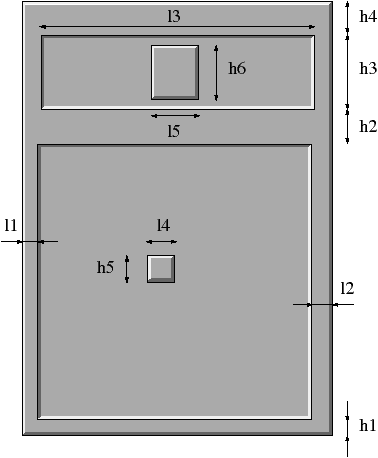
\includegraphics[scale=0.5]{drafts/book013}}
	\caption{\label{fig:the_main_window_of_minesweeper}Основное окно игры}
\end{figure}

Свойства различных компонентов игры описываются следующими параметрами. 

\begin{table}[hl]
\begin{center}
	\label{tbl:operations_on_numbers}
	\caption{Операции над числами}
	\begin{tabular}{|p{7.2cm}|p{7.2cm}|}
	\hline
{\begin{lstlisting}[language=OCaml,frame=none]
# let b0 = 3 ;;
# let w1 = 15 ;;
# let w2 = w1 ;;
# let w4 = 20 + 2*b0 ;;
# let w3 = w4*default_config.nbcols + 2*b0 ;;
# let w5 = 40 + 2*b0 ;;
\end{lstlisting}}
 &
{\begin{lstlisting}[language=OCaml,frame=none]
# let h1 = w1 ;;
# let h2 = 30 ;;
# let h3 = w5+20 + 2*b0 ;;
# let h4 = h2 ;;
# let h5 = 20 + 2*b0 ;;
# let h6 = w5 + 2*b0 ;;
\end{lstlisting}}
\\
	\hline
	\end{tabular}
\end{center}
\end{table}

При помощи этих параметров мы расширим базовую конфигурацию игры (значения с 
типом \code{config}) и определим новую запись \code{window\_config}. В поле 
\code{cf} содержится минимальная конфигурация. Каждой компоненте, изображённой 
на экране, ассоциируем блок: основное окно (поле \code{main\_box}), минное поле 
(поле \code{field\_box}), диалоговое окно (поле \code{dialog\_box}) из двух 
блоков (поля \code{d1\_box} и \code{d2\_box}), кнопка для пометки (поле 
\code{flag\_box}) и текущая клетка (поле \code{current\_box}).

\begin{lstlisting}[language=OCaml]
# type window_config = {
   cf : config ;
   main_box : box_config ;
   field_box : box_config ;
   dialog_box : box_config ;
   d1_box : box_config ;
   d2_box : box_config ;
   flag_box : box_config ;
   mutable current_box : box_config ;
   cell : int*int -> (int*int) ;
   coor : int*int -> (int*int)
 } ;;
\end{lstlisting}

Кроме этого, значение с типом \code{window\_config} содержит две функции:

\begin{itemize}
	\item \code{cell}: для координат данной клетки возвращает координаты её 
блока

	\item \code{coor}: для координат пикселя окна возвращает координаты 
соответствующей клетки.
\end{itemize}

\paragraph{Конфигурация}

Определим функцию, которая создаёт графическую конфигурацию (с типом 
\code{window\_config}) в соответствии с минимальной конфигурацией (с типом 
\code{config}) и вышеописанных параметров. Значения параметров некоторых 
компонент зависят друг от друга. Например, ширина основного блока зависит от 
ширины блока минного поля, которых в свою очередь зависит от количества 
столбцов. Чтобы не вычислять одно и то же по несколько раз, мы будем постепенно 
инициализировать эти поля. В отсутствии специальных функций данный этап 
инициализации немного нудный.

\begin{lstlisting}[language=OCaml]
# let make_box x y w h bw r =
   { x=x; y=y; w=w; h=h; bw=bw; r=r; b1_col=gray1; b2_col=gray3; b_col=gray2 } 
;;
val make_box : int -> int -> int -> int -> int -> relief -> box_config =
  <fun>
# let make_wcf cf = 
   let wcols =  b0 + cf.nbcols*w4 + b0 
   and hrows =  b0 + cf.nbrows*h5 + b0  in
   let main_box =  let gw = (b0 + w1 + wcols + w2 + b0) 
                and gh = (b0 + h1 + hrows + h2 + h3 + h4 + b0)
                in make_box 0 0 gw gh b0 Top
   and field_box = make_box w1 h1 wcols hrows b0 Bot  in
   let dialog_box = make_box  ((main_box.w - w3) / 2)
                              (b0+h1+hrows+h2)
                              w3 h3 b0 Bot
   in 
   let d1_box = make_box (dialog_box.x + b0) (b0 + h1 + hrows + h2)
                         ((w3-w5)/2-(2*b0)) (h3-(2*b0)) 5 Flat  in
   let flag_box = make_box (d1_box.x + d1_box.w) 
                        (d1_box.y + (h3-h6) / 2) w5 h6 b0 Top  in 
   let d2_box = make_box (flag_box.x + flag_box.w) 
                         d1_box.y d1_box.w d1_box.h 5 Flat  in
   let current_box = make_box 0 0 w4 h5 b0 Top
   in { cf = cf; 
        main_box = main_box; field_box=field_box; dialog_box=dialog_box;
        d1_box=d1_box; 
        flag_box=flag_box; d2_box=d2_box; current_box = current_box;
        cell = (fun (i,j) -> ( w1+b0+w4*i , h1+b0+h5*j)) ;
        coor = (fun (x,y) -> ( (x-w1)/w4 , (y-h1)/h5 )) } ;;
val make_wcf : config -> window_config = <fun>
\end{lstlisting}

\paragraph{Вывод клеток}

Теперь нам предстоит определить функции вывода клеток в различных случаях: 
клетка может быть открыта или закрыта, содержать или нет информацию. Вывод 
(блока) текущей клетки всегда будет осуществляться (поле \code{cc\_bcf}).

Определим две функции изменяющие конфигурацию текущей клетки; одна закрывает 
клетку, другая открывает её.

\begin{lstlisting}[language=OCaml]
# let close_ccell wcf i j =
   let x,y = wcf.cell (i,j)
   in wcf.current_box <- {wcf.current_box with x=x; y=y; r=Top} ;;
val close_ccell : window_config -> int -> int -> unit = <fun>
# let open_ccell wcf i j =
   let x,y = wcf.cell (i,j)
   in wcf.current_box <- {wcf.current_box with x=x; y=y; r=Flat} ;;
val open_ccell : window_config -> int -> int -> unit = <fun>
\end{lstlisting}

В зависимости от ситуации, необходимо выводить информацию на клетках. Для 
каждого случая мы определяем функцию.

\begin{itemize}
	\item Вывод закрытой клетки:

\begin{lstlisting}[language=OCaml]
# let draw_closed_cc wcf i j =
  close_ccell wcf i j;
  draw_box wcf.current_box ;;
val draw_closed_cc : window_config -> int -> int -> unit = <fun>
\end{lstlisting}

	\item Вывести открытую клетку с числом мин:

\begin{lstlisting}[language=OCaml]
# let draw_num_cc wcf i j n =
   open_ccell wcf i j ;
   draw_box wcf.current_box ;
   if n<>0 then draw_string_in_box Center (string_of_int n) 
                                   wcf.current_box Graphics.white ;;
val draw_num_cc : window_config -> int -> int -> int -> unit = <fun>
\end{lstlisting}

	\item Вывод клетки, содержащей мину:

\begin{lstlisting}[language=OCaml]
# let draw_mine_cc wcf i j = 
   open_ccell wcf i j ;
   let cc = wcf.current_box 
   in draw_box wcf.current_box ;
      Graphics.set_color Graphics.black ; 
      Graphics.fill_circle (cc.x+cc.w/2) (cc.y+cc.h/2) (cc.h/3) ;;
val draw_mine_cc : window_config -> int -> int -> unit = <fun>
\end{lstlisting}

	\item Вывод заминированной и помеченной клетки:

\begin{lstlisting}[language=OCaml]
# let draw_flag_cc wcf i j =
   close_ccell wcf i j ;
   draw_box wcf.current_box ;
   draw_string_in_box Center "!" wcf.current_box Graphics.blue ;;
val draw_flag_cc : window_config -> int -> int -> unit = <fun>
\end{lstlisting}

	\item Вывод ошибочно помеченной клетки: 

\begin{lstlisting}[language=OCaml]
# let draw_cross_cc wcf i j =
  let x,y = wcf.cell (i,j)
  and w,h = wcf.current_box.w, wcf.current_box.h in
  let a=x+w/4 and b=x+3*w/4 
  and c=y+h/4 and d=y+3*h/4 
  in Graphics.set_color Graphics.red ;
     Graphics.set_line_width 3 ;
     Graphics.moveto a d ; Graphics.lineto b c ;
     Graphics.moveto a c ; Graphics.lineto b d ;
     Graphics.set_line_width 1 ;;
val draw_cross_cc : window_config -> int -> int -> unit = <fun>
\end{lstlisting}

\end{itemize}

В ходе игры, выбор соответствующей функции вывода клетки осуществляется 
следующим:

\begin{lstlisting}[language=OCaml]
# let draw_cell wcf bd i j =
   let cell = bd.(i).(j)
   in match (cell.flag, cell.seen , cell.mined ) with
          (true,_,_)  -> draw_flag_cc wcf i j
        | (_,false,_) -> draw_closed_cc wcf i j
        | (_,_,true)  -> draw_mine_cc wcf i j
        | _           -> draw_num_cc wcf i j cell.nbm  ;;
val draw_cell : window_config -> cell array array -> int -> int -> unit =
  <fun>
\end{lstlisting}

Для вывода клеток в конце игры, воспользуемся специальной функцией. Она немного 
отличается от предыдущих тем, что к концу все клетки должны быть открыты. К тому 
же, на ошибочно помеченных клетках выводится красный крест.

\begin{lstlisting}[language=OCaml]
# let draw_cell_end wcf bd i j =
   let cell = bd.(i).(j)
   in match (cell.flag, cell.mined ) with
          (true,true) -> draw_flag_cc wcf i j
        | (true,false) -> draw_num_cc wcf i j cell.nbm; draw_cross_cc wcf i j
        | (false,true) -> draw_mine_cc wcf i j
        | (false,false) -> draw_num_cc wcf i j cell.nbm ;;
val draw_cell_end : window_config -> cell array array -> int -> int -> unit =
  <fun>
\end{lstlisting}

\paragraph{Вывод остальных компонентов}

Состояние режима отметки клеток отображается выпуклым или вогнутым блоком с 
надписью \code{ON} или \code{OFF}:

\begin{lstlisting}[language=OCaml]
# let draw_flag_switch wcf on =
   if on  then wcf.flag_box.r <- Bot  else wcf.flag_box.r <- Top ;
   draw_box wcf.flag_box ;
   if on  then draw_string_in_box Center "ON" wcf.flag_box Graphics.red
   else draw_string_in_box Center "OFF" wcf.flag_box Graphics.blue ;;
val draw_flag_switch : window_config -> bool -> unit = <fun>
\end{lstlisting}

Выведем надпись о предназначении помечающей кнопки.

\begin{lstlisting}[language=OCaml]
# let draw_flag_title wcf =
   let m = "Flagging" in
   let w,h = Graphics.text_size m in
   let x = (wcf.main_box.w-w)/2
   and y0 = wcf.dialog_box.y+wcf.dialog_box.h in
   let y = y0+(wcf.main_box.h-(y0+h))/2 
   in Graphics.moveto x y ;
      Graphics.draw_string m ;;
val draw_flag_title : window_config -> unit = <fun>
\end{lstlisting}

На протяжении всей игры число клеток, которые осталось открыть и число
помеченных клеток выводится в диалоговом окне с обеих сторон помечающей кнопки.

\begin{lstlisting}[language=OCaml]
# let print_score wcf nbcto nbfc =
   erase_box wcf.d1_box ;
   draw_string_in_box Center (string_of_int nbcto) wcf.d1_box Graphics.blue ;
   erase_box wcf.d2_box ;
   draw_string_in_box Center (string_of_int (wcf.cf.nbmines-nbfc)) wcf.d2_box 
    ( if nbfc>wcf.cf.nbmines then Graphics.red else Graphics.blue ) ;;
val print_score : window_config -> int -> int -> unit = <fun>
\end{lstlisting}

Чтобы нарисовать начальное минное поле, нужно вывести (число линий) $\times$ 
(число столбцов) раз закрытую клетку. Хоть это и один и тот же рисунок каждый 
раз необходимо нарисовать и заполнить прямоугольный и четыре трапеции, на это 
может уйти немало времени. Для ускорения этого процесса, воспользуемся 
следующей техникой: нарисуем один раз клетку, захватим её в виде растрового 
изображения и затем скопируем эту кнопку в нужных местах.

\begin{lstlisting}[language=OCaml]
# let draw_field_initial wcf =
   draw_closed_cc wcf 0 0 ;
   let cc = wcf.current_box  in
   let bitmap = draw_box cc ; Graphics.get_image cc.x cc.y cc.w cc.h  in
   let draw_bitmap (i,j) = let x,y=wcf.cell (i,j)
                           in Graphics.draw_image bitmap x y 
   in iter_cells wcf.cf draw_bitmap  ;;
val draw_field_initial : window_config -> unit = <fun>
\end{lstlisting}

В конце игры, все минное поле открывается и на неправильно помеченных клетках 
ставится красный крест.

\begin{lstlisting}[language=OCaml]
# let draw_field_end wcf bd = 
   iter_cells wcf.cf (fun (i,j) -> draw_cell_end wcf bd i j)  ;;
val draw_field_end : window_config -> cell array array -> unit = <fun>
\end{lstlisting}

И наконец, основная функция вывода на экран открывает графический контекст и 
выводит начальное состояние различных компонент.

\begin{lstlisting}[language=OCaml]
# let open_wcf wcf =
   Graphics.open_graph ( " " ^ (string_of_int wcf.main_box.w) ^ "x" ^
                         (string_of_int wcf.main_box.h)               ) ;
   draw_box wcf.main_box ;
   draw_box wcf.dialog_box ;
   draw_flag_switch wcf false ;
   draw_box wcf.field_box ;
   draw_field_initial wcf ;
   draw_flag_title wcf ;
   print_score wcf ((wcf.cf.nbrows*wcf.cf.nbcols)-wcf.cf.nbmines) 0 ;;
val open_wcf : window_config -> unit = <fun>
\end{lstlisting}

Заметим, что все графические функции используют конфигурацию с типом
\code{window\_config}. Это делает их независимыми от расположения компонент 
игры. Если мы пожелаем изменить это расположение, код функций останется 
неизменным, необходимо будет лишь обновить конфигурацию.

\subsection{Взаимодействие между программой и игроком}
\label{subsec:interaction_with_the_player}

Определим возможные действия игрока:

\begin{itemize}
	\item выбрать, нажатием кнопки, режим пометки или открытия клетки. 

	\item нажать на одну из клеток, для того чтобы ее открыть или пометить. 

	\item нажать на клавишу 'q', для того чтобы покинуть игру. 
\end{itemize}

Напомним, что событие \code{Graphics} должно быть связанно с записью 
(\code{Graphics.status}), в которой хранится информация о текущем состоянии 
клавиатуры и мыши в момент возникновения события. Все события мыши, кроме 
нажатия на кнопку пометки или на клетку минного поля, игнорируются. Чтобы 
различать оба события, создадим соответствующий тип.

\begin{lstlisting}[language=OCaml]
# type clickon = Out | Cell of (int*int) | SelectBox  ;;
\end{lstlisting}

Действия нажатия и отпускания кнопки мыши соответствуют двум разным событиям. 
Если оба события произошли на одной и той же компоненте (клетка минного поля или 
кнопка пометки), то такой клик считается правильным о обрабатывается.

\begin{lstlisting}[language=OCaml]
# let locate_click wcf st1 st2 =
   let clickon_of st = 
     let x = st.Graphics.mouse_x and y = st.Graphics.mouse_y
     in if x>=wcf.flag_box.x && x<=wcf.flag_box.x+wcf.flag_box.w && 
           y>=wcf.flag_box.y && y<=wcf.flag_box.y+wcf.flag_box.h  
        then SelectBox
        else let (x2,y2) = wcf.coor (x,y)
             in if x2>=0 && x2<wcf.cf.nbcols && y2>=0 && y2<wcf.cf.nbrows
                then Cell (x2,y2) else Out
   in 
   let r1=clickon_of st1 and r2=clickon_of st2
   in if r1=r2 then r1 else Out ;;
val locate_click :
  window_config -> Graphics.status -> Graphics.status -> clickon = <fun>
\end{lstlisting}

Сердце программы находится в функции \code{loop} и заключается в ожидании и
обработке событий. Эта функция похожа на \code{skel}, описанной на 
\ref{subsec:program_skeleton}, однако здесь мы точнее определяем тип события 
мыши. Условия остановки цикла следующие:

\begin{itemize}
	\item нажатие на клавишу q (или Q), что рассматривается как желание 
остановить программу.

	\item в случае если игрок открыл заминированную клетку, тогда партия 
проиграна.

	\item в случае если игрок открыл все незаминированные клетки, тогда партия. 
выиграна.
\end{itemize}

Объединим данные, необходимые функциям обрабатывающим взаимодействие с игроком, 
в записи \code{minesw\_cf}.

\begin{lstlisting}[language=OCaml]
# type minesw_cf =
   { wcf : window_config; bd : cell array array;
     mutable nb_flagged_cells : int;
     mutable nb_hidden_cells : int;
     mutable flag_switch_on : bool } ;;
\end{lstlisting}

Эти поля соответствуют:

\begin{itemize}
	\item \code{wcf}: графическая конфигурация.

	\item \code{bd}: матрица клеток.

	\item \code{nb\_flagged\_cells}: булево значение, означающее что игра
находится или нет в режиме пометки.

	\item \code{nb\_hidden\_cells}: число помеченных клеток

	\item \code{flag\_switch\_on}: число незаминированных и неоткрытых клеток 
\end{itemize}

Теперь мы готовы, к тому чтобы написать основной цикл.

\begin{lstlisting}[language=OCaml]
# let loop d f_init f_key f_mouse f_end = 
   f_init ();
   try
     while true do 
       let st = Graphics.wait_next_event 
                  [Graphics.Button_down;Graphics.Key_pressed]  
       in if st.Graphics.keypressed  then f_key st.Graphics.key
          else let st2 = Graphics.wait_next_event [Graphics.Button_up] 
               in f_mouse (locate_click d.wcf st st2)
     done
   with End -> f_end ();;
val loop :
  minesw_cf ->
  (unit -> 'a) -> (char -> 'b) -> (clickon -> 'b) -> (unit -> unit) -> unit =
  <fun>
\end{lstlisting}

Функции инициализации, окончания и обработки клавиатуры достаточно банальны.

\begin{lstlisting}[language=OCaml]
# let d_init d () = open_wcf d.wcf
 let d_end  () = Graphics.close_graph()
 let d_key c = if c='q' || c='Q' then raise End;;
val d_init : minesw_cf -> unit -> unit = <fun>
val d_end : unit -> unit = <fun>
val d_key : char -> unit = <fun>
\end{lstlisting}

Для обработки событий мыши нам понадобится несколько дополнительных функций.


\begin{itemize}
	\item \code{flag\_cell}: реакция на клик на клетку в режиме пометки.

	\item \code{ending}: конец игры. В этом случае открыть все заминированные 
клетки, вывести сообщение о победе или проигрыше и ожидать действия с клавиатуры 
или мыши для того, чтобы закрыть программу.

	\item \code{reveal}: реакция на клик на клетку в режиме открытия (режим 
пометки отключен).
\end{itemize}

\begin{lstlisting}[language=OCaml]
# let flag_cell d i j =
   if d.bd.(i).(j).flag 
   then ( d.nb_flagged_cells <- d.nb_flagged_cells -1; 
          d.bd.(i).(j).flag <- false )
   else ( d.nb_flagged_cells <- d.nb_flagged_cells +1; 
          d.bd.(i).(j).flag <- true );
   draw_cell d.wcf d.bd i j;
   print_score d.wcf d.nb_hidden_cells d.nb_flagged_cells;;
val flag_cell : minesw_cf -> int -> int -> unit = <fun>

# let ending d str = 
   draw_field_end d.wcf d.bd;
   erase_box  d.wcf.flag_box;
   draw_string_in_box Center str d.wcf.flag_box Graphics.black;
   ignore(Graphics.wait_next_event 
            [Graphics.Button_down;Graphics.Key_pressed]);
   raise End;;
val ending : minesw_cf -> string -> 'a = <fun>

# let reveal d i j = 
   let reveal_cell (i,j) = 
     d.bd.(i).(j).seen <- true; 
     draw_cell d.wcf d.bd i j;
     d.nb_hidden_cells <- d.nb_hidden_cells -1 
   in 
     List.iter reveal_cell (cells_to_see d.bd d.wcf.cf (i,j));
     print_score d.wcf d.nb_hidden_cells d.nb_flagged_cells;
     if d.nb_hidden_cells = 0 then ending d "WON";;
val reveal : minesw_cf -> int -> int -> unit = <fun>
\end{lstlisting}

Функция, обрабатывающая события мыши, сопоставляет значение типа \code{clickon}.

\begin{lstlisting}[language=OCaml]
# let d_mouse d click = match click with
     Cell (i,j) ->
       if d.bd.(i).(j).seen then ()
       else if d.flag_switch_on then flag_cell d i j 
       else if d.bd.(i).(j).flag then ()
       else if d.bd.(i).(j).mined then ending d "LOST"
       else reveal d i j
   | SelectBox ->
       d.flag_switch_on <- not d.flag_switch_on;
       draw_flag_switch d.wcf d.flag_switch_on
   | Out -> () ;;
val d_mouse : minesw_cf -> clickon -> unit = <fun>
\end{lstlisting}

При создании конфигурации игры, нам необходимо три параметра: число линий, число 
колонок и число мин.

\begin{lstlisting}[language=OCaml]
# let create_minesw nb_c nb_r nb_m = 
   let nbc = max default_config.nbcols nb_c 
   and nbr = max default_config.nbrows nb_r in 
   let nbm = min (nbc*nbr) (max 1 nb_m) in
   let cf = { nbcols=nbc ; nbrows=nbr ; nbmines=nbm } in 
   generate_seed () ;
   let wcf = make_wcf cf in
   {  wcf = wcf ;
      bd = initialize_board wcf.cf;
      nb_flagged_cells = 0; 
      nb_hidden_cells = cf.nbrows*cf.nbcols-cf.nbmines;
      flag_switch_on = false } ;;
val create_minesw : int -> int -> int -> minesw_cf = <fun>
\end{lstlisting}

Функция, запускающая игру, сначала создаёт конфигурацию игры с помощью трёх 
выше указанных параметров и запускает цикл обработки событий.

\begin{lstlisting}[language=OCaml]
# let go nbc nbr nbm = 
   let d = create_minesw nbc nbr nbm in
   loop d (d_init d) d_key (d_mouse d) (d_end);;
val go : int -> int -> int -> unit = <fun>
\end{lstlisting}

Вызов \code{go 10 10 10} запускает игру, показную на изображении 
\ref{fig:screenshot}.

\paragraph{Что дальше?}

Из данной программы можно сделать самостоятельный исполняемый файл. В главе 
\ref{chpt:compilation_and_portability} объяснено как это сделать. После этого 
можно сделать игру более удобной, передавая размер минного поля в командной 
строке. Передача аргументов рассматривается в главе \ref{??}, где приводится 
пример для данной игры (см. \ref{??}).

Другое интересное расширение --- научить машину саму открывать клетки. Для 
этого необходимо уметь определять следующий правильный ход и играть его первым в 
этом случае. Затем вычислить вероятность присутствия мины для каждой клетки и 
играть клетку, для которой это значение минимально.


\part{Средства разработки}
\section*{Содержимое второй части}

Представленные здесь компоненты окружения являются частью дистрибутива Objective
CAML. Это различные компиляторы, многочисленные библиотеки, средства анализа
программы, средства лексического и синтаксического анализа и интерфейса с языком
C.

Objective CAML является компилируемым языком, с двумя способами генерации кода:

\begin{itemize}
	\item byte-code выполняемый виртуальной машиной

	\item нативный код, выполняемый напрямую процессором
\end{itemize}

Интерактивный цикл Objective CAML использует byte-code для выполнения введённых
фраз. Он является первейшим средством помощи при разработке. Интерактивный цикл
позволяет типизировать, компилировать и быстро проверять определения функций. К
тому же он выдаёт значения входных аргументов и возврата функций.

Другие привычные средства разработки входят в дистрибутив: вычисление
зависимостей между файлами, отладка и профилирование. При помощи
средств отладки программы мы можем пошагово выполнять программы, устанавливать
метки остановки и просмотреть значения переменных. Средство анализа выдаёт число
вызовов функций, время затраченное на вызов функции или на выполнение
определённой части кода. Последние два инструмента доступны только на платформах
Unix.

Богатство языка происходит не только из его ядра, но и из различных
библиотек; множество повторно используемых программ, входящих в дистрибутив
языка. Objective CAML тому пример. Графическая библиотека, включённая в
дистрибутив, уже не раз упоминалась. Далее в книге, мы опишем немало новых
библиотек. Они вносят большое число новых возможностей, однако обратной стороной
медали являются некоторые трудности, в особенности в строгости типов.

Какой бы не была богатой библиотека, всегда необходимо уметь связывается с
другим языком программирования. Дистрибутив языка Objective CAML содержит все
необходимое для интерфейса с языком C. То есть мы можем вызывать функции C в
коде Objective CAML и наоборот. Разница в управлении памятью в Objective CAML и
C может стать препятствием в понимании и использовании этого интерфейса. Эта
разница заключается в том, что в Objective CAML имеется автоматический сборщик
мусора.

И в C и в Objective CAML мы можем динамически выделять память и таким образом
достаточно гибко управлять пространством в соответствии с нуждами программы.
Естественно, это имеет смысл лишь если мы можем затем высвободить память для
других нужд выполнения программы. Автоматический сборщик освобождает
программиста от этой задачи, которая является частым источником ошибок и берет
на себя управление сборкой памяти. Эта особенность является одним из элементов
надёжности языка Objective CAML.

Однако, данный механизм отражается (влияет?) на представление данных. То есть
для того, чтобы правильно связывать код на Objective CAML и C, необходимо чётко
представлять себе принципы управления памятью.

В 6 главе мы рассмотрим базовые элементы системы Objective CAML: виртуальная
машина, компиляторы и библиотеки. Здесь мы так же затронем различные методы
компиляции и сравним переносимость с эффективностью.

В 7 даётся глобальный обзор множества типов, функций и исключений, поставляемых
с дистрибутивом. Однако, она не заменяет официального руководства, в котором
подробно описаны эти библиотеки. Но здесь мы рассматриваются новые возможности
предоставляемые некоторыми модуля библиотек. В частности, можно привести пример
форматированного вывода, системный интерфейс и persistence of values

В 8 представлены различные методы автоматической сборки мусора, а затем описан
принцип, используемый сборщиком Objective CAML.

В 9 мы рассмотрим способы отладки программ Objective CAML. Не смотря на
некоторые недостатки, при помощи этих средств можно легко обнаружить проблемное
место программы.

В 10 описываются некоторые проблемы лексического и синтаксического анализа
языка: библиотека регулярный выражений, средства ocamlex и ocamlyacc,
использование потоков (stream).

Сюжет 11 главы — интерфейс с языком C. На сегодня, язык программирования не
может быть полностью изолированным от других. При помощи данного интерфейса,
программы на Objective CAML могут вызвать функцию на C и передать ей значения
Objective CAML и наоборот. Основное затруднение интерфейса заключается в модели
памяти. По этой причине, желательно прочитать главу 8.

В 12 представлены два приложения: обогащённая графическая библиотека, основанная
на иерархической структуре, как AWT2 JAVA, классическая программа поиска пути в
графе с наименьшей стоимостью с новым графическим интерфейсом и кэш--памятью.
\chapter{Компиляция и переносимость}
\label{chpt:compilation_and_portability}

\section {Введение}

Для того, чтобы текст программы превратился в исполняемый модуль, необходимо
выполнить несколько операций. Эти операции сгруппированы в процессе компиляции.
В ходе этого процесса, строится абстрактное синтаксическое дерево (как для
интерпретатора Basic, \ref{??}), затем оно превращается в последовательность
инструкций для реального процессора или для виртуальной машины. В последнем
случае, для того чтобы выполнить программу, необходим интерпретатор инструкций
виртуальной машины. В каждом случае, результат компиляции должен быть связан с
библиотекой времени выполнения, входящей в дистрибутив. Она может меняться в
зависимости от процессора и операционной системы. В неё входят примитивные
функции (такие как операции над числами, системный интерфейс) и менеджер
памяти.

В Objective CAML существует два компилятора. Первый из них --- это компилятор
для виртуальной машины, в результате которого мы получаем байт--код. Второй
компилятор создаёт программу, состоящую из машинного кода,
выполняемого реальным процессором, как Intel, Motorola, SPARC, HP-PA,
Power-PC или Alpha. Компилятор байт--кода отдаёт предпочтение переносимости
кода, тогда как компилятор в машинный код увеличивает скорость выполнения.
Интерактивный интерпретатор, который мы видели в первой части, использует
байт--код. Каждая введённая фраза компилируется и затем выполняется в окружении
символов, определённых в течении интерактивной сессии.
\section {Этапы компиляции}
\label{sec:steps_of_compilation}

Исполняемый файл получается в результате этапов трансляции и компоновки,
изображённых в \ref{tbl:steps_in_the_production_of_an_executable}

\begin{table}[hc]
	\centering
	\caption{\label{tbl:steps_in_the_production_of_an_executable}Порядок
создания исполняемого файла}
	\begin{tabular}{|l|c|}
	\hline
	 & Исходный текст программы \\
	\hline
	препроцессирование & \\
	\hline
	 & Исходный текст программы \\
	\hline
	компиляция & \\
	\hline
	 & Программа на ассемблере \\
	\hline
	ассемблирование & \\
	\hline
	 & Машинные инструкции \\
	\hline
	компоновка & \\
	\hline
	 & Исполняемый код \\
	\hline
	\end{tabular}
\end{table}

Сначала начинается препроцессирование (макроподстановка), которое подставляет
одни части текста вместо других при помощи системы макросов. Затем исходный код
программы транслируется в команды ассемблера, которые потом конвертируются в
машинные инструкции. Наконец, процесс компоновки (линковки) производит
связывание с элементами операционной системы. Этот процесс включает в себя
добавление библиотеки времени исполнения, которая главным образом состоит из
менеджера памяти.

\subsection {Компиляторы Objective CAML}
\label{subsec:the_objective_caml_compilers}

Детали различных этапов генерации кода компиляторов Objective CAML представлены
таблице \ref{tbl:compilation_stages}. Внутреннее представление кода программы,
сгенерированного компилятором, называется промежуточным языком (ПЯ).

\begin{table}[hc]
	\centering
	\caption{\label{tbl:compilation_stages}Этапы компиляции}
	\begin{tabular}{|l|c|}
	\hline
	 & Последовательность символов \\
	\hline
	лексический анализ & \\
	\hline
	 & Последовательность лексем \\
	\hline
	синтаксический анализ & \\
	\hline
	 & Синтаксическое дерево \\
	\hline
	семантический анализ & \\
	\hline
	 & Аннотированное синтаксическое дерево \\
	\hline
	генерация промежуточного кода & \\
	\hline
	 & Последовательность кода в ПЯ \\
	\hline
	оптимизация промежуточного кода & \\
	\hline
	& Последовательность кода в ПЯ \\
	\hline
	генерация псевдокода & \\
	\hline
	 & Программа на ассемблере\\
	\hline
	\end{tabular}
\end{table}

При помощи лексического анализа из последовательности символов, мы получаем
последовательность лексических элементов (лексем). В основном лексемы
соответствуют целым числам, числам с плавающей запятой, строкам и
идентификаторам. Сообщение \texttt{Illegal character} генерируется на этом
этапе анализа.

Синтаксический анализ создаёт синтаксическое дерево, проверяя при этом
последовательность лексем с точки зрения правил грамматики языка. Сообщение
\texttt{Syntax error} указывает на то, что анализируемая часть кода не
соответствует правилам грамматики.

При семантическом анализе просматривается синтаксическое дерево, здесь нас
интересует другой аспект корректности программы. На этом этапе, в Objective CAML
происходит вывод типа и, если он прошёл удачно, то выводимый тип является самым
общим типом для выражения или объявления. Сообщения об ошибке типа генерируются
на данном этапе. В этот же момент выявляются случаи, в которых тип члена
последовательности отличен от \texttt{unit}. Могут возникать и другие
предупреждения, возникающие на пример во время анализа сопоставления с образцом
(\texttt{pattern matching is not exhaustive}, \texttt{part of pattern matching
will not be used}).

При генерации и оптимизации промежуточного кода не выводится никаких сообщений
об ошибках или предупреждений. Эти этапы манипуляции промежуточными структурами
позволяют факторизовать разработку различных компиляторов Objective CAML.

Генерация исполняемого модуля --- это финальный этап компиляции, который зависит
от компилятора.

\subsection {Описание компилятора байт-кода}

Виртуальная машина Objective CAML называется Zinc (от \enq{Zinc Is Not Caml}).
Она была создана Гзавье Леруа (Xavier Leroy) и описана в (\cite{??}). Это имя
было выбрано, для того чтобы подчеркнуть разницу между первыми реализациями
языка Caml, основанного на виртуальной машине CAM (от Categorical Abstract
Machine, см. \cite{??}).

На рисунке \ref{fig:virtual_machine} изображена виртуальная машина Zinc. В
первой части представлен интерпретатор связанный с библиотекой. Вторая часть
соответствует компилятору, который генерирует байт--код для машины Zinc. Третья
часть содержит библиотеки, идущие вместе с компилятором. Они более подробно
описаны в главе \ref{chpt:libraries}.

\begin{figure}[ch]
	\center{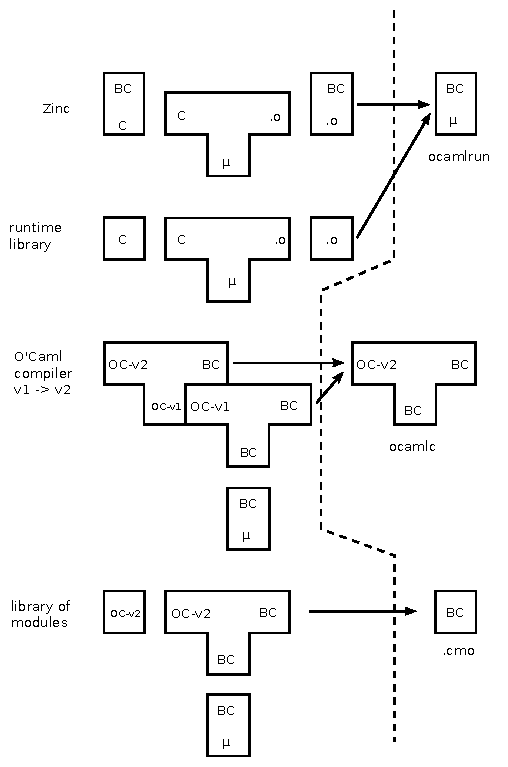
\includegraphics {img/virtual_machine}}
	\caption{\label{fig:virtual_machine}Виртуальная машина}
\end{figure}

Графические символы, используемые на рисунке \ref{fig:virtual_machine}, являются
стандартной нотацией в области компиляторов. Простой блок символизирует файл,
написанный на языке, который указан внутри блока. Двойной блок представляет
интерпретацию одного языка программой, написанной на другом языке. Тройной блок
--- исходный язык компилируется в машинный при помощи компилятора, написанном на
третьем языке. Символы, соответствующие интерпретаторам и компиляторам,
изображены на рисунке
\ref{fig:graphical_notation_for_interpreters_and_compilers}.

\begin{figure}[h]
	\center{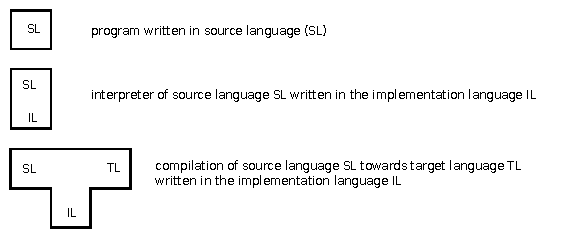
\includegraphics
{img/graphical_notation_for_interpreters_and_compilers}}
	\caption{\label{fig:graphical_notation_for_interpreters_and_compilers}
Символы интерпретаторов и компиляторов}
\end{figure}

Пояснение к рисунку \ref{fig:virtual_machine}:

\begin{itemize}
	\item BC: байт-код машины Zinc

	\item C: код C

	\item .o: объектный файл, зависящий от используемой архитектуры

	\item $\mu$: микропроцессор

	\item OC (v1 или v2): код Objective CAML
\end{itemize}


{\it Замечание}

Основная часть компилятора Objective CAML написана на языке Objective CAML.
Переход с версии v1 на версию v2 изображён на второй части рисунка
\ref{fig:virtual_machine}.

\section{Типы компиляции}
\label{sec:compilation}

Дистрибутив языка зависит от типа процессора и операционной системы. В
дистрибутив Objective CAML для каждой архитектуры (пара: процессор, операционная
система) входит интерактивная среда интерпретатора, байт--код компилятор, и, в
большинстве случаев, компилятор машинного кода для данной архитектуры.

\subsection{Названия команд}
\label{subsec:command_names}

В таблице \ref{tbl:commands_for_compiling} приводятся названия различных
компиляторов, входящих в дистрибутив Objective CAML. Первые четыре из них
являются частью каждого дистрибутива.

\begin{table}
	\begin{tabular}{|l|l|}
	\hline
	\texttt{ocaml} & интерактивная среда интерпретатора \\
	\hline
	\texttt{ocamlrun} & интерпретатор байт--кода \\
	\hline
	\texttt{ocamlc} & компилятор в байт--код \\
	\hline
	\texttt{ocamlopt} & компилятор машинного кода \\
	\hline
	\texttt{ocamlc.opt} & оптимизированный компилятор байт--кода \\
	\hline
	\texttt{ocamlopt.opt} & оптимизированный компилятор машинного кода \\
	\hline
	\texttt{ocamlmktop} & конструктор новых сред интерпретатора \\
	\hline
	\end{tabular}
	\caption{\label{tbl:commands_for_compiling}Команды
компиляции}
\end{table}

Оптимизированные компиляторы были сами скомпилированы компилятором машинного
кода. Они компилируют быстрее, но в остальном идентичны неоптимизированным
версиям.

\subsection{Единица компиляции}

Единица компиляции соответствует наименьшей части программы на Objective CAML,
которая может быть скомпилирована. Для интерактивного интерпретатора таким
элементом является фраза на языке Objective CAML, тогда как для пакетных
компиляторов таким элементом является пара файлов: исходный код и файл
интерфейсов, где файл интерфейсов не обязателен. Если он отсутствует, то все
глобальные объявления файла--исходника будут видны другим элементам компиляции.
Создание интерфейсных файлов будет рассмотрено в главе \ref{??}, посвящённой
модульному программированию. Эти файлы отличаются друг от друга расширением
имени файла.

\subsection{Расширения файлов Objective CAML}

В таблице \ref{tbl:file_extensions} представлены расширения файлов, используемые
для программ Objective CAML и C.

\begin{table}[hc]
	\centering
	\caption{\label{tbl:file_extensions}Расширения файлов}
	\begin{tabular}{|l|l|}
	\hline
	расширение & значение \\
	\hline
	\texttt{.ml} & исходник \\
	\hline
	\texttt{.mli} & интерфейсный файл \\
	\hline
	\texttt{.cmo} & объектный файл (байт--код) \\
	\hline
	\texttt{.cma} & объектный файл библиотеки \\
	\hline
	\texttt{.cmi} & скомпилированный интерфейсный файл \\
	\hline
	\texttt{.cmx} & объектный файл (нативный) \\
	\hline
	\texttt{.cmxa} & объектный файл библиотеки (нативный) \\
	\hline
	\texttt{.c} & исходник на C \\
	\hline
	\texttt{.o} & объектный файл C (нативный) \\
	\hline
	\texttt{.a} & объектный файл библиотеки C (нативный) \\
	\hline
	\end{tabular}
\end{table}

Файлы \texttt{example.ml} и \texttt{example.mli} формируют единицу компиляции.
Скомпилированный интерфейсный файл (\texttt{example.cmi}) может быть использован
нативным и байт--код компилятором. Файлы на \texttt{C} используются для
интерфейса между Objective CAML и библиотеками, написанными на языке \texttt{C}
(\ref{??}).

\subsection{Байт--код компилятор}

Общая форма команды компиляции следующая:

\begin{lstlisting}[language=Bash]
command options file_name
\end{lstlisting}

Objective CAML подчиняется тому же правилу.

\begin{lstlisting}[language=Bash]
ocamlc -c example.ml
\end{lstlisting}

Перед параметрами компилятора ставится символ \texttt{`-'}, как это принято в
системе \texttt{Unix}. Расширения файлов интерпретируются в соответствии с
таблицей \ref{tbl:file_extensions}. В приведённом примере, файл
\texttt{exemple.ml} рассматривается как исходник на Objective CAML, и после его
компиляции будет сгенерированно два файла \texttt{exemple.cmo} и
\texttt{exemple.cmi}. Опция \texttt{`-c'} указывает компилятору, что необходимо
скомпилировать только объектный файл. Без этой опции компилятор \texttt{ocamlc}
создаст исполняемый файл \texttt{a.out}, то есть в данном случае он реализует
компоновку.

В таблице \ref{tbl:principal_options_of_the_bytecode_compiler} описаны основные
опции байт--код компилятора. Остальные опции приведены в таблице
\ref{tbl:other_options_for_the_bytecode_compiler}.

\begin{table}[hc]
	\centering
	\caption{\label{tbl:principal_options_of_the_bytecode_compiler}Основные
опции байт--код компилятора}
	\begin{tabular}{|l|l|}
	\hline
	\texttt{-a} & создать библиотеку \\
	\hline
	\texttt{-c} & компиляция, без редактирования связей \\
	\hline
	\texttt{-o} {\it имя\_файла} & указывает имя исполняемого файла \\
	\hline
	\texttt{-linkall} & связать со всеми используемыми библиотеками \\
	\hline
	\texttt{-i} & вывести все скомпилированные глобальные объявления \\
	\hline
	\texttt{-pp} {\it команда} & использовать {\it команду} как препроцессор \\
	\hline
	\texttt{-unsafe} & отключить проверку индексов \\
	\hline
	\texttt{-v} & вывести версию компилятора \\
	\hline
	\texttt{-w} {\it список} & выбрать, в соответствии со {\it списком}, уровень
предупреждений \\
	\hline
	\texttt{-impl} {\it файл} & указывает, что {\it файл} это исходник на Caml
(см. таб. \ref{tbl:description_of_compilation_warnings}) \\
	\hline
	\texttt{-intf} {\it файл} & указывает, что {\it файл} есть интерфейсный файл
на Caml (.mli) \\
	\hline
	\texttt{-I} {\it каталог} & добавить каталог в список {\it каталогов} \\
	\hline
	\end{tabular}
\end{table}

\begin{table}[hc]
	\centering
	\caption{\label{tbl:other_options_for_the_bytecode_compiler}Другие опции
байт--код компилятора}
	\begin{tabular}{|l|l|}
	\hline
	нити & \texttt{-thread} (см. \ref{??}) \\
	\hline
	отладка & -\texttt{g, -noassert} (см. \ref{??}) \\
	\hline
	автономный исполняемый файл & \texttt{-custom, -cclib, -ccopt, -cc} (см.
\ref{??}) \\
	\hline
	runtime & \texttt{-make-runtime , -use-runtime} \\
	\hline
	C interface & \texttt{-output-obj} (\ref{??}) \\
	\hline
	\end{tabular}
\end{table}

Чтобы получить возможные опции байт--код компилятора, используйте параметр
\texttt{-help}.

В таблице \ref{tbl:description_of_compilation_warnings} описаны различные уровни
предупреждений. Уровень --- это переключатель (включено/выключено), который
символизируется буквой. Заглавная буква включает данный уровень, а прописная
выключает.

\begin{table}[hc]
	\centering
	\caption{\label{tbl:description_of_compilation_warnings}Описание
предупреждений компилятора}
	\begin{tabular}{|l|l|}
	\hline
	Уровни предупреждений & \\
	\hline
	\texttt{A/a} & включить/выключить все сообщения \\
	\hline
	\texttt{F/f} & частичное применение в последовательности \\
	\hline
	\texttt{P/p} & для неполного сопоставления \\
	\hline
	\texttt{U/u} & для лишних случаев в сопоставлении \\
	\hline
	\texttt{X/x} & включить/выключить все остальные сообщения \\
	\hline
	\texttt{M/m} и \texttt{V/v} & for hidden object (см. главу \ref{??}) \\
	\hline
	\end{tabular}
\end{table}

По умолчанию установлен максимальный уровень предупреждений (\texttt{A}).

Пример использования байт--кода компилятора изображён на рисунке
\ref{fig:session_with_bytecode_compiler}.

\begin{figure}[hc]
	\center{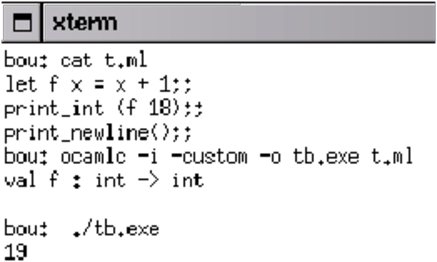
\includegraphics {img/session_with_bytecode_compiler}}
	\caption{\label{fig:session_with_bytecode_compiler}Пример работы с байт--код
компилятором}
\end{figure}

\subsection{Нативный компилятор}

Принцип действия компилятора машинного кода такой же что и байт--код
компилятора, с разницей в сгенерированных файлах. Большинство опций компиляции
те же что проведены в таблицах
\ref{tbl:principal_options_of_the_bytecode_compiler} и
\ref{tbl:other_options_for_the_bytecode_compiler}. Однако, в таблице
\ref{tbl:other_options_for_the_bytecode_compiler} необходимо удалить опции
связанные со средой исполнения. Специфические опции для нативного компилятора
приведены в таблице \ref{tbl:options_specific_to_the_native_compiler}. Уровни
предупреждений остаются теми же.

\begin{table}[hc]
	\centering
	\caption{\label{tbl:options_specific_to_the_native_compiler}Специальные
опции для нативного компилятора}
	\begin{tabular}{|l|l|}
	\hline
	\texttt{-compact} & оптимизация размера кода \\
	\hline
	\texttt{-S} & сохранить код на ассемблере в файле \\
	\hline
	\texttt{-inline} \it{уровень} & установить {\it уровень} \enq{агрессивности}
встраивания функций \\
	\hline
	\end{tabular}
\end{table}

Встраивание является улучшенным методом макроподстановки на стадии
препроцессирования. Оно заменяет вызов функции, подставляя тело функции, в
случае когда аргументы определены. Таким образом несколько вызовов функции
соответствуют новым копиям её тела. Встраиванием мы избавляемся от затрат,
возникающих при инициализации вызова и возврата функции. Однако, расплатой за
это будет увеличение размера кода. Основные уровни встраивания функции
следующие:

\begin{itemize}
	\item $0$: разложение разрешено, в случае если оно не увеличивает размер
кода
	\item $1$: значение по умолчанию, при этом допускается небольшое увеличение
кода
	\item $n > 1$: увеличивает терпимость к увеличению кода
\end{itemize}

\subsection{Интерактивный интерпретатор}

У интерактивного интерпретатора всего две опции:

\begin{itemize}
	\item \texttt{-I} {\it каталог}: добавить каталог в начало списка каталогов,
где находятся
скомпилированные файлы или исходники.
	\item \texttt{-unsafe}: не проверять выход индекса за пределы для векторов и
строк
\end{itemize}

Интерактивный интерпретатор распознает несколько директив, позволяющих
интерактивно изменить его функционирование. Все эти директивы описаны в таблице
\ref{tbl:toplevel_loop_directives}, они начинается с символа \texttt{`\#'} и
заканчиваются привычным \texttt{`;;'}.

\begin{table}[hc]
	\centering
	\caption{\label{tbl:toplevel_loop_directives}Директивы интерпретатора}
	\begin{tabular}{|l|l|}
	\hline
	\texttt{\#quit ;;} & выйти из интерпретатора \\
	\hline
	\texttt{\#directory} {\it каталог} \texttt{;;} & добавить каталог в список
путей \\
	\hline
	\texttt{\#cd каталог} \texttt{;;} & сменить текущий каталог \\
	\hline
	\texttt{\#load} {\it объектный\_файл} \texttt{;;} & загрузить файл .cmo \\
	\hline
	\texttt{\#use} {\it исходный\_файл} \texttt{;;} & скомпилировать и загрузить
исходных файл \\
	\hline
	\texttt{\#print\_depth} {\it глубина} \texttt{;;} & изменить глубину вывода
на экран \\
	\hline
	\texttt{\#print\_length} {\it ширина} \texttt{;;} & аналогично для ширины \\
	\hline
	\texttt{\#install\_printer} {\it функция} \texttt{;;} & указать функцию
вывода на экран \\
	\hline
	\texttt{\#remove\_printer} {\it функция} \texttt{;;} & переключится на
стандартный вывод на экран \\
	\hline
	\texttt{\#trace} {\it функция} \texttt{;;} & трассировка аргументов функции
\\
	\hline
	\texttt{\#untrace} {\it функция} \texttt{;;} & отменить трассировку \\
	\hline
	\texttt{\#untrace\_all ;;} & отменить все трассировки \\
	\hline
	\end{tabular}
\end{table}

Директивы, относящиеся к каталогам, подчиняются правилам используемой
операционной системы.

Директивы загрузки имеют отличное от других директив функционирование. Директива
\texttt{\#use} считывает указанный файл, как если бы он был введён интерактивно.
Директива \texttt{\#load} загружает файл с расширением \texttt{.cmo}. В этом
последнем случае, глобальные декларации этого файла недоступны напрямую. Для
этого необходимо использовать синтаксис с точкой. Если в файле
\texttt{exemple.m} содержится глобальное объявление \texttt{f}, то после
загрузки байт--код ( \texttt{\#load "example.cmo";;}), значение \texttt{f}
доступно как \texttt{Example.f}. Обратите внимание, что первая буква файла ---
заглавная. Этот синтаксис происходит из модульной системы Objective CAML (см.
главу \ref{??}). Директивы настройки глубины и ширины вывода на экран позволяют
контролировать формат выводимых значений, что удобно, когда мы имеем дело с
большими данными.

Директивы трассировки аргументов и результата функции особенно полезны при
отладке программ. Этот вариант использования интерактивного интерпретатора
рассматривается более подробно в главе об анализе программ (\ref{??}).

На рисунке \ref{fig:session_with_the_toplevel_loop} изображён сеанс работы в
интерпретаторе.

\begin{figure}[h]
	\center{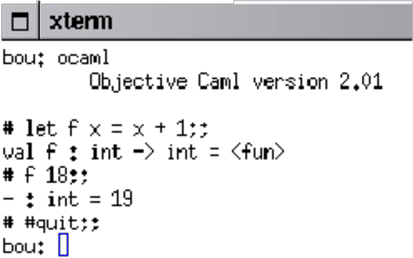
\includegraphics {img/session_with_the_toplevel_loop}}
	\caption{\label{fig:session_with_the_toplevel_loop}Сеанс работы в
интерпретаторе}
\end{figure}

\subsection{Создание интерпретатора}

При помощи команды \texttt{ocamlmktop} мы можем создать новый цикл
интерпретатора, в который загружены определённые библиотеки или модули. Кроме
того, что мы избавляемся от \texttt{\#load} в начале сеанса работы, это так же
необходимо для подключения библиотек на \texttt{C}.

Опции этой команды являются частью опций байт--код компилятора (ocamlc):

\begin{lstlisting}[language=Bash]
-cclib имя\_библиотеки, -ccopt опции, -custom, -I каталог -o имя\_файла
\end{lstlisting}

В главе о графическом интерфейсе (\ref{??}) используется эта команда для
создания цикла содержащего библиотеку \texttt{Graphics} следующим способом:

\begin{lstlisting}[language=Bash]
ocamlmktop -custom -o mytoplevel graphics.cma -cclib \ -I/usr/X11/lib -cclib
-lX11
\end{lstlisting}

Эта команда создаёт исполняемый файл \texttt{mytoplevel}, содержащий байт--код
библиотеки \texttt{graphics.cma}. Этот файл является автономным
(-\texttt{custom}, смотрите следующий раздел) и он связан с библиотекой
\texttt{X11 (libX11.a)}, которая располагается в каталоге \texttt{/usr/X11/lib}.

\chapter{Библиотеки}
\label{chpt:libraries}
\chapter{Автоматический сборщик мусора}

%\section{Введение}
\label{sec:intro_2}

Первый язык функционального программирования LISP появился в конце 1950, в тот
же момент, что и Fortran --- один из первых императивных языков. Оба этих языка
существуют и по сей день, хотя они немало изменились. Область их применения:
вычислительные задачи для Фортрана и символьные (symbolic) для Lisp. Интерес к
функциональному программированию состоит в простоте написания программ, где под
программой подразумевается функция, применённая к аргументам. Она вычисляет
результат, который возвращается как вывод программы. Таким образом можно с
лёгкостью комбинировать программы: вывод одной, становится входным аргументом
для другой.

Функциональное программирование основывается на простой модели вычислений,
состоящей из трёх конструкций: переменные, определение функции и её применение к
какому--либо аргументу. Эта модель, называемая $\lambda$--исчисление, была
введена Alonzo Church в 1932, ещё до появления первых компьютеров. В
$\lambda$--исчислении любая функция является переменной, так что она может быть
использована как входной параметр другой функции, или возвращена как результат
другой. Теория $\lambda$--исчисления утверждает что все то, что вычисляемо может
быть представлено этим формализмом. Однако, синтаксис этой теории слишком
ограничен, чтобы его можно было использовать его как язык программирования. В
связи с этим к $\lambda$--исчислению были добавлены базовые типы (например,
целые числа или строки символов), операторы для этих типов, управляющие
структуры и объявление позволяющие именовать переменные или функции, и в
частности рекурсивные функции.

Существует разные классификации языков функционального программирования. Мы
будем различать их по двум характеристикам, которые нам кажутся наиболее
важными:

\begin{itemize}
	\item без побочных эффектов (чистые), или с побочным эффектом
(не чистые): чистый язык --- это тот, в котором не существует изменения
состояния. Все есть вычисление, и как оно происходит, нас не интересует. Не
чистые языки, такие как Caml или ML, имеют императивные особенности, такие как
изменение состояния. Они позволяют писать программы в стиле близкому к Фортрану,
в котором важен порядок вычисления выражений.

	\item язык типизирован динамически или статически: типизация необходима для
проверки соответствия аргумента, переданного функции, типу формального
параметра. Это проверка может быть выполнена во время выполнения программы. В
этом случае типизация называется динамической. В случае ошибки программа будет
остановлена, как это происходит в Lisp. В случае статической типизации проверка
осуществляется во время компиляции, то есть до выполнения программы. Таким
образом она (проверка) не замедлит программу во время выполнения. Эта типизация
используется в ML и в его диалектах, таких как Objective CAML. Только правильно
типизированные программы, то есть успешно прошедшие проверку типов, могут быть
скомпилированы и затем выполнены.
\end{itemize}

%\section {План главы}

В этой короткой главе представляются средства анализа входящие в дистрибутив
Objective CAML. В первой части описывается команда ocamldep, которая определяет
зависимости множества файлов Objective CAML принадлежащих одной и той же
программе. Во второй части представляются средства отладки, как например
результаты применения функций или стандартное средство отладки — ocamldebug для
операционных систем Unix. В третьей части мы рассмотрим профайлер. Он
анализирует программы и результат этого анализа может быть использован для
оптимизации этой программы.

%\section {Память программы}

Машинные коды программы --- это последовательность инструкций, изменяющих
значения в памяти. Память в основном состоит из следующиъ элементов:

\begin{itemize}
	\item регистры процессора,

	\item стек

	\item сегмент данных (область статического выделения памяти)

	\item куча (область динамического выделения памяти)
\end{itemize}

Только стек ит динамическая область выделения памяти могут менять свой размер
во время работы программы. В зависимости от используемого языка, можно
осуществлять управление данными классами памяти. В то время как программные
инструкции (код) обычно находятся в статической памяти, динамическое связывание
(см. стр. \cite{??}) использует динамическую память.

\chapter{Средства анализа программ}
\label{chpt:program_analysis_tools}

\section {Введение}
\label{sec:intro_10}

Средства анализа программ предоставляют дополнительную информацию, по сравнению
с компилятором или компоновщиком. Часть этих средств реализуют статический
анализ. То есть они анализируют (в виде исходного кода или синтаксического
дерева) и определяют различные свойства кода, такие как зависимости между
модулями или возможные исключения. Другие средства проводят динамический анализ,
то есть изучают программы во время её выполнения. Такие средства полезны, в
случае когда необходимо знать сколько раз была вызвана определённая функция,
какие аргументы были ей переданы или время, затраченное на выполнение части кода
программы. Такие средства анализа могут быть интерактивными, как например
отладчик программ. В этом случае выполнение программы изменяется, для того чтобы
реагировать на команды пользователя, который может установить контрольные точки
чтобы просмотреть значения или перезапустить программу с новыми аргументами.

В дистрибутив Objective CAML входят подобные средства. Некоторые из них имеют не
часто встречающиеся характеристики, связанные со статической типизацией. Такая
типизация гарантирует, что во время выполнения кода, не произойдёт ошибок типа и
используется компилятором для того чтобы генерировать эффективный код небольшого
размера. Часть информации о типе созданных значений теряется и из--за этой
особенности нельзя просмотреть аргументы полиморфных функций.

\section {План главы}
\label{sec:overview_10}

В этой короткой главе представляются средства анализа входящие в дистрибутив
Objective CAML. В первой части описывается команда \code{ocamldep}, которая 
определяет зависимости множества файлов Objective CAML принадлежащих одной и той 
же программе. Во второй части представляются средства отладки, как например
результаты применения функций или стандартное средство отладки --- 
\code{ocamldebug} для операционных систем Unix. В третьей части мы рассмотрим 
профайлер. Он анализирует программы и результат этого анализа может быть 
использован для оптимизации этой программы.

\section {Анализ зависимостей}
\label{sec:dependency_analysis}

Вычисление зависимостей между файлами интерфейса и реализации имеет двойную 
цель. Первая --- получить глобальное видение зависимостей между модулями? 
Вторая --- использовать данную информацию для того чтобы компилировать лишь 
необходимый минимум при изменении некоторых файлов. 

Команда \code{ocamldep} анализирует файлы \code{.ml} и \code{.mli} и выводит 
зависимости файлов в формате Makefile \footnote{Файлы \code{Makefile} 
используются командой \code{make} чтобы обновлять при необходимости файлы или 
программы}.

Зависимости появляются при глобальной декларации других модулей, либо используя 
синтаксис с точкой (пример: \code{M1.f}), либо открывая модуль (пример: 
\code{open M1}).

Предположим, что имеются файлы \code{dp.ml}:

\begin{lstlisting}[language=OCaml]
let print_vect v = 
    for i = 0 to Array.length v do 
      Printf.printf "%f " v.(i)
    done;
    print_newline();;
\end{lstlisting}

и \code{d1.ml}:

\begin{lstlisting}[language=OCaml]
let init n e = 
  let v = Array.create 4 3.14 in 
    Dp.print_vect v;
    v;;
\end{lstlisting}

При вызове команды \code{ocamldep} с указанием файлов, получим следующий 
результат:

\begin{lstlisting}[language=Bash]
$ ocamldep dp.ml d1.ml array.ml array.mli printf.ml printf.mli
dp.cmo: array.cmi printf.cmi 
dp.cmx: array.cmx printf.cmx 
d1.cmo: array.cmi dp.cmo 
d1.cmx: array.cmx dp.cmx 
array.cmo: array.cmi 
array.cmx: array.cmi 
printf.cmo: printf.cmi 
printf.cmx: printf.cmi 
\end{lstlisting}

Зависимости вычисляются для байт--код и нативных компиляторов. Поясним 
полученный результат: компиляция файла \code{dp.cmo} зависит от файлов 
\code{array.cmi} и \code{printf.cmi}. Файлы с расширением \code{.cmi} зависят 
от файлов с таким же именем, но с расширением .mli. Аналогичное правило 
распространяется на файлы \code{.ml} с \code{.cmo} и \code{.cmx}.

Объектные файлы дистирбитува отсутствуют в списке зависимостей. В 
действительности, если команда \code{ocamldep} не найдёт их в текущем каталоге, 
то они будут найдены в каталоге библиотек дистрибутива и выдаст следующий 
результат:

\begin{lstlisting}[language=Bash]
$ ocamldep dp.ml d1.ml
d1.cmo: dp.cmo 
d1.cmx: dp.cmx 
\end{lstlisting}

Для того, чтобы указать командe \code{ocamldep} дополнительные каталоги для 
поиска файлов, используйте опцию \code{-I каталог}.

\section {Профайлер}
\label{sec:profiling}

С помощью профайлера можно получить определённую информацию о выполнении 
программы: сколько раз была выполнения функция или структура контроля 
(условный, цикл или сопоставление с образцом). Эта информация сохраняется в 
файле, анализируя который, можно обнаружить алгоритмические ошибки или 
критические моменты, которые можно оптимизировать.

Для того, чтобы профайлер смог реализовать анализ, необходимо скомпилировать код 
со специальными опциями. Эти опции добавляют в код инструкции, необходимые для 
сбора данных. Существует две методики профайлинга: одна --- для байт--код 
компилятора и другая --- для нативного компилятора, плюс две комманды для 
представления результата. При анализе машинного кода мы получим так же время 
затрачено на выполнение каждой функции.

Профайлинг программы состоит из трёх этапов: 

\begin{itemize}
	\item компиляция с опциями для профайлинга 

	\item выполнение программы

	\item представление результатов
\end{itemize}

\subsection {Команды компиляции}
\label{subsec:compilation_commands}

Ниже приводятся команды компиляции с опциями для профайлинга 

\begin{itemize}
	\item \code{ocamlcp -p} опции для байт--код компилятора

	\item \code{ocamlopt -p} опции для нативного компилятора
\end{itemize}

Указанные компиляторы создают такие же типы файлов, что и обычные команды 
компиляции (\ref{chpt:compilation_and_portability}). В таблице 
\ref{tbl:options_of_the_profiling_commands} приведены различные опции 
компиляции.

\begin{table}[hc]
	\centering
	\caption{\label{tbl:options_of_the_profiling_commands}Опции команд 
профайлинга}
	\begin{tabular}{|l|l|}
	\hline
	\code{f} & вызов функции \\
	\hline
	\code{i} & ответвления {\bf if} \\
	\hline
	\code{l} & цикл {\bf while} и {\bf for} \\
	\hline
	\code{m} & ответвления {\bf match} \\
	\hline
	\code{t} & ответвления {\bf try} \\
	\hline
	\code{a} & все опции \\
	\hline
	\end{tabular}
\end{table}

Данные команды указывают, какие структуры контроля должны учитываться 
профайлером. По умолчанию используются опции \code{fm}.

\subsection {Выполнение программы}
\label{subsec:program_execution}

\subsection {Байт--код компилятор}
\label{subsubsec:bytecode_compiler}

Пру успешном выполнение программы, которая была скомпилирована со 
специальными для профайлера опциями, мы получим файл \code{ocamlprof.dump},
который содержит желаемую информацию.

Вернёмся к нашему примеру произведения элементов целочисленного списка. Пусть 
файл \code{f1.ml} содержит следующий код:

\begin{lstlisting}[language=OCaml]
let rec interval a b = 
  if b < a then []
  else a::(interval (a+1) b);;

exception Found_zero ;; 

let mult_list l = 
 let rec mult_rec l = match l with 
    [] -> 1
  | 0::_ -> raise Found_zero
  | n::x -> n * (mult_rec x)
 in
  try mult_rec l with Found_zero -> 0
;; 
\end{lstlisting}

А так же файл \code{f2.ml}, в котором вызываются функции из \code{f1.ml}:

\begin{lstlisting}[language=OCaml]
let l1 = F1.interval 1 30;;
let l2 = F1.interval 31 60;;
let l3 = l1 @ (0::l2);;

print_int (F1.mult_list l1);;
print_newline();;

print_int (F1.mult_list l3);;
print_newline();;
\end{lstlisting}

Компиляция файлов для профайлера осуществляется так:

\begin{lstlisting}[language=Bash]
ocamlcp -i -p a -c f1.ml
val profile_f1_ : int array
val interval : int -> int -> int list
exception Found_zero
\end{lstlisting}

С опцией \code{-p}, компилятор добавляет новую функцию (\code{profile\_f1\_}) 
для инициализации счётчиков модуля \code{F1}. Это касается и файла \code{f2.ml}:

\begin{lstlisting}[language=Bash]
ocamlcp -i -p a -o f2.exe f1.cmo f2.ml
val profile_f2_ : int array
val l1 : int list
val l2 : int list
val l3 : int list
\end{lstlisting}

\subsection {Нативный компилятор}
\label{subsubsec:native_compiler}

Компиляция в машинный код выглядит следующим образом:

\begin{lstlisting}[language=Bash]
$ ocamlopt -i -p  -c f1.ml
val interval : int -> int -> int list
exception Found_zero
val mult_list : int list -> int
$ ocamlopt -i -p -o f2nat.exe f1.cmx f2.ml
\end{lstlisting}

Здесь используется лишь опция \code{-p} без аргументов. После выполения 
\code{f2.exe} мы получим файл \code{gmon.out}. Формат данного файла распознается 
обычными средствами Unix (см. \code{??}).

\subsection {Представление результата}
\label{subsec:presentation_of_the_results}

Так как способы анализа программ отличаются в зависимости от вида компиляции, 
представление результата соответственно тоже отличается. В случае компиляции в 
байт--код в исходный код программы добавляется число выполнений для структур 
контроля. При компиляции в машинный код для каждой функции добавляется время 
затраченное на её выполнение и число выполнений.

\subsection {Байт--код компилятор}
\label{subsubsec:bytecode_compiler}

Команда \code{ocamlprof} представляет анализ результата измерений профайлера. 
Для этого используется информация содержащаяся в файле \code{camlprof.dump}. 
Данная команда читает приведённый файл и затем, при помощи исходного кода, 
создаёт новый исходный код программы, содержащий желаемые данные в виде 
комментариев.

Для нашего примера получим следующее:

\begin{lstlisting}[language=OCaml]
ocamlprof f1.ml

let rec interval a b = 
  (* 62 *) if b < a then (* 2 *) []
  else (* 60 *) a::(interval (a+1) b);;

exception Found_zero ;; 

let mult_list l = 
 (* 2 *) let rec mult_rec l = (* 62 *) match l with 
    [] -> (* 1 *) 1
  | 0::_ -> (* 1 *) raise Found_zero
  | n::x -> (* 60 *) n * (mult_rec x)
 in
  try mult_rec l with Found_zero -> (* 1 *) 0
;; 
\end{lstlisting}

Полученные счётчики отражают запрошенные в модуле \code{F2} вычисления. Мы 
получили 2 вызова для \code{list\_mult} и 62 для вспомогательной функции 
\code{mult\_rec}. Анализ ответвлений \code{match} показывает что образец по 
умолчанию выполнялся 60 раз, образец [] выполнялся один раз в самом начале и 
образец с нулём в начале списка так же выполнялся один раз, возбуждая 
исключение. В строке с \code{try} указывается значение образца вызвавшее 
исключение.

У команды \code{camlprof} имеется две опции. При помощи опции \code{-f} файл 
можно указать файл, в котором содержатся измерения. Опцией \code{-F} строка 
можно добавить строку в комментарии структурам контроля.

\subsection {Нативный компилятор}
\label{subsubsec:native_compilation}

Чтобы получить время, затраченное на вызов функции умножения элементов списка, 
напишем следующий файл \code{f3.ml}:

\begin{lstlisting}[language=OCaml]
let l1 = F1.interval 1 30;;
let l2 = F1.interval 31 60;;
let l3 = l1 @ (0::l2);;

for i=0 to 100000 do 
  F1.mult_list l1;
  F1.mult_list l3
done;;

print_int (F1.mult_list l1);;
print_newline();;

print_int (F1.mult_list l3);;
print_newline();;
\end{lstlisting}

Это такой же файл как и \code{f3.ml} с 100000 итерациями. 

После выполнения программы получим файл \code{gmon.out}. Формат данного файла 
распознаётся командой \code{gprof}, присутствующей в системе Unix. Вызов этой 
команды выведет на экран затраченное время и граф вызовов. В связи с тем, что 
вывод получается достаточно большой, мы покажем лишь начало, где содержится 
имена функций, которые были вызваны минимум один раз и время затраченное на их 
исполнение.

\begin{lstlisting}[language=Bash]
$ gprof  f3nat.exe 
Flat profile:

Each sample counts as 0.01 seconds.
  %   cumulative   self              self     total
 time   seconds   seconds    calls  us/call  us/call  name
 92.31      0.36     0.36   200004     1.80     1.80  F1_mult_rec_45
  7.69      0.39     0.03   200004     0.15     1.95  F1_mult_list_43
  0.00      0.39     0.00     2690     0.00     0.00  oldify
  0.00      0.39     0.00      302     0.00     0.00  darken
  0.00      0.39     0.00      188     0.00     0.00  gc_message
  0.00      0.39     0.00      174     0.00     0.00  aligned_malloc
  0.00      0.39     0.00      173     0.00     0.00  alloc_shr
  0.00      0.39     0.00      173     0.00     0.00  fl_allocate
  0.00      0.39     0.00       34     0.00     0.00  caml_alloc3
  0.00      0.39     0.00       30     0.00     0.00  caml_call_gc
  0.00      0.39     0.00       30     0.00     0.00  garbage_collection
...
\end{lstlisting}

Здесь наглядно видно, что почти все время выполнения затрачено на исполнение 
функции \code{F1\_mult\_rec\_45}, которая соответствует функции 
\code{F1.mult\_rec} из файла \code{f1.ml}. Мы так же видим, что вызывается 
много других функций. Первые из них, являются функциями стандартной библиотеки 
по управлению памятью(8).




\section{Exercises}
\label{sec:exercises_10}

\section{Резюме}
\label{sec:summary_10}

В данной главе мы ознакомились с различными вспомогательными инструментами 
разработки программ, которые входят в дистрибутив Objective CAML.

Первое из этих средств реализует статический анализ и определяет зависимости 
между множеством элементов компиляции. Эта информация затем интегрируются в файл 
\code{Makefile}, что позволяет компилировать только необходимые файлы. То есть, 
если вы изменили какой--то файл исходник, то необходимо перекомпилировать лишь 
сам файл и зависящие от него файлы, а не всю программы.

Другие средства предоставляют информацию о выполнении программы. Интерактивная 
среда предлагает трассировку выполнения, но, как мы видели, полиморфизм 
устанавливает достаточно серьёзные ограничения на исследуемые значения. Нам 
\enq{видны} лишь мономорфные глобальные объявления, а так же моморфные 
параметры функции. С помощью этого мы все такие можем отслеживать выполнение 
рекурсивных функций. 

И последний инструмент является традиционным в окружении Unix, i.e. отладчик и 
профайлер. При помощи отладчика можно пошагово выполнять программу, а профайлер 
выдаёт информацию о производительности програмы. Оба этих средства могут быть 
использованы в полной мере лишь в среде Unix.

\section{To learn more}
\label{sec:to_learn_more_10}


\chapter{Средства лексического и синтаксического анализа}

\chapter{Взаимодействие с языком C}

\chapter{Приложения}

\section{Введение}
\label{sec:intro_13}

В этой главе представлены два приложения, которые призваны продемонстрировать
пользу от многих подходов к программированию, продемонстрированных ранее.

Первым приложением мы создадим библиотеку графических элементов, \texttt{Awi} 
(Application Window Interface) - Оконный интерфейс приложения. Следующая 
библиотека будет для простого конвертера из франков в Евро. Компоненты 
библиотеки реагируют на ввод со стороны пользователя вызовом обработчиков 
событий. Хотя алгоритмически это простое приложение, оно показывает 
преимущества 
использования замыканий чтобы структурировать взаимодействие между 
компонентами. 
В самом деле, различные обработчики событий имеют общие значения, которые им 
видны через их окружение. Для оценки архитектуры Awi необходимо знать базовую 
графическую библиотеку (\ref{??}).

Второе приложение ищет кратчайший путь в ориентированном графе. Оно использует 
алгоритм Дейкстры, который вычисляет кратчайший путь из исходного узла до всех 
остальных. Механизм кеширования, реализованный через использование таблицы 
слабых указателей (weak pointers) (см. \ref{??}), используется для ускорения 
поиска. Сборщик мусора может удалить элементы таблицы в любое время, но они 
могут быть посчитаны заново при необходимости. Для выбора исходного и 
конечного узла при поиске пути, визуализированный граф использует  простой 
компонент кнопки, взятый из библиотеки \texttt{Awi}. Далее мы сравним 
эффективность работы алгоритма с кешированием и без него. Для облегчения замера 
временных различий между двумя версиями алгоритма, файл с описанием графа и 
источника с конечным узлом подаётся в качестве аргумента поисковому алгоритму. 
В конце небольшой графический интерфейс будет добавлен к программе поиска.



\part{Устройство программы}
\section*{Содержимое третьей части}

\chapter {Модульное программирование}
\chapter{Объектно-ориентированное программирование}

\chapter{Сравнение моделей устройств программ}

\chapter{Приложения}


\part{Параллелизм и распределение}
\chapter{Процессы и связь между процессами}

\chapter{Параллельное программирование}

\chapter{Распределённое программирование}

\chapter{Приложения}

\part{Разработка программ с помощью Objective CAML}


\part{Приложения}

\end {document}
